\documentclass[
			en,
			phd,
			draft,
			garamond,
			12pt,
			]{sty/swathesis}
	

% Intro			 
% Howto			30 (17)
% IDS				40 (27)
% SQLODB		30 (12)
% StackDB		20 (10)
% rel				 5
% Conc			 5


%\newcommand{\tmp}[1]{#1}
\newcommand{\tmpStart}{\color{DarkBlue}}
\newcommand{\tmpEnd}{\color{Black}}
%\newcommand{\tmpStart}{}
%\newcommand{\tmpEnd}{}
\includeonly{introduction}
%\includeonly{introduction, interactive_slicing}
%\includeonly{odb_sql}
%\includeonly{relwork_conclusion}

%\usepackage{parskip}
%% ======================== SETUP =========================
%% Full documentation on all packages can be found at http://google.com or with `texdoc <packagename>`


%% === Tools ==============================================
\usepackage{iftex}
\usepackage{savesym}
%%   - Silence -
%% Disable warnings that don't cause problems
\usepackage{silence}
\WarningFilter{balance}{You have called \balance in second column}
\WarningFilter{caption}{Unsupported document class}
\WarningFilter{caption}{Unused \captionsetup}
\WarningFilter{relsize}{Failed to get list}


%% === Encoding ===========================================
\ifXeTeX
  \usepackage{fontspec}
\else
  \usepackage[utf8]{inputenc}
  \usepackage[T1]{fontenc}
  \input glyphtounicode			%% Copyable unicode in pdf
  \pdfgentounicode=1
\fi


%%% === ACM Template =======================================
%%% Depending on font, may look better with `relayout`
%\usepackage[relayout]{myacm}
%\usepackage{balance}
%%%   - Default font, choose one -
%\usepackage{txfonts}			%% Times Roman, as requested by style guide, creates smaller documents
%%\usepackage[lighttt]{lmodern}	%% Latin Modern, with light typewriter, looks almost like default setting


%% === article Template ===================================
%%   - Font -
\usepackage[lighttt]{lmodern}	%% Latin Modern with light typewriter


%% === Fonts ==============================================
%%   - Other -
%\savesymbol{iint}					%% Better math font
%\savesymbol{iiint}				%
%\savesymbol{iiiint}				%
%\savesymbol{idotsint}			%
\usepackage{MnSymbol}			%% /Better math font
\usepackage[babel=true]{microtype} %% Better kerning


%% === Language ===========================================
\usepackage{babel} 							%% Select language in \documentclass
\usepackage[babel]{csquotes}		%% \enquote, \blockquote
%%   - Quotes -
%% Options for english: british -> '', american -> ""
\ExecuteQuoteOptions{french=guillemets,german=quotes,english=american}
\newcommand\q[1]{\enquote{#1}}	%% Quote with \q{}
\MakeAutoQuote{>}{<} %% {«}{»}
\MakeOuterQuote{"}


%% === Page Format ========================================
%\usepackage{fancyhdr}			%% more header and footer configuration
%\usepackage{pdflscape}			%% \begin{landscape} ... \end{landscape}


%% === Bibliography =======================================
%% use biblatex if you know what you're doing
%\usepackage[
		%%backend=bibtex, 			%% bibtex, no utf-8 support
		%backend=biber,				%% biber backend
		%style=numeric-comp,		%% [1]
		%%style=alphabetic, 		%% [Auth99]
		%%citestyle=authortitle-tcomp,
		%%bibstyle=verbose,
		%%backref=true,
		%defernumbers=true,
		%doi=false,isbn=false,url=false,
		%]{biblatex}
		
		
%% === Images =============================================
\usepackage{graphicx}			%% \includegraphics
\usepackage{subfig}				%% Sub-figures
\DeclareGraphicsExtensions{.pdf,.png,.jpg,.ai}
\DeclareGraphicsRule{.ai}{pdf}{*}{}


%% === Colors =============================================
\usepackage{color}
%\usepackage{colortbl}					%% Colors for tables
\usepackage[svgnames,table]{xcolor}		%% more colors and \rowcolors


%% === Tables =============================================
%\usepackage{ctable}				%% \ctable command
%%  - Table Style -
%% colored rows, requires xcolor
%\newcommand{\insidetable}{\rowcolors*{2}{WhiteSmoke}{white}}
%\setupctable{doinside=\insidetable}


%% === Code Listings ======================================
\usepackage{listings}
%%   - Basic Looks -
\lstset{
	captionpos=b, 
	xleftmargin=0.35cm,
	basicstyle=\smaller\ttfamily, 
	showstringspaces=false, 
	columns=fixed, 
	basewidth={0.5em,0.45em}, 
	upquote=true,
	tabsize=2, 
	gobble=2,
	escapeinside={/*@}{@*/},
	numberbychapter=false,
}
%%   - Linebreaks -
\lstset{
	breaklines=true, 
	breakatwhitespace=true,
	%prebreak=\raisebox{0ex}[0ex][0ex]{\emptyaccsupp{\small\ensuremath{\rhookswarrow}}},
	postbreak=\raisebox{0ex}[0ex][0ex]{\emptyaccsupp{\small\ensuremath{\rcurvearrowse\space}}},
}
%%   - Line Numbers -
\lstset{
	numbers=left, 
	numberstyle=\tiny\emptyaccsupp, 
	numbersep=5pt,
	numberfirstline=true, 
	firstnumber=auto, 
	stepnumber=5,
}
%%   - Copy&Paste -
\lstset{keepspaces=true}
\ifXeTeX
\else
  \makeatletter
  \def\lst@outputspace{{\ifx\lst@bkgcolor\empty\color{white}\else\lst@bkgcolor\fi\lst@visiblespace}}
  \makeatother
	\pdfglyphtounicode{visiblespace}{A0}
	\pdfglyphtounicode{blank}{A0}
	\pdfglyphtounicode{visualspace}{A0}
	\pdfglyphtounicode{uni2423}{A0}
\fi
%%   - Languages -
\lstdefinelanguage{JavaScript}{
	keywords={break, case, catch, continue, debugger, default, delete, do, else, finally, for, function, if, in, instanceof, new, return, switch, this, throw, try, typeof, var, void, while, with},
	morecomment=[l]{//},
	morecomment=[s]{/*}{*/},
	morestring=[b]',
	morestring=[b]",
	sensitive=true,
}
\lstdefinelanguage{HanaSQL}[]{SQL}{
	morekeywords={replace,string,if,daysbetween,secondsbetween,weekday,adddays,addseconds,double},
}
\lstdefinelanguage{algorithm}{
	keywords={break, case, catch, continue, dec, default, delete, do, each, else, end, error, exists, finally, for, function, if, inc, is, new, return, switch, then, this, throw, try, typeof, until, var, void, while, with},
	morestring=[b]",
	morecomment=[l]{//},
	morecomment=[s]{/*}{*/},
	moredelim=[is][\slshape]{'}{'},
	moredelim=[is][\bfseries]{''}{''},
	style=algorithmStyle,
}
\lstdefinestyle{algorithmStyle}{
  literate= % replace with math symbols
			{:=}{{\(\gets\)}}2 {~}{{\(\:\!\!\neg\)}}1
			{<=}{{\(\leq\)}}1 {>=}{{\(\geq\)}}1 
			{!=}{{\(\neq\)}}1 {=}{{\(=\)}}1
			{&&}{{\(\wedge\)}}1 {||}{{\(\vee\)}}1 
			{\{\}}{{\(\emptyset\)}}1
			{\\in}{{\(\in\)}}1
			{\\notin}{{\(\notin\)}}1
			{\\exists}{{\(\exists\)}}1
			{\\nsubseteq}{{\(\subseteq\)}}1
			{<<}{{\(\ll\)}}2
			% escape with \
			{\\:=}{{:=}}2 {\\~}{{\textasciitilde}}1
			{\\<=}{{<=}}2 {\\>=}{{>=}}2 
			{\\!=}{{!=}}2  {\\=}{{=}}1
			{\\&&}{{\&\&}}2 {\\||}{{||}}2 
			{\\\{\}}{{\{\}}}2
			{\\bs}{{\textbackslash}}1 
			{\\'}{{'}}1 
}
%%   - Styles -
\lstdefinestyle{EclipseStyle}{
	keywordstyle=\bfseries\color{Purple},
	stringstyle=\color{Blue},
	commentstyle=\color{Grey},
}
\lstdefinestyle{BWStyle}{
	keywordstyle=\bfseries,
	stringstyle=\color{DimGray},
	commentstyle=\slshape,
}
\lstset{style=BWStyle,language=Java}
\lstMakeShortInline[basicstyle=\ttfamily,language={}]´


%% === More Tools =========================================
%% no changes here
\usepackage{xspace} 			%% \xspace, automatic spaces for custom macros
\usepackage{float}				%% custom floats
\usepackage{mparhack}			%% marginpar hack
% \usepackage{fixltx2e}			%% latex bugs
\usepackage{relsize}			%% \smaller
\usepackage[space=true]{accsupp}
\newcommand\emptyaccsupp[1]{\BeginAccSupp{ActualText={}}#1\EndAccSupp{}}


%% === Misc ===============================================
\usepackage[printonlyused]{acronym}	%% Acronyms
\renewcommand*{\acsfont}[1]{\textsc{#1}}
%% pdfcomments, load before hyperref
\usepackage{pdfcomment}
%% Exclude footnote links from copy&paste
\renewcommand{\thefootnote}{\protect\BeginAccSupp{ActualText={}}\arabic{footnote}\protect\EndAccSupp{}}


%% === Links and Captions =================================
%\usepackage{hyperref}
%\hypersetup{
%%	draft,						%% disable all
	%%% better set this as document option
	%%colorlinks, 				%% color links, instead of bordered
	%hidelinks,					%% for print version
%%% - link colors -
	%linkcolor=Navy,				%% internal, default red
	%citecolor=Navy,				%% citations, default green
	%urlcolor=Purple,			%% URLs, default cyan
	%filecolor=Purple,			%% files, default magenta
%%
	%plainpages=false,
%}

\usepackage[nameinlink, noabbrev]{cleveref}	%% \cref commands
\newcommand{\lineref}[2]{\hyperref[#1]{line~\ref*{#1:#2}}}
\newcommand{\linerefn}[2]{\hyperref[#1]{line~#2}}
\newcommand{\Lineref}[2]{\hyperref[#1]{Line~\ref*{#1:#2}}}
\newcommand{\Linerefn}[2]{\hyperref[#1]{Line~#2}}

%\usepackage[all]{hypcap}
%\usepackage{caption}
%\captionsetup[table]{position=t}
%\captionsetup[subtable]{position=t}


%% === Misc 2 ============================================
\usepackage[xspace]{ellipsis}	%% \dots, load after hyperref


%% === Pdf Options =======================================
\hypersetup{
	draft
	%bookmarksopen,
	%bookmarksnumbered,
%%	pdfstartview={Fit},					%% Fit page
%%	pdfstartview={FitH},				%% Fit width
	%pdfstartview={XYZ null null 1.0},	%% 100% zoom
}

\newcommand{\defaultbaselinestretch}{1.3}
\renewcommand{\baselinestretch}{\defaultbaselinestretch}

\iftrue
\addbibresource{references.bib}
\else
\bibliography{references}
\fi

\setcounter{tocdepth}{1}
\setcounter{secnumdepth}{3}

\renewcommand*{\glsnamefont}[1]{\textbf{#1}}


\usepackage{titlepage}
\TitlePageStyle[discipline=phd, whom={der}, subject=degree]{hpi-swa}
%\degree{Doktor der Naturwissenschaften\\ (Doctor rerum naturalium)}
\degree{Doktor der Ingenieurwissenschaften\\ (Doktor-Ingenieur)}
\faculty{%
Digital Engineering Fakultät\\
der Universität Potsdam}

\advisor{Prof.\,Dr.\,Hasso Plattner}


% ABGABEDATUM
% \setdate{2012}{04}{05}
% \date{\datedate}

\author{Arian Treffer}
\location{Berlin}
\extratitle{\raggedleft Treffer, \\ Omnidb\par}
\title{Omniscient Debugging in Enterprise Applications}
%\subtitle{This is Optionally}
\othertitle{Omniscient Debugging in Unternehmensanwendungen}
%\othersubtitle{Ein Untertitel ist Optional}


%% remove in final version
%\usepackage[colorinlistoftodos]{todonotes}
%\renewcommand{\todo}[2][\empty]{\pdfmargincomment[color=orange,icon=Note,subject=TODO,#1]{#2}}
%\usepackage{pdfcomment}
%\newcommand{\todo}[2][]{\pdfmargincomment[color=orange,icon=Note,subject={TODO},author={#1}]{#2}}


\newacronym{afl}{AFL}{automatic fault-localization}
\newacronym{pdg}{PDG}{program dependence graph}
\newacronym{ddg}{DDG}{dynamic dependence graph}
\newacronym{odb}{ODB}{omniscient debugger}
\newacronym{orm}{ORM}{object-relational mapper}
\newacronym{erp}{ERP}{enterprise resource planning}
%\DeclareAcronym{afl}{short=AFL,long=automated fault-localization}
%\DeclareAcronym{pdg}{short=PDG,long=program dependence graph}
%\DeclareAcronym{ddg}{short=DDG,long=dynamic dependence graph}
%\acrodef{afl}{automated fault-localization}
%\acrodef{pdg}{program dependence graph}
%\acrodef{ddg}{dynamic dependence graph}

\nocite{*}
\begin{document}

\frontmatter
\begin{otherlanguage}{german}
\maketitle
\end{otherlanguage}

\linenumbers

\begin{abstract}
Developers spend between 40 and 60 percent of their time working on defects\todo{ref}.
A lot of that time is spend in the debugger, searching for the cause of an observed problem.
While debugging, a developer's attention is divided between multiple tasks, which fall into two categories:
first, understanding the program at different levels of abstraction and second, operating the debugger and other related tools.
Attention spent in the first category will directly let developers progress towards their goal, whereas the second category represents an overhead that should be kept to a minimum.

Complex enterprise applications often consist of multiple components, such as client code, application layer, and database scripts.
These components are often developed in different programming languages, run in different environments, and therefore require different tools to be debugged.
When debugging such systems, developers can be faced with long infection chains, the paths of erroneous states leading from the fault in the code to the observed failure, that may even cross sub-system boundaries.
%Following an infection chain can be a tedious and time-consuming task,
Back-in-time debuggers can simplify the process of following an infection chain,
 but when execution crosses a system boundary developers have to switch tools and manually map state, such as request arguments, from one system to the next.
This creates an additional mental burden and distracts from the actual problem.

In our work, we take necessary steps towards a debugger that allows developers to efficiently debug long infection chains in a heterogeneous system.

We combine omniscient debugging with dynamic analysis, in particular dynamic slicing, 
to improve the process of tracking erroneous state over long distances.
A new configurable dynamic slicing algorithm processes the debugger's runtime data.
The results are shown in the Slice Navigator, a novel UI component enriching the debugging
experience in multiple ways. Firstly, it supports developers’ short term memory
by providing a summary of relevant program state and context for the current
instruction. Secondly, it provides an alternative to breakpoints as it can be used
to control the debugger to jump to related instructions, such as the last change of
a variable. Thirdly, it allows to directly reconfigure the slicing criteria, enabling
developers to minimize the search space of active code without interrupting the
debugging workflow.

Enterprise applications use a relational database to handle complex operations on large amounts of data.
While most modern databases allow to attach a debugger to queries or scripts, the general tool support for understanding complex programs in databases is rather poor compared to that of popular object-oriented languages.

To accommodate the demand for better debugging tools in database programs, we brought omniscient debugging down to the database.
We developed a method to leverage the mix of imperative control flow and declarative SQL statements in stored procedures. 
This allowed us to created an omniscient debugger which is much more efficient with large amounts of data than previous solutions for object-oriented languages\todo{evaluation results}.

With omniscient debugging available in every component of an enterprise system, we combine the runtime data of each component into an omniscient system debugger that allows to efficiently debug the entire application stack.

\end{abstract}

%\begin{acronym}[XXX]
%\acro{afl}[AFL]{automated fault-localization}
%
%\acro{ddg}[DDG]{dynamic dependence graph}
%\end{acronym}

%\begin{zusammenfassung}
  %zusammenfassung
%\end{zusammenfassung}
\tableofcontents
%\listoffigures
%\listoftables
%\lstlistoflistings
%\printacronyms
%\printglossary[type=main]

\mainmatter
\lstMakeShortInline[basicstyle=\ttfamily,language={Inline}]´

\chapter{Introduction}
\label{sec:introduction}

Twenty years ago, Lieberman 
%described debugging as "the dirty little secret of computer science".
%He 
argued that the huge economic cost created by software bugs, resulting from the efforts to locate and fix bugs and the damages caused by bugs  not found in time, was not adequately matched by efforts to provide better debugging tools and establish better debugging practices.
Lieberman called this the "Debugging Scandal"~\cite{lieberman97:the_debugging_scandal}.
In his famous article, he urged the computer science community to stop ignoring this problem and outlines several directions in which debugging can be evolved.
Twenty years later, computer science research has produced many new and advanced approaches to debugging; in practice, however, the situation has barely improved~\cite{yin11:debugging_scandal_the_next, perscheid17:studying_the_advancement}.

\section{The Real Cost of Software Errors}

The amount of software that is involved in almost every aspect of our modern life is steadily increasing.
In many fields, including traditional engineering fields such as automotive engineering, innovation is largely driven by software these days~\cite{evans08:invisible_engines_how_software, gorschek10:a_lightweight_innovation_process}.
With the rise of cloud computing and devices becoming smarter and smarter, this trend will not stop in the near future, and society vulnerable to software errors.

%Software faults affect the operation of all professional and commercial software products and have been studied in many kinds of applications, such as web-browser~\cite{li06:have_things_changed_now}, enterprise applications~\cite{turhan09:data_mining_source_code, sahoo10:an_empirical_study}, and operating systems~\cite{guo10:characterizing_and_predicting_which}. % check sources
% In Mozilla's Firefox browser, 85\% of bugs were caused by incorrect implementations of requirements~\cite{li06:have_things_changed_now}.

It has long been recognized that there is no such thing as a bug-free program~\cite{schwartz71:an_overview_of_bugs}.
Software faults affect the operation of all professional and commercial software products.
%from web-browsers, over servers, to operating systems~\cite{li06:have_things_changed_now, sahoo10:an_empirical_study, guo10:characterizing_and_predicting_which}.
In 2002, the yearly economic cost of software errors was estimated to be above 60~billion dollars in the United States alone~\cite{tassey02:the_economic_impacts}. 
In 2018, a study estimated the global impact of developer inefficiency, caused by maintenance tasks and debugging, at around 300~billion dollars~\cite{stripe18:the_developer_coefficient}.

These damages are accumulated from a variety of sources.
Most obviously, errors need to be fixed and therefore increase the software development costs.
However, before developers can even begin to work on a fix, the errors have to be reproduced, classified, and prioritized; all activities that cost time and resources~\cite{sahoo10:an_empirical_study, guo10:characterizing_and_predicting_which}.

Further damages are incurred when the increased workload delays the project's release, as the increased time to market can lead to lost opportunities.
Usually, errors are most expensive when they manifest in production.
Not only can they cause direct costs by interrupting business operations, they are also more expensive to repair and can cause long-term damage through loss of reputation and future business for the company.
Additional billions of damage are created by failing software projects, where bugs are often part of the problem~\cite{charette05:why_software_fails}.

%Finally, it is not only the economic damage that is worrisome.
%When software failures occur in critical infrastructure, lives are endangered.
%While total numbers are difficult to determine, there are many reports of incidents where faulty software systems were at least partially responsible for loss of human life~\cite{zhivich09:the_real_cost}.
%\todo{section divider}

\bigskip\noindent
The majority of bugs in modern software systems are semantic bugs, \ie bugs where the code does not implement the intended behavior~\cite{li06:have_things_changed_now}.
Compared to memory or concurrency bugs, semantic bugs are notoriously hard to formalize and detect automatically.

%  between 25\% and
Accordingly, studies found that developers spend up to 60\% of their time on software bugs, debugging, and maintenance related activities~\cite{ballou08:improving_software_quality, hailpern02:software_debugging_testing, beizer03:software_testing_techniques}.
However, effective debugging skills are not only important to reduce development time.
An incorrect bug fix might not cover all corner cases or cause unexpected side-effects, thereby causing additional problems in the future.
In the Apache bug database, 9\% of bug reports were reopened due to bad fixes~\cite{gu10:has_the_bug_really}.
This number does not even include bad fixes for which a new bug report was created.
In a commercial operating system, between 15\% and 24\% of fixes for post-release bugs found were found incorrect and caused additional problems to users; for concurrency bugs, 39\% of fixes were faulty~\cite{yin11:how_do_fixes_become}.

\bigskip\noindent

Interviews across six developed countries found that C-level executives consider access to developers a bigger threat to business success than access to capital~\cite{stripe18:the_developer_coefficient}.
Considering the total cost and development time wasted by bugs in software, we would expect companies to encourage software developers to improve their debugging skills (e.g., through trainings) and to use modern debugging techniques~\cite{zhivich09:the_real_cost}.
However, 72\% of software companies report their debugging practices to be problematic~\cite{ballou08:improving_software_quality}.
Not only do many debuggers lack a formal education in general debugging best practices, there is also a big gap between the state of the art in research and practice.


%\cite{beck_03_testdriven_development_by_example, williams_03_testdriven_development_as}

\section{35 Years of Debugging Research are Barely Used in Practice}

Ever since Grace Hopper famously taped into a log book a moth that was causing computer errors~\cite{hopper47:log_book_with_computer}, thereby bringing the term "debugging" into software engineering, a lot of work has been done to help developers to locate bugs in their software.
\Cref{fig:debugging-timeline} shows a few milestones in the development of debugging techniques.


\begin{figure*}[t]
\centering
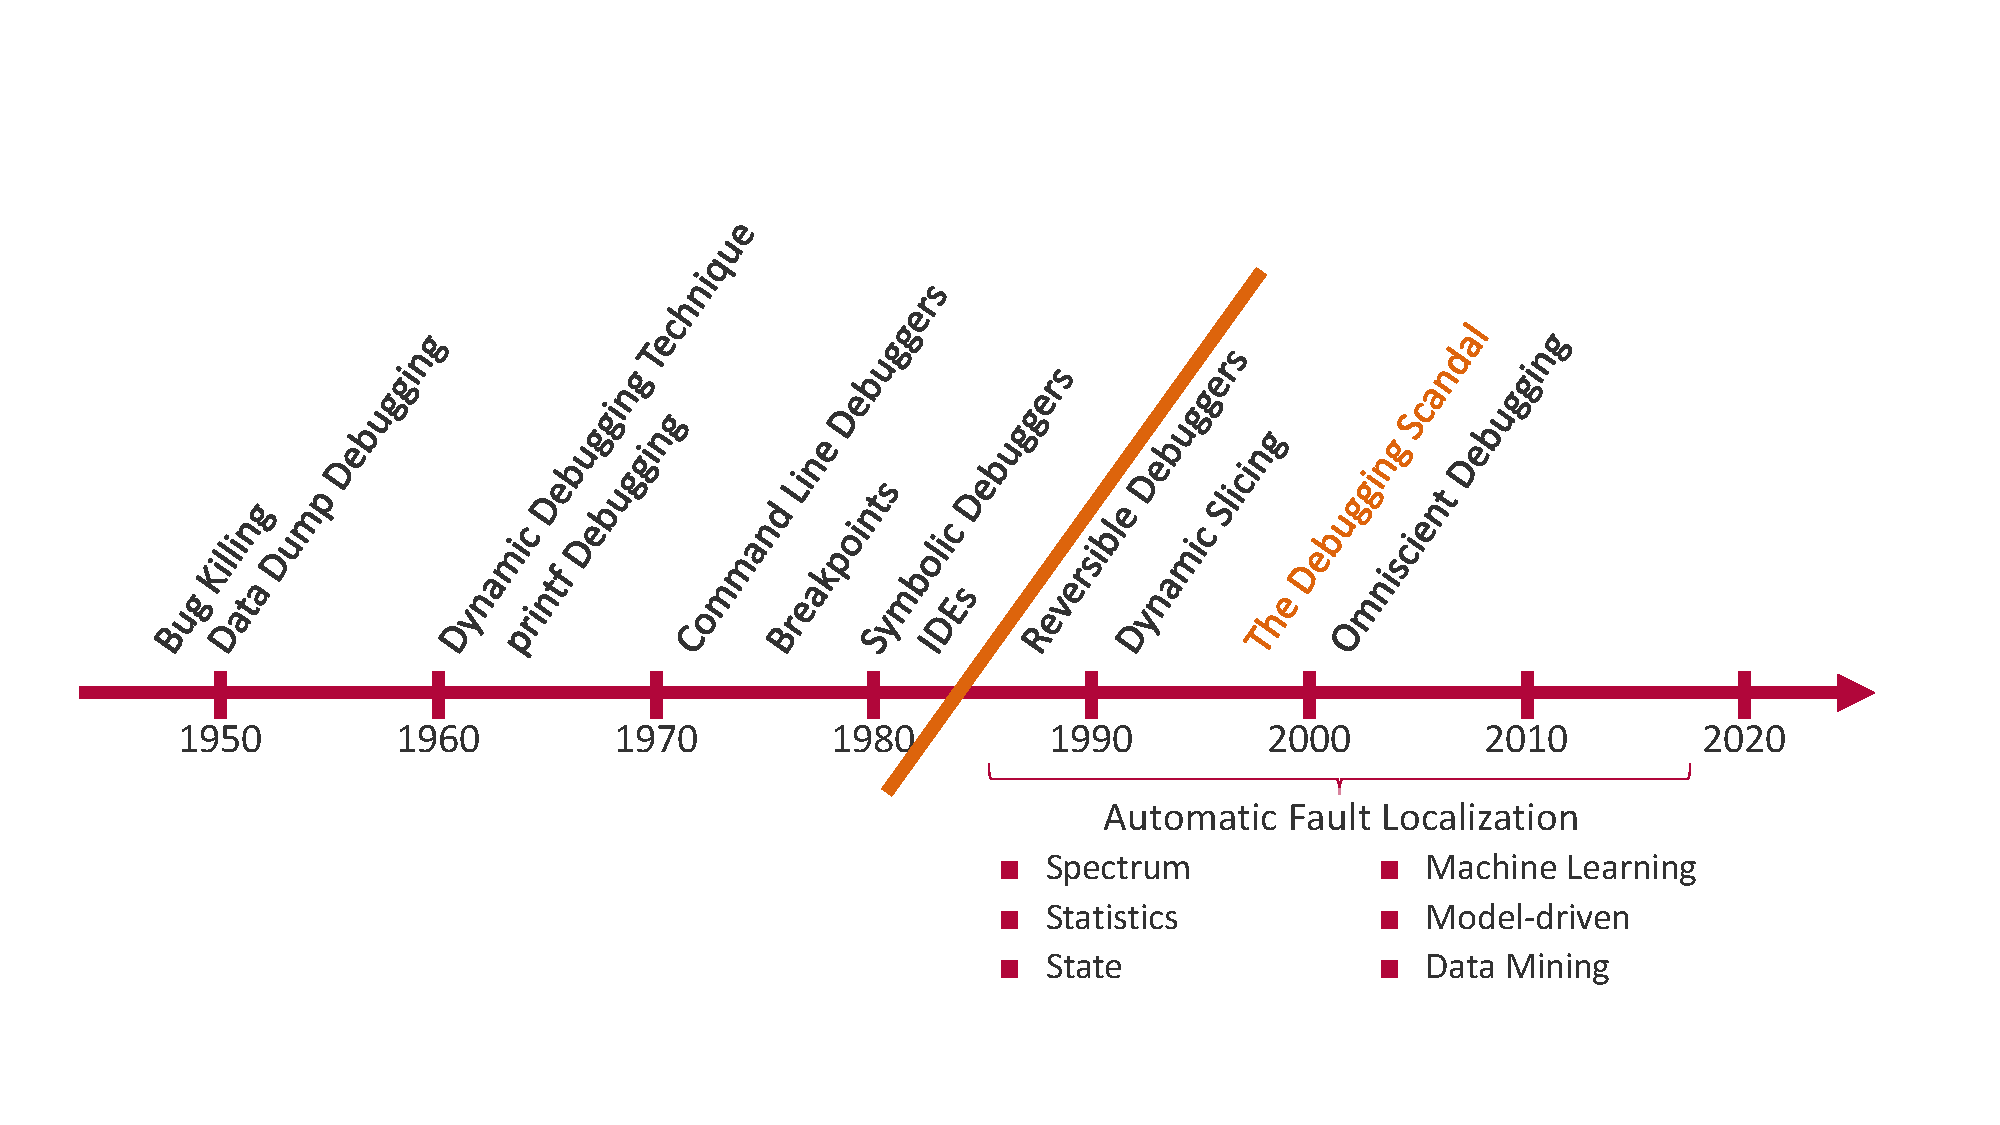
\includegraphics[width=\linewidth]{img/debugging-timeline}
\caption[A brief timeline of debugging history]{A brief timeline of debugging history. The orange line visualizes the gap between research and practice.}
\label{fig:debugging-timeline}
\end{figure*}

Back in the 1940s and 50s, debugging had to be done statically.
In the best case, a post-mortem data dump from the moment of the failure was available.
Because modifying and re-running a program was expensive and time-consuming, bugs could only be located by manually analyzing the code.

%\newpage
In the 1960s, the invention of operating systems with time-sharing capabilities allowed developers to use the "edit -- compile -- run" loop~\cite{linton90:the_evolution_of_dbx}.
By experimenting with changes to the source code, it was much easier to get an understanding of the problem.
Furthermore, interactive terminals allowed developers to insert trace statements into the code, which could report internal states and program flow.
This practice is also known as "printf"-debugging and, although generally considered a bad practice~\cite{zeller09:why_programs_fail}, remains popular to this day~\cite{perscheid17:studying_the_advancement}.

At the same time, with the "Dynamic Debugging Technique" (DDT) and later EXDAMS, the first tools were developed to facilitate stepwise executions of programs and to let developers examine program state~\cite{balzer69:exdams_extendable_debugging}\todo{source: ddt}.
In the 1970s, debuggers moved to the command line and the introduction of the breakpoint allowed developers to pause the execution at predefined points.
In 1975, the first debugger (for COBOL) integrated compiler information to translate identifiers from the source code into memory addresses and vice versa, alleviating developers from manually performing this task.
Such symbolic debuggers are widely used today, unfortunately, as we will see, they are also the most recent innovation that found wide adoption in pracitce~\cite{perscheid17:studying_the_advancement}.

In 1981, Weiser introduced the concept of slices, subsets of statements in a program that influence each other~\cite{weiser81:program_slicing}. 
He showed that slices are a useful abstraction for programmers who think about code~\cite{weiser82:programmers_use_slices_when}.
Later this concept was extended to consider runtime data for higher precision~\cite{agrawal90:dynamic_program_slicing, korel90:dynamic_slicing_of_computer}.

Early on it was noted that given the way developers follow infection chains, by trying to find the source for an incorrect value, it would be helpful to go backwards through a program execution.
Debuggers that used snapshots~\cite{feldman88:igor_a_system} or reverse execution~\cite{lieberman95:zstep_95_a_reversible} were developed in the 1990s.
In 2003, Lewis introduced the concept of "omniscient debugging".
An \ac{odb} can not only run forwards and backwards in time, but has constant-time access to every program state in past, present, and future~\cite{lewis03:debugging_backwards_in_time}.

Although both slicing and omniscient debugging can answer many \linebreak questions developers have while debugging that regular debuggers can't \linebreak answer~\cite{ko07:information_needs_in_collocated, storey97:how_do_program_understanding, sillito06:questions_programmers_ask}, neither technique is widely used, or even widely known, today~\cite{perscheid17:studying_the_advancement}.
As \cref{fig:tool-usage} shows, the same is true for many other modern debugging and \ac{afl} techniques.

\begin{figure*}[t]
\centering
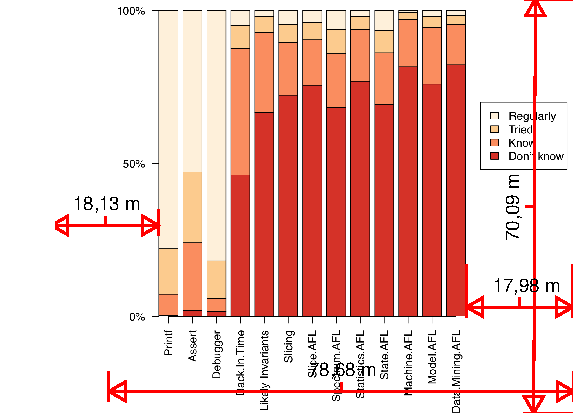
\includegraphics[width=.8\linewidth]{img/tool-usage}
\caption[Answers to "Which debugging tools do you know?"]{Answers to "Which debugging tools do you know?" (from~\cite{perscheid17:studying_the_advancement})}
\label{fig:tool-usage}
\end{figure*}

\section{Do We Need More Debugging Tools?}

Comparing figures \ref{fig:debugging-timeline} and \ref{fig:tool-usage}, we can see that a disconnect between the state of the art in research and the application of debugging in practice began to occur around the 1980s.
Today, we can find a large number of debugging tools, techniques, and prototypes that are very good at what they do, but not widely used by developers.

Consistently with debugging studies, talking to professional software developers we learned that many developers are not even aware that advanced debugging techniques (\ie anything beyond symbolic debugging) exist and may even be available for the programming languages they use.
When developers told us they had heard of an advanced debugging methodology before, they knew not whether respective tools were available for their programming language and were surprised when told that such tools were available.
%If developers know of an advanced debugging tool, they often cited a lack of documentation as the main reason for not using it.
%While locating a software fault, developers don't want to divert attention to learning a new tool.
%\todo{performance issues}

Apparently, developers will not search for new debugging tools while locating a software fault.
But even when better tools are available, switching tools causes an interruption in the thought process that can slow down developers significantly~\cite{altmann14:momentary_interruptions_can_derail}.
Integrating debugging tools directly in the IDE and ensuring they fit the developers' workflow reduces this barrier by improving the accessibility of tools~\cite{wasserman90:tool_integration_in_software, stenning87:on_the_role}.
However, developers still need to know how to use these tools.
Here, it is not enough to expect developers to spend time learning the functionality and features, as "nobody reads documentation"~\cite{rettig91:nobody_reads_documentation} and formal education in debugging is rare~\cite{perscheid17:studying_the_advancement, ballou08:improving_software_quality}.
Instead, the user experience has to be designed such that features can be discovered when needed, without overwhelming the user with too much information and too many options~\cite{brockmann90:the_why_where}.

Thus, instead of only proposing new methods to better locate and repair software faults, 
researchers need to consider the developer as a user of the method, too.
Furthermore, choosing a specific use-case or "niche", instead of developing general purpose debugging tools,
allows to create tools more useful and accessible, at least for the chosen use-case, and further reduce the barriers of entry~\cite{wotawa17:panel_discussion}.

%In the survey by Perscheid et al., developers rated IDE integration and installation less
%important for the adaptation of new debugging tools than ease of use and documentation.
%However, considering 1.2 and what developers told us, it seems that not knowing
%that tools exist is the greatest obstacle.

%These findings show that it is not enough for debugging research to propose new methods
%to better find and repair software faults
%Based on these findings we conclude that 
%Thus, it is not enough for debugging research to propose new methods to better find and fix bugs.
%Having a wide selection of options to tackle a problem is only an advantage if users know how to select the best option and can apply it correctly.
%Thus, researches need to consider the developer as a user of the tool or method, too.
%Debugging tools need to seamlessly integrate into the developer's workflow and tool chain, and allow the exploration of features instead of requiring a formal training of the user.

\section{Millions of Lines of Code to Run a Business}

In our work, we focus on developers of enterprise applications as our target group;
\ie while our results may be useful for developers of other types of applications as well, we consider only problems of developers in this particular field for our design and evaluation.

Enterprise applications, \ie software that supports or automates business pro-\linebreak{}cesses~\cite{fowler02:patterns_of_enterprise_application}, are often large and complex.
\Ac{erp} systems, for instance, have to manage large amounts of business data, interact with many other computer systems, and adhere to complex legal requirements~\cite{linthicum00:enterprise_application_integration}.
SAP’s business suite already consists of several million lines of code~\cite{mallach15:information_systems_what_every}. 
On top of this, optional modules and custom extension are added to provide all required functionality.

The size alone already makes it difficult to locate bugs efficiently.
There is much more code that developers need to understand and the average length of infection chains, the distance between observed failure and responsible code fault, grows accordingly.
On top of that, there is technical complexity that slows down fault localization efforts.

%\begin{figure}
%\centering
%\begin{minipage}{.56\textwidth}
  %\centering
  %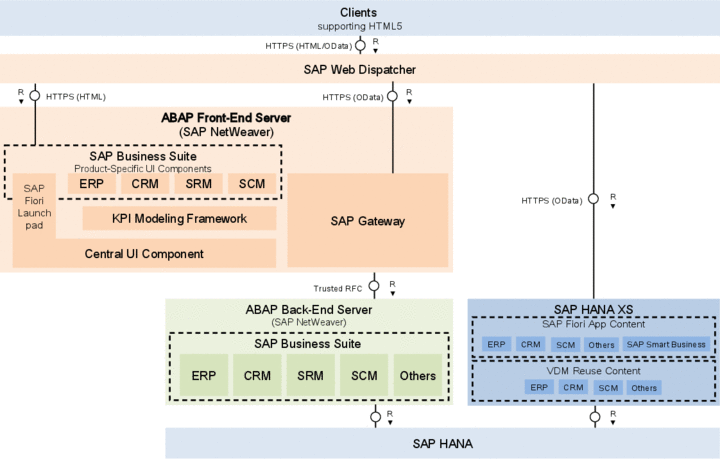
\includegraphics[height=50mm]{img/s4hana}
  %\captionof{figure}[High-level architecture of S/4 HANA]{High-level architecture of an S/4 HANA installation with XS applications~\cite{sap17:setup_of_sap_fiori}\linebreak}
  %\label{fig:s4hana}
%\end{minipage}~~~%
%\begin{minipage}{.42\textwidth}
  %\centering
  %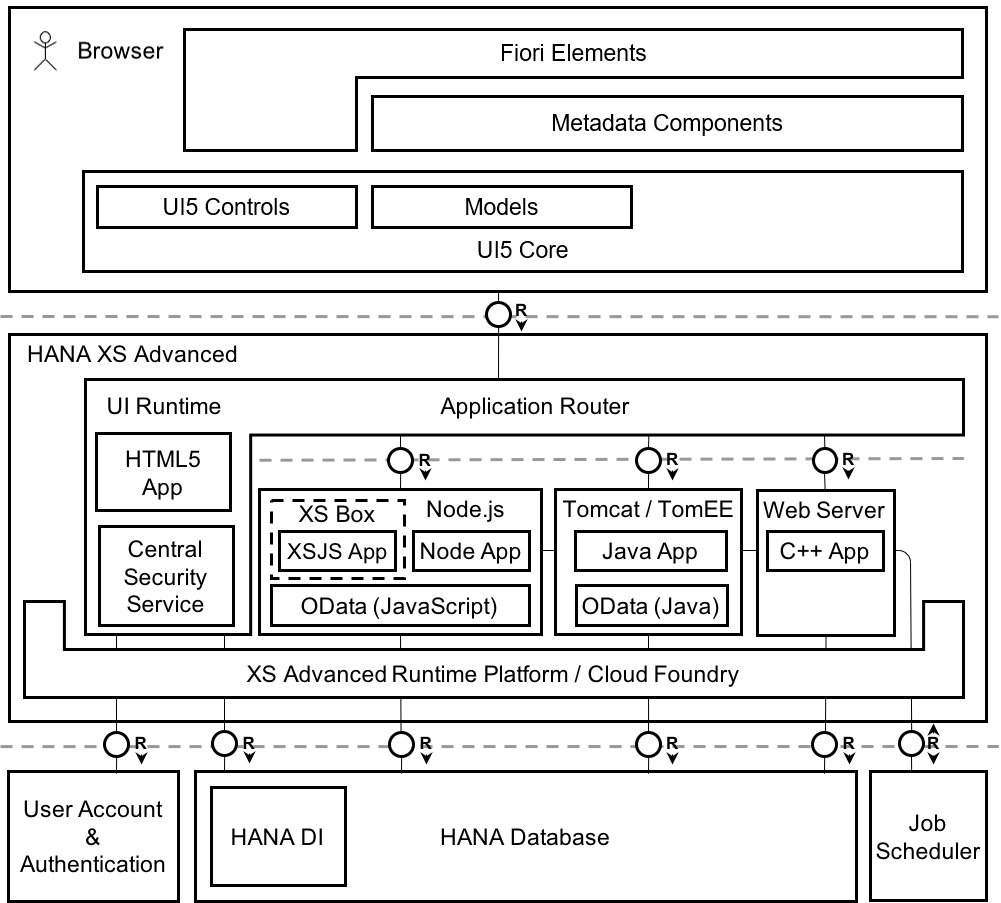
\includegraphics[height=50mm]{img/xsa}
  %\captionof{figure}[Architecture of the SAP HANA XS Advanced framework]{Architecture of the SAP HANA XS Advanced framework~\cite{subatin17:xs_advanced_for_not}}
  %\label{fig:xsa}
%\end{minipage}
%\end{figure}

\begin{figure}
  \centering
  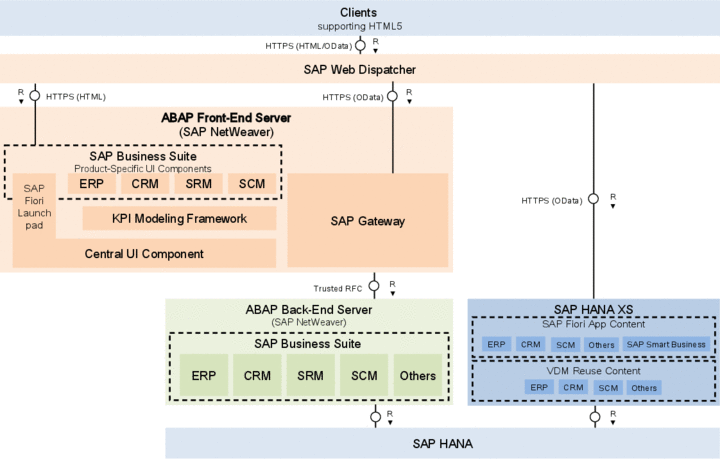
\includegraphics[width=.7\textwidth]{img/s4hana}
  \caption[High-level architecture of S/4 HANA]{High-level architecture of an S/4 HANA installation with XS applications (from~\cite{sap17:setup_of_sap_fiori})}
  \label{fig:s4hana}
\end{figure}


\Cref{fig:s4hana} shows the high-level architecture of SAP's business suite "S/4 HANA" from a technical perspective. 
On the left, the two major components, the ABAP front-end and back-end servers, contain the majority of business logic.
User clients, shown at the top, interact with the system using a browser with HTML5 support or the SAP GUI.
At the bottom of the stack, the SAP HANA database stores and manages application data.
On the right, additional reporting and analytics applications run in the SAP HANA Extended application Services (XS) Advanced framework.
Each product of the business suite, such as the ERP or CRM system, can add modules to all components in this architecture.

\begin{figure}
  \centering
  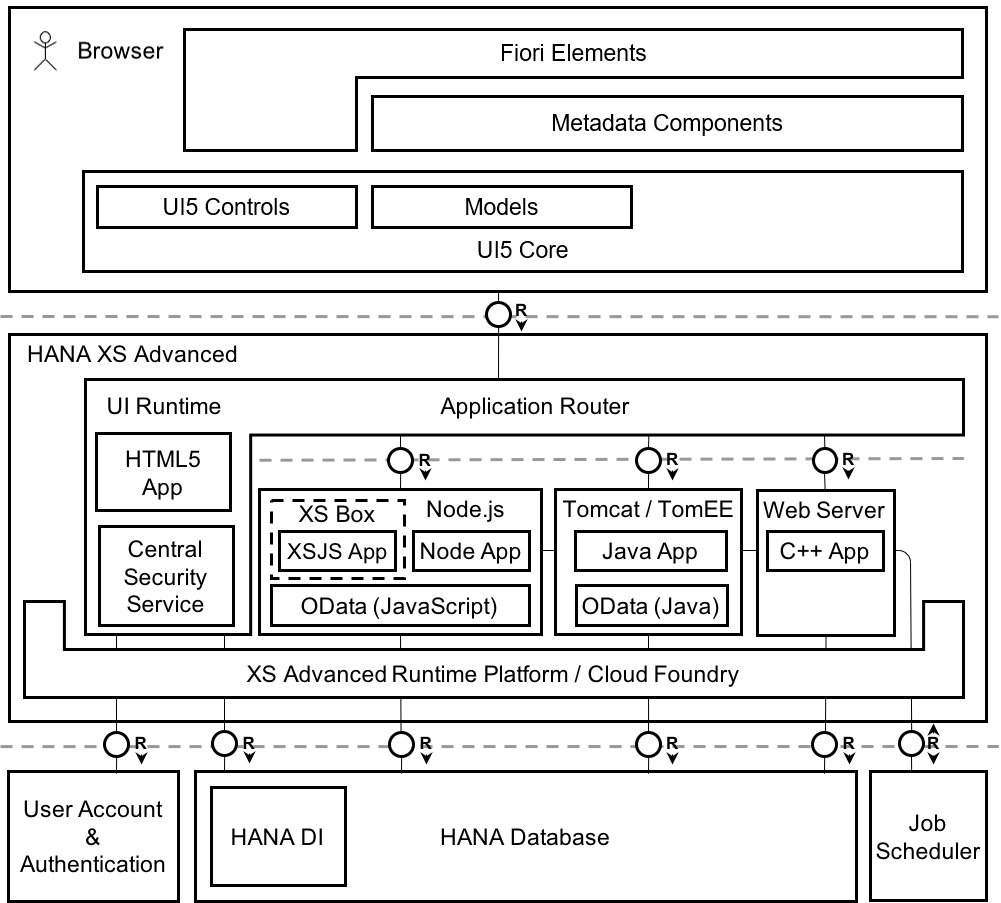
\includegraphics[width=.5\textwidth]{img/xsa}
  \captionof{figure}[Architecture of the SAP HANA XS Advanced framework]{Architecture of the SAP HANA XS Advanced framework (from~\cite{subatin17:xs_advanced_for_not})}
  \label{fig:xsa}
\end{figure}

The architecture of the XS Advanced framework is shown in more detail in~\cref{fig:xsa}.
Again, we find a browser-based client with a JavaScript UI library at the top and the SAP HANA database at the bottom.
In the center, the XS Advanced application framework supports server-side applications written in JavaScript, Java, or C++.
The dashed lines indicate communication across execution environment boundaries.

%Complex software systems often consist of multiple interoperating components written in different programming languages and running in different environments.
Both architectures match the three-tier application pattern~\cite{fowler02:patterns_of_enterprise_application}:
A database layer handles persistence and data-intensive computations.
On top, the application layer implements most of the business process logic and acts as a gateway to the client.
In the client, the user interface layer provides a rich user experience and sends requests to the application back-end to trigger actions and obtain data.
Because of the heterogeneous technologies, each layer typically comes with its own tool set and no tool can be used to work on all layers at once.

%Bugs can occur in any layer but often manifest themselves as failures in the user interface.
%Thus, developers first have to guess in which layer the error originated before choosing the appropriate debugging tool for that layer.
%If the guess turns out to be wrong, developers have to switch tools and context before continuing the bug hunt.
%Locating bugs in the interaction between two layers becomes even more difficult, as developers may have to switch tools several times to understand the fault.

%As these diagrams illustrate, enterprise applications consist of multiple interoperating components written in different programming languages and running in different environments.
Software faults can occur in any component but often manifest themselves as failures in the user interface.
Thus, developers first have to guess in which component the error originated before choosing the appropriate debugging tool for that component.
If the guess turns out to be wrong, developers have to switch tools and context before continuing the bug hunt.

To demonstrate the difficulty of localizing faults in complex systems, \cref{fig:worstcase} shows an example that is close to a worst-case scenario based on the S/4 HANA architecture.
A fault in the ABAP Front-End server causes corrupted data to be passed down into the database.
Later, the data is retrieved by an XSA application and causes a failure in the client.
Dashed lines indicate boundaries of execution environments.
As can be seen, to follow the infection chain from the failure to the fault, developers would have to switch debugging tools six times.

\begin{figure*}[t]
\centering
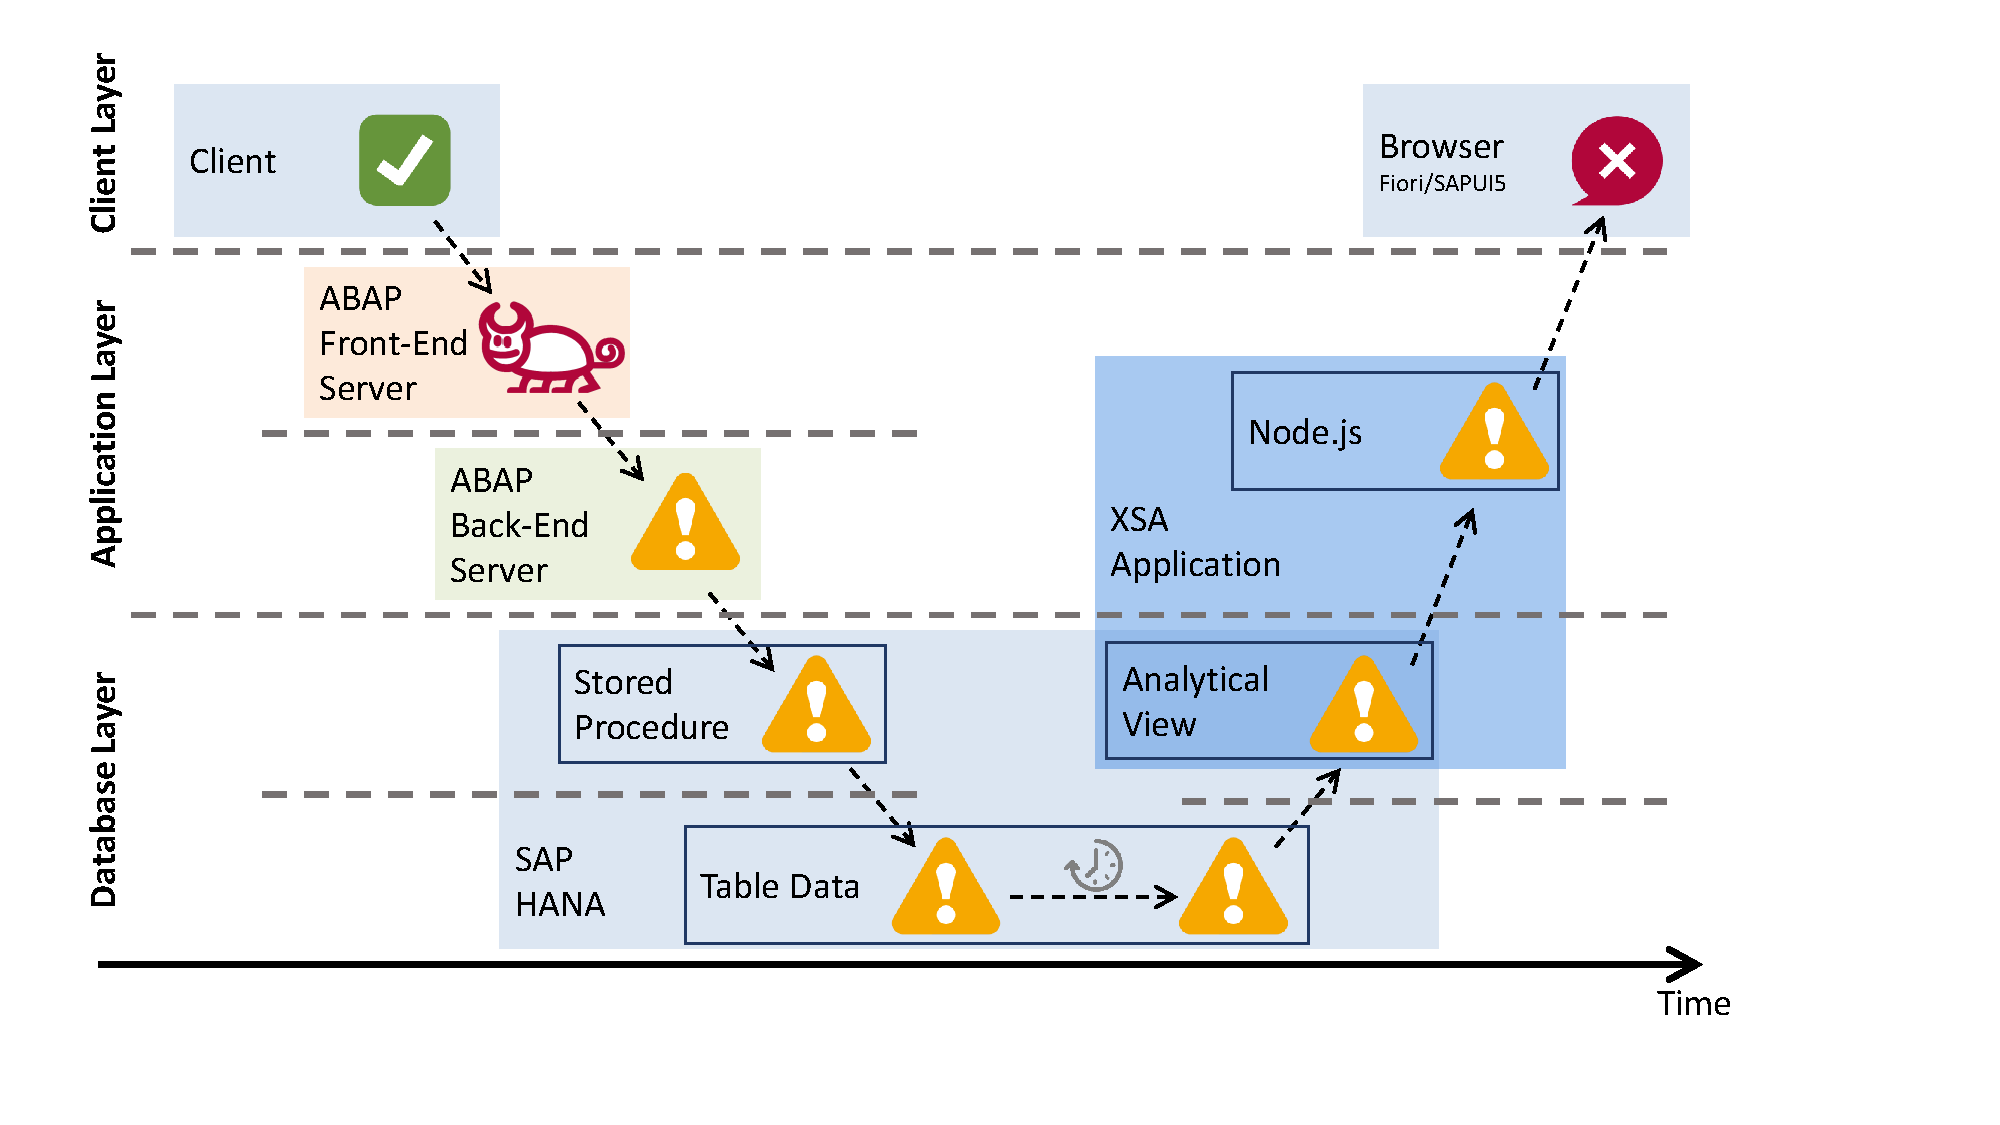
\includegraphics[width=.9\linewidth]{img/worstcase}
\caption{An infection chain crossing several runtime environments}
\label{fig:worstcase}
\end{figure*}

Locating faults in the interaction between two components becomes even more difficult, as developers may have to switch tools back and forth repeatedly to understand the fault.
To efficiently debug a multi-tier application, developers would need a single debugger that is not only capable of debugging each layer but also aware of the interaction between layers at a meaningful level of abstraction.
Additionally, the debugger needs to provide help
navigating the large amounts of code that a long infection chain passes through
and consider database tables as part of the program state.

%Furthermore, the debugger needs to include the database
%Finally, to help developers handle the complexity and size of an enterprise application, the debugger should provide analysis features that integrate in the debugging process, instead of interrupting it.

%Looking back at the history of debugging, we find that innovations in debugging were usually quickly adopted when they occurred alongside changes in how software was developed.
%Recent trends in database technology and software engineering practices fundamentally affect how enterprise applications will be developed in the future~\cite{plattner15:the_in-memory_revolution_how}.
%We looked at these trends to identify specific problems today's developers have to face when debugging their code that can not be adequately solved with existing tools. 

\section{Our Approach} %(Research Questions \& Contributions) Our Approach

%\newcommand{\RQ}[1]{\paragraph{\emph{#1}}}
\newcommand{\RQ}[1]{\subsection*{\textsl{#1}}}

The overarching motivation of this work is to reduce the time and effort needed to locate faults in multi-tier enterprise applications.
In the past decades, many advanced debugging techniques have been developed that are not widely used in practice for various reasons.
Omniscient debugging, for instance, can significantly improve fault localization, but imposes a large overhead on run-time and memory cost.
By adapting omniscient debugging specifically to the needs of enterprise application developers,
while also keeping an eye on overhead and usability, we expect to increase the usefulness and accessibility of this approach, making it more appealing in practice.

Looking back at the history of debugging, we find that innovations in debugging were usually quickly adopted when they occurred alongside changes in how software was developed.
Recent trends in database technology and software engineering practices fundamentally affect how enterprise applications will be developed in the future~\cite{plattner15:the_in-memory_revolution_how}.
%We looked at these trends to identify specific problems today's developers have to face when debugging their code that can not be adequately solved with existing tools. 
%Looking at these trends, 
Confirming previous studies~\cite{eisenstadt97:my_hairiest_bug_war, perscheid17:studying_the_advancement}, our research (cf. \cref{sec:enterprise_applications}\todo{cite}) has shown that much hardship for developers debugging enterprise applications is caused by long infection chains that cross boundaries of execution environments.
From this insight, we derived our research question:
%Thus, we defined the following research question:

\medskip
\noindent
\emph{How can we adapt omniscient debugging to reduce the time and effort needed to track long infection chains in multi-tier enterprise applications?}
%\blockquote{How can advanced debugging techniques be adapted to reduce the time and effort needed to track long infection chains across sub-system boundaries in multi-tier enterprise applications?}
\medskip

\noindent
Developers will be reluctant to use tools if the required costs outweigh the expected benefits.
However, the longer the infection chain, the more of a difference \acfp{odb} can make.
We identified three areas were current omniscient debugging tools do not meet the needs of developers of enterprise applications.

%\RQ{Contribution 1: A method for the faster navigation of long infection chains}

%When developers debug a program, they are typically not just "browsing" the execution, but rather searching for something specific.
%In particular, when tracking an infection chain the most common operation is to find the origin of a potentially erroneous value.
%In large and complex systems, infection chains tend to be very long as well.
%Thus, if a debugging tool can increase the speed with which developers can track infection chains, the overall time needed to locate a bug can be reduced.

%The debugger's vast knowledge about the execution can be used for dynamic analyzes.

\bigskip\noindent
\emph{Interactive Dynamic Slicing} is a new debugging workflow that addresses the need to track long infection chains through large amounts of code.
Generally, there are two major approaches to fault localization: manual debugging, \eg using \acp{odb}, and \acf{afl}.
\Acp{odb} make it easier to freely navigate a program execution, but offer no specific help for tracking down relevant code locations.
Many \ac{afl} techniques, on the other hand, can identify code locations likely related to a failure, but do not provide a way to verify this relation.
Furthermore, the accuracy of \ac{afl} diminishes over longer distances.
Combining both approaches, however, keeps their advantages while reducing their drawbacks.

The execution history available to the \ac{odb} can be used to quickly compute dynamic slices to help developers to identify relevant code.
With Interactive Dynamic Slicing, while debugging the dynamic slice, at any point developers can add or adjust the slicing criteria.
A new slicing algorithm allows for incremental configuration of a slice. 
This way changes are applied instantly, without interrupting the debug session. 
A new UI component, the \emph{Slice Navigator}, provides a unique view on the execution by combining relevant information from both the \ac{odb} and the slicing subsystem.

\bigskip\noindent

%\RQ{Contribution 2: Back-in-time debugging on the database layer}

%\emph{TARDISP} is a debugger that brings back-in-time debugging down to the database layer.
Enterprise applications are very data-driven.
Developers need direct access to the database not only to understand the context and evaluate the correctness of an operation, but the data itself, with erroneous or unexpected values, can be the source of software failures.
In such cases, developers must not only identify the responsible data records, but also determine how they found their way into the database.

%With back-in-time debuggers, developers can explore what happened before observable failures by following infection chains back to their root causes. 
Again, \acp{odb} can help with this task, but
while there are several such debuggers for object-oriented programming languages, we do not know of any debuggers with back-in-time capabilities at the database-level.
Thus, if failures are caused by components that interact with the database, developers have difficulties in understanding their unexpected behavior.

%We developed an approach for bringing back-in-time debugging down to the database.
%Our \emph{TARDISP} debugger allows developers to step queries backwards and inspecting the database at previous and arbitrary points in time. 
\emph{TARDISP} is a debugger that brings back-in-time debugging down to the database layer.
We developed an approach allowing developers to step backwards in database programs, re-execute queries and inspect the database at previous and arbitrary points in time.
With the help of an \emph{Back-in-time SQL}, developers can express queries covering a period of execution time within a debugging session and handle large amounts of data with low overhead on performance and memory. 
%The entire approach has been evaluated within a development project at SAP and shows promising results with respect to the gathered developer feedback.

%\RQ{Contribution 3: Seamless omniscient debugging across the layers of a 3-tier architecture}
\bigskip\noindent

%The \emph{TARDISP full stack debugger} extends TARDISP to aggregate traces from multiple concurrent executions into one continuous debug session.
Even with back-in-time debugging available in every layer of the software stack, developers still have to switch tools when following an infection chain along requests between sub-systems.
Switching tools imposes a significant cognitive overhead on developers and can break their productive flow.

We extended TARDISP into a \emph{full stack debugger} by aggregating traces from multiple concurrent executions into one continuous debug session.
Assuming back-in-time debugging capabilities for each individual application tier, 
we introduce hierarchical step numbering based on synchronization points between components to create a partial ordering of instructions in all concurrent executions.
A visualization in the front-end shows developers which UI element is affected by which back-end operation, providing them with a top-down summary of the execution.
A second visualization is shown in the debugger and helps developers to navigate the application flow.

%\section{Contributions} 
%summarize again \\ \\
%1) Interactive dynamic slicing combines AFL and ODB \\
%- new slicing algorithm \\
%- Slice navigator UI\\
%\\
%2) BiT down to the database\\
%- model for re-executing queries\\
%- SQL extension\\
%\\
%3) system debugger\\
%- unified model\\
%- top-down view\\


%% improve debugging;  
%This challenge will be approached from two directions.
%First, recent debugging innovations need to be made more available in practice.
%It is not enough to simply make more features available in debugging tools, the features need to be conveniently accessible and the cost of learning a new feature must not be too high at any point in time.
%Second, debugging tools need to move along with recent technology trends.
%Developers need better support debugging applications that handle large amounts of data and are composed of sub-systems with heterogeneous technology stacks.
%From this, we defined three research questions.
%
%% mtiier verbessern ; verfolgen
%
%\RQ{Research Question 1: How can debuggers help developers to navigate a program when following a long infection chain?}
%
%When developers debug a program, they are typically not just "browsing" the execution, but rather searching for something specific.
%In particular, when tracking an infection chain the most common operation is to find the origin of a potentially erroneous value.
%In large and complex systems, infection chains tend to be very long as well.
%Thus, if a debugging tool can increase the speed with which developers can track infection chains, the overall time needed to locate a bug can be reduced.
%
%There are two major approaches to fault localization: manual debugging, \eg using \acfp{odb}, and \acf{afl}.
%\Acp{odb} make it easier to freely navigate a program execution, but offer no specific help for tracking down relevant code locations.
%Many \ac{afl} techniques, on the other hand, can identify code locations likely related to a failure, but do not provide a way to verify this relation.
%Furthermore, the accuracy of \ac{afl} diminishes over longer distances.
%By combining both approaches, however, we believe we can keep their advantage while reducing their drawbacks.
%%The debugger's vast knowledge about the execution can be used for dynamic analyzes.
%
%We developed \emph{interactive dynamic slicing}, a new debugging workflow that combines omniscient debugging and dynamic slicing. 
%The execution history available to the \ac{odb} can be used to quickly compute dynamic slices to help developers to identify relevant code.
%While debugging the dynamic slice, at any point developers can add or adjust the slicing criteria.
%A new slicing algorithm allows for incremental configuration of a slice. 
%This way changes are applied instantly, without interrupting the debug session. 
%A new UI component, the \emph{Slice Navigator}, provides a unique view on the execution by combining relevant information from both the \ac{odb} and the slicing subsystem.
%
%\RQ{Research Question 2: How can programs handling large amounts of data be debugged and analyzed efficiently?}
%
%Enterprise applications are very data-driven.
%Developers need direct access to the database not only to understand the context and evaluate the correctness of an operation, but the data itself, with erroneous or unexpected values, can be the source of software failures.
%In such cases, developers must not only identify the responsible data records, but also determine how they found their way into the database.
%
%With back-in-time debuggers, developers can explore what happened before observable failures by following infection chains back to their root causes. 
%While there are several such debuggers for object-oriented programming languages, we do not know of any back-in-time capabilities at the database-level.
%Thus, if failures are caused by components that interact with the database, developers have difficulties in understanding their unexpected behavior.
%
%We developed an approach for bringing back-in-time debugging down to the database.
%Our \emph{TARDISP} debugger allows developers to step queries backwards and inspecting the database at previous and arbitrary points in time. 
%With the help of a SQL extension, developers can express queries covering a period of execution time within a debugging session and handle large amounts of data with low overhead on performance and memory. 
%The entire approach has been evaluated within a development project at SAP and shows promising results with respect to the gathered developer feedback.
%
%\RQ{Research Question 3: How can developers debug complex systems without being impeded by control-flow crossing sub-system boundaries?}
%
%Even with back-in-time debugging available in every layer of the software stack, developers still have to switch tools when following an infection chain along requests between sub-systems.
%Switching tools imposes a significant cognitive overhead on developers and can break their productive flow.
%
%Assuming back-in-time debugging capabilities for each application tier, 
%we extended TARDISP to aggregate traces from multiple concurrent executions into one continuous debug session.
%We introduce hierarchical step numbering based on synchronization points between components to create a partial ordering of instructions in all concurrent executions.
%A visualization in the front-end shows developers which UI element is affected by which back-end operation, providing them with a top-down summary of the execution.
%A second visualization is shown in the debugger and helps developers to navigate the application flow.

\section{Outline}

The remainder of this thesis is structured as follows:

\Cref{sec:debugging_in_ea} provides background on our work.
We describe the process which developers typically use to locate faults with a debugger, how it changes with back-in-time debugging.
Furthermore, we outline the typical components of an enterprise application and how debugging is affected by recent changes in technology.

In \cref{sec:ids}, we present interactive dynamic slicing, a new debugging workflow that combines omniscient debugging with dynamic slicing.
A new slicing algorithm allows developers to incrementally change a slice. 
The Slice Navigator, a novel GUI component, combines access to the debugger and the slicer in a single view.
With a user study, we show that our approach allows for more efficient fault localization, even for developers that are not yet familiar with the tools.

\Cref{sec:db_odb} focuses on back-in-time debugging in the database.
We present an approach to efficiently trace and replay the execution of programs handling large amounts of data,
an SQL extension allowing developers to query past data and filter for changes between points in time,
and a prototype implementation of our approach.
%a prototype implementation to database developers and gathered valuable feedback that confirms the usefulness of our approach.

In \cref{sec:stack_odb}, we describe a model for hierarchical omniscient debugging of concurrent executions and propose visualizations that can help developers to navigate control flow in a multi-tier application.

In \cref{sec:relatedwork}, we discuss related work in the area of back-in-time debugging, slicing, and analysis of enterprise applications.

\Cref{sec:conclusion} suggests areas for improvement and future work and concludes.


%How can debugging be improved to reduce the time needed to find a bug?
%\\- How can developers efficiently navigate a program execution?
%\\- How can the debugger help to identify relevant code?
%\\- How can programs handling large amounts of data be debugged and analyzed efficiently?
%
%A better way to track failure causes
%\\- Improved existing program analysis technique 
%\\- Seamless integration into debugging workflow
%\\- Allows more efficient debugging by increasing focus, providing more relevant information, and reducing tool-related interruptions
%
%Efficient omniscient debugging in the database
%\\- Fully featured ODB with little overhead on performance and memory
%\\- Query past database states
%\\- Query changes in the database



\chapter{Debugging in Enterprise Applications}
\label{sec:debugging_in_ea}

Debugging is the process of finding and resolving defects in a computer program~\cite{araki91:a_general_framework}.
Efficient debugging requires a good understanding of the program and the ability to distinguish correct and incorrect program behavior, i.e., some external knowledge about the program's requirements.
Accordingly, debugging tools can assist developers by identifying relevant code locations for review, by analyzing and visualizing program behavior, and by suggesting fixes.
% knowledge: I. Vessey. Expertise in Debugging Computer Programs: A Process Analysis

In this chapter, we present approaches to debugging that built the foundation of our work and discuss specific challenges in the context of enterprise applications.

%\section{How To Debug a Program}
\section{The Scientific Approach to Fault Localization}

% Experienced developers are able to locate defects up to three times faster and add fewer new failures than novices
% J. Gould. Some Psychological Evidence on How People Debug Computer Programs.

% novices add more errors
% L. Gugerty and G. Olson. Comprehension Differences in Debugging by Skilled and Novice Programmers.
The starting point for a debugging task is a known program failure, an observed deviation from correct program behavior.
Developers with only little debugging experience often debug with an incomplete understanding of the program, modifying the code until the failure can no longer be reproduced~\cite{gugerty86:comprehension_differences_in_debugging}.
These modifications may be based on educated guesses but otherwise follow no particular strategy.
While this trial-and-error based approach usually works for simple bugs, it has several critical drawbacks.

Firstly, there is a significant risk of introducing additional bugs into the system~\cite{gugerty86:comprehension_differences_in_debugging,yin11:how_do_fixes_become}, especially when developers fail to consider the side-effects of their changes or incorrectly undo wrong guesses.
Most importantly, however, this method can not be used to approach more complex bugs effectively.
Some bugs need fixes at multiple code locations or have a large conceptual distance between the observed failure and the defect in the code.
In such cases, developers risk entirely missing the root cause of the problem~\cite{gu10:has_the_bug_really},
\ie while they may succeed in fixing one of its symptoms, the actual bug remains in the system.
To overcome these problems, developers need a more structured approach to debugging, one that separates localizing and fixing the fault.

Experienced developers often follow a process that is similar to the scientific method~\cite{araki91:a_general_framework}.
\Cref{fig:scientifiy-method} shows the process as a flow chart.
First, developers formulate a hypothesis explaining the failure; then, they attempt to verify the hypothesis through an experiment. 
\begin{figure*}[t]
\centering
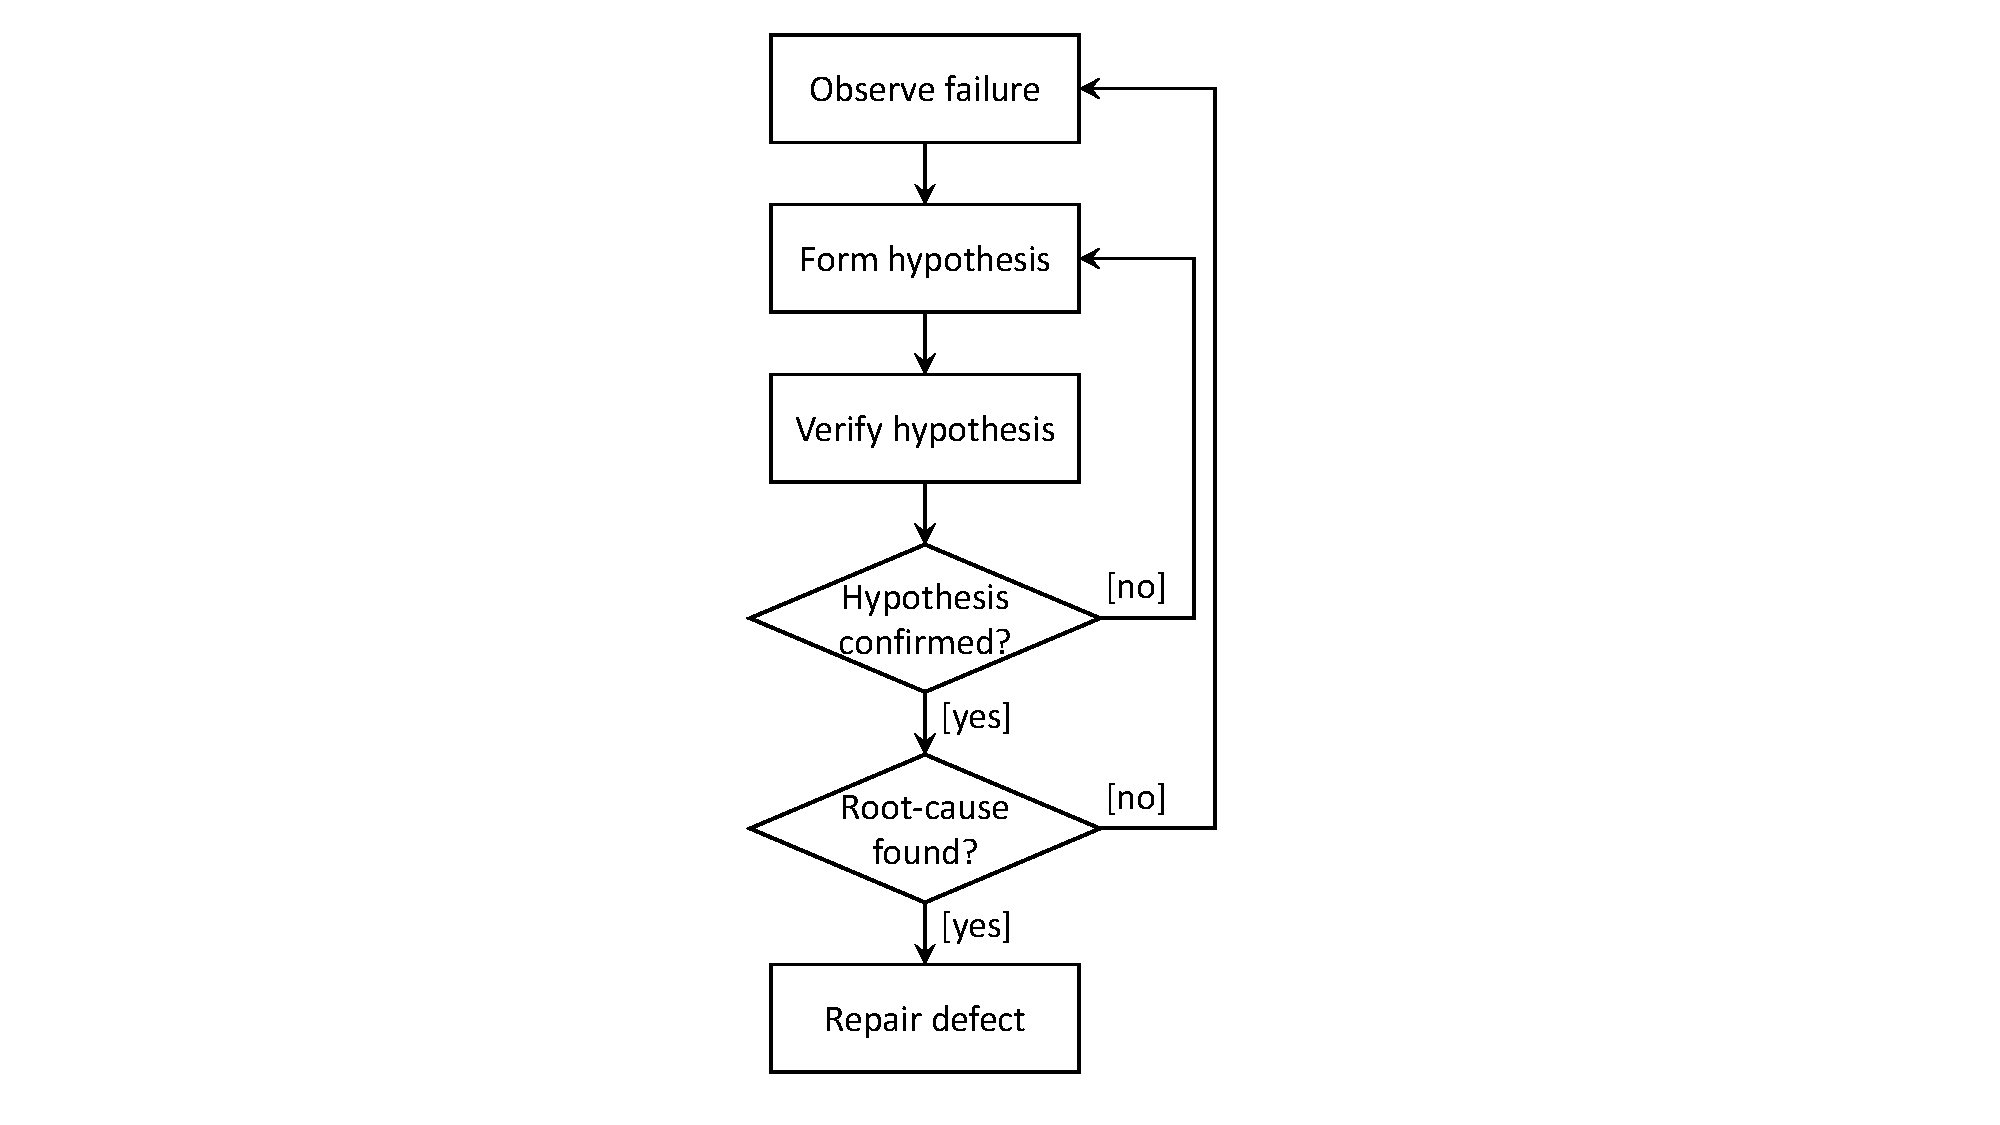
\includegraphics[width=.4\linewidth]{img/workflow-scientific-method}
\caption{The scientific approach to fault localization.}
\label{fig:scientifiy-method}
% R. Metzger. Debugging by Thinking - A Multidisciplinary approach.
\end{figure*}
If the experiment does not confirm the hypothesis, developers must improve their understanding of the program in order to form a better one.
If the experiment confirms the hypothesis, however, it has not necessarily revealed the root cause of the failure.
Sometimes, the hypothesis is to vague and the problem needs to be narrowed down further.
In other cases, the experiment revealed that the erroneous behavior of one component was caused by incorrect input of another component, in which case a new failure cause becomes the focus of investigation.
Either way, developers repeat the hypothesis-experiment cycle until they identify the root cause and can begin the repair.

\section{Back-in-Time and Omniscient Debugging}
\label{sec:omni-debugging}

Very often, defective code does not cause the program to fail immediately.
Instead, it creates an error in the program state that propagates, in accordance to the garbage-in-garbage-out principle, until it yields to a failure in a different part of the application.
This sequence of erroneous states is also called the infection chain~\cite{zeller09:why_programs_fail}.
Developers tasked to locate the defect have to follow the infection chain backwards through execution time.

%Tools can support the fault localization process 

\begin{figure*}[t]
\centering
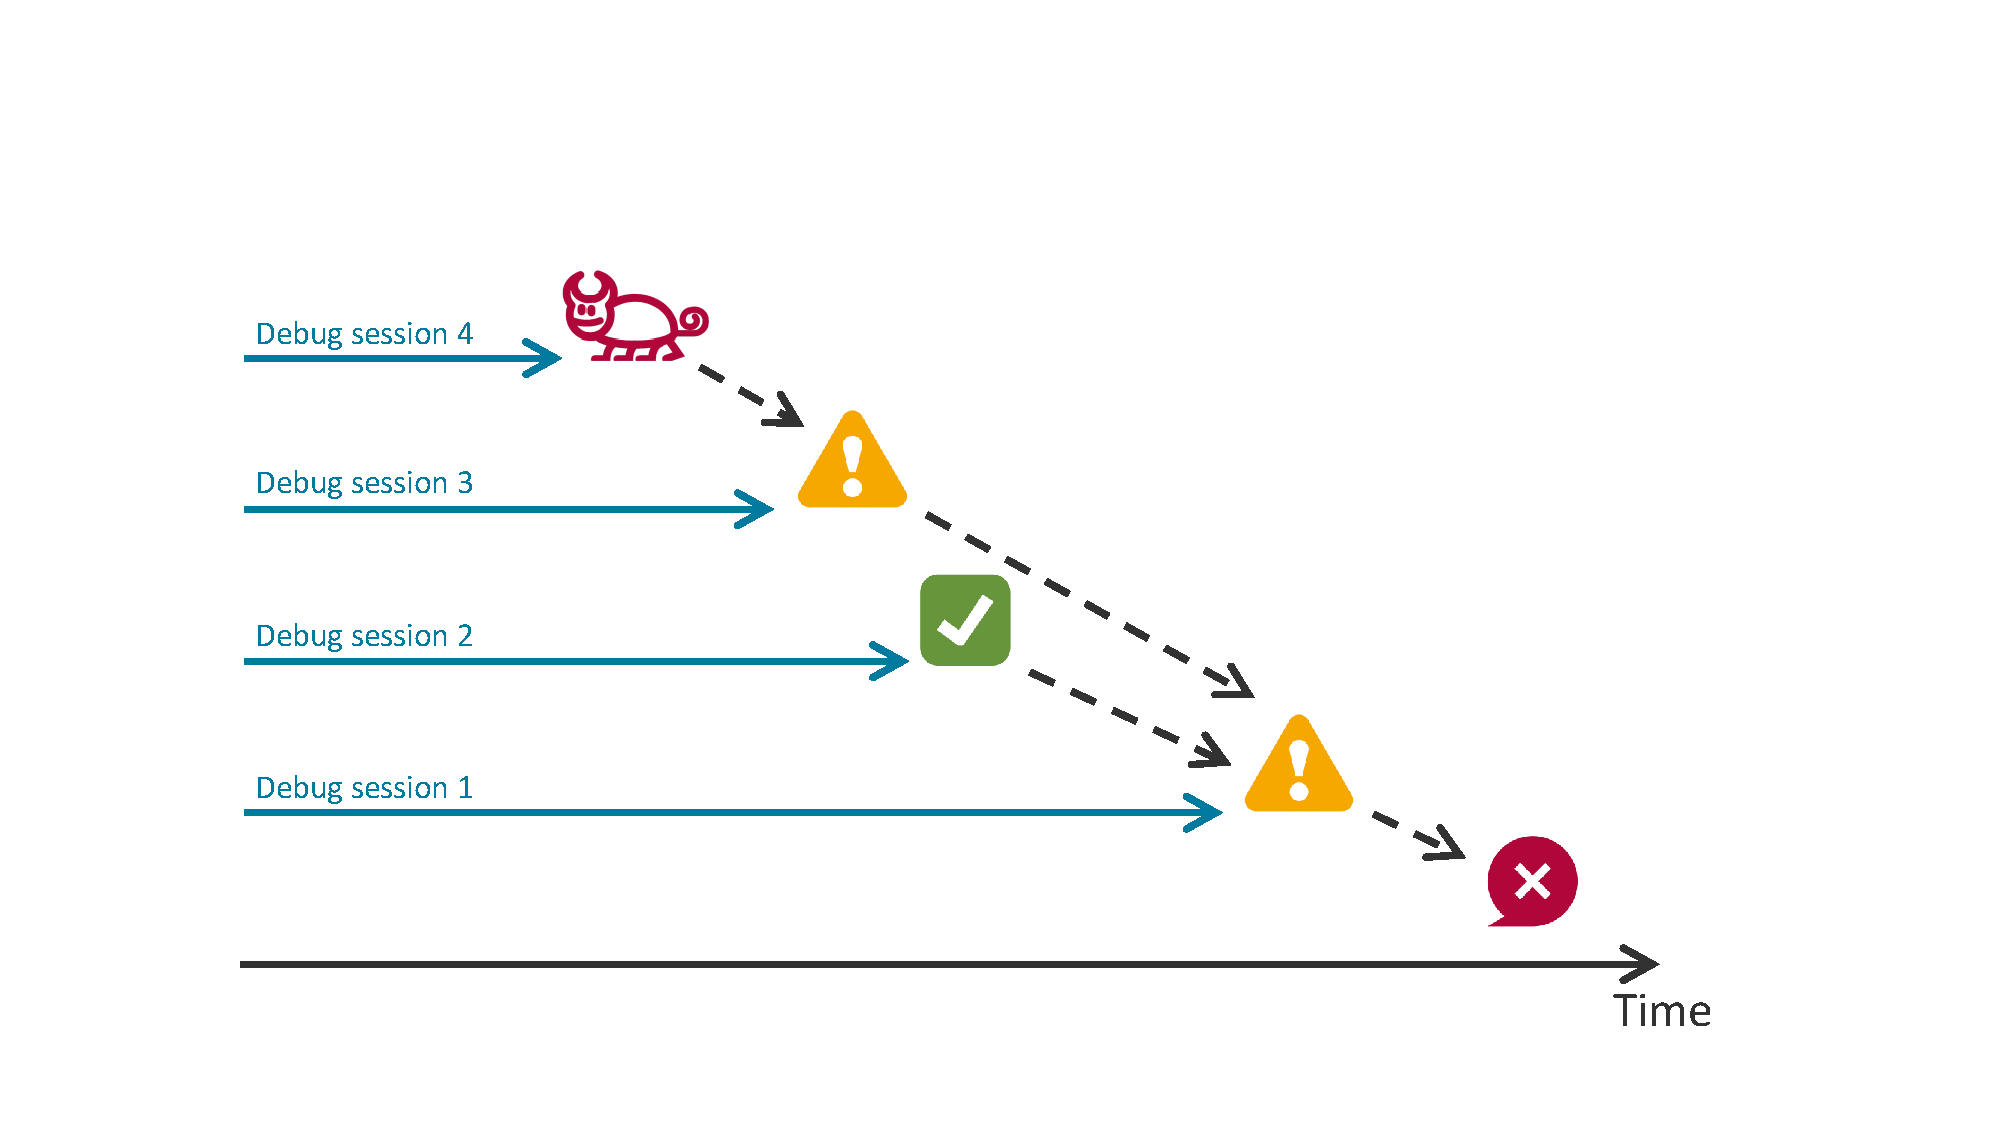
\includegraphics[width=.9\linewidth]{img/workflow-traditional}
\caption{Following an infection chain with a debugger.}
\label{fig:workflow-traditional}
\end{figure*}

\Cref{fig:workflow-traditional} shows how developers track an infection chain with a debugger.
Beginning at the failure, developers follow the infection chain backwards through execution time.
Each step consists of forming a hypothesis and confirming it by inspecting the relevant code location with a debugger. \todo{explain image in more detail}
Following this method, developers will continually get closer to the root cause of the bug.
If developers have not enough knowledge of the program to identify relevant code locations for the next step, the debugger can also be used to explore the program execution to find suspicious locations.
Thus, debuggers can help developers with both tasks in the scientific debugging approach.

However, debuggers have one major limitation: they do not allow developers to go back.
Developers track the infection chain backwards through time.
As \cref{fig:workflow-traditional} shows, to move backwards a new debug session has to be started at every step.
Likewise, when using a debugger to explore an execution, developers might accidentally step over a method instead of stepping into it, either because they did not expect relevant behavior to occur inside that method or simply because of pressing the wrong button.
In both cases, the debug session has to be restarted to get back in time.

Restarting the debugger is usually an easy task, and getting to the desired point in the execution can be as simple as setting a breakpoint at the respective location.
Alas, often getting to the right point is more cumbersome.
For instance, it may happen that the breakpoint is hit multiple times.
In this case developers have to either resume the execution repeatedly until the right point in time is reached, or set a breakpoint at a different location that is hit less often and manually step from there.
Either way demands high concentration from the developer as making a mistake means having to start all over again.
In other cases manual interaction with the program is required to set up the program state in which the error will occur.
This, too, has to be repeated with every restart of the debug session.
Thus, while restarting the debugger is in the best case a simple operation that imposes only a small delay on the developer, it often is a complex task that requires careful attention.
This attention is then drawn away from solving the actual problem.

\begin{figure*}[t]
\centering
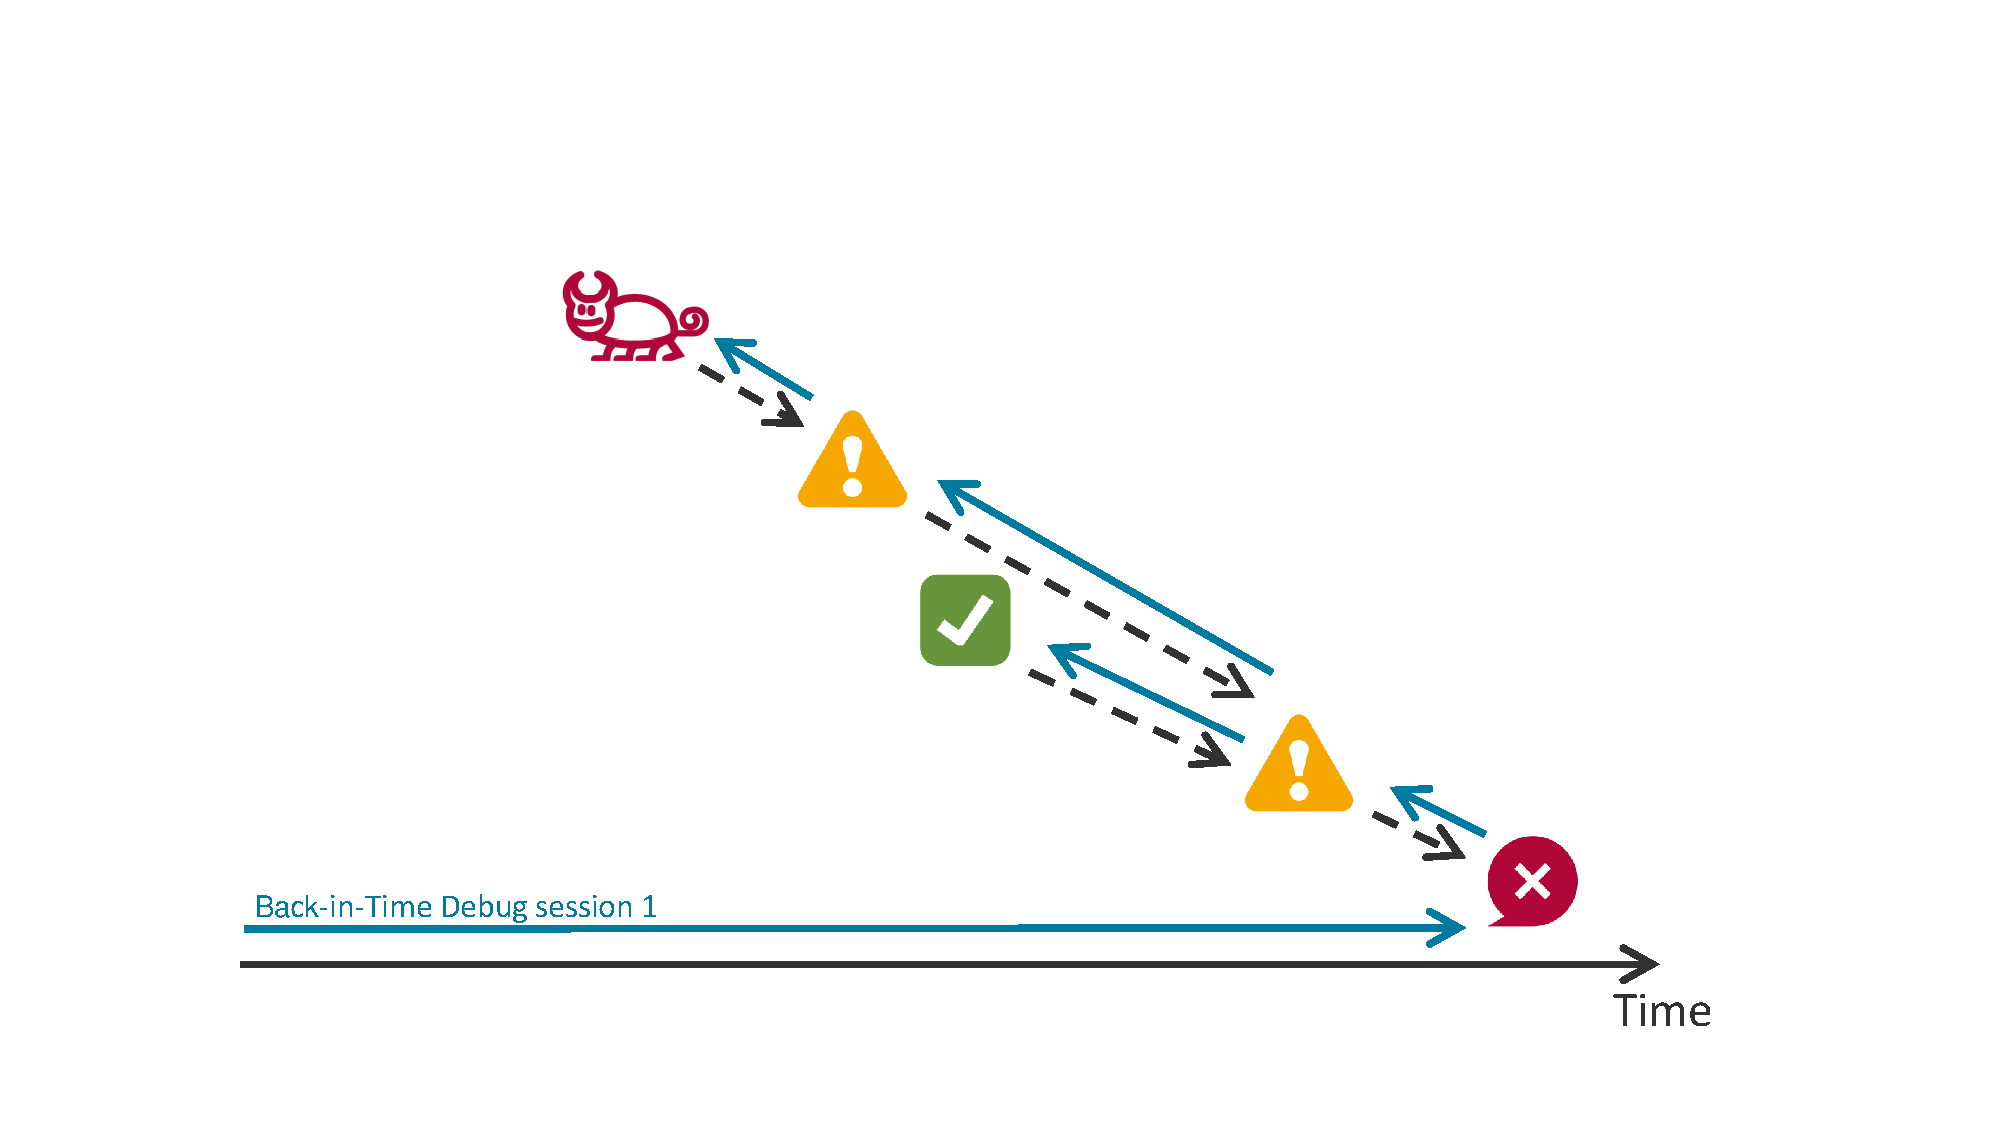
\includegraphics[width=.9\linewidth]{img/workflow-odb}
\caption{Following an infection chain with a back-in-time debugger.}
\label{fig:workflow-odb}
\end{figure*}

%%---------
\emph{Back-in-time debuggers} seek to remedy this problem by allowing developers to step backwards.
This all but removes the need to restart the debugger.
\Cref{fig:workflow-odb} shows how developers track the infection chain with a back-in-time debugger.
Instead of restarting at every step, developers move back and forth along the data-flow, thereby reducing the time needed for each hypothesis-confirmation cycle.

Different approaches exist to realize back-in-time debugging.
Recording lost state allows the debugger to roll back changes by reversing each instruction~\cite{feldman88:igor_a_system,cook02:reverse_execution_of_java,lieberman95:zstep_95_a_reversible}.
By creating regular snapshots of the entire program state, the debugger can go back faster over longer distances in time~\cite{boothe00:efficient_algorithms_for_bidirectional,tolmach93:a_debugger_for_standard}.
% TODO: about IO
%%----
Many different strategies can be used to realize back-in-time capabilities in a debugger.
These strategies come with different trade-offs between overhead and usefulness.

\todo{why regular debuggers again?}
With a regular debugger, the only way to go back in time is to restart the execution.
Tools can be used to automate this approach, but some manual effort is often required to get to a specific point in time.
The clumsiness of this approach is what motivated research in back-in-time debuggers in the first place.
On top of that, this approach only works when the execution is deterministic and does not depend on external factors, such as resources or timing.
Some debuggers even allow to restart executions at the method level.
This greatly improves the usability when developers want to re-examine the program flow, but as state changes are not reverted executing a method multiple times can have unintended side-effects.

To improve determinism when re-executing code, snapshot-based debuggers record the program memory at regular intervals~\cite{feldman88:igor_a_system, boothe00:efficient_algorithms_for_bidirectional}.
%%----

A special kind of back-in-time debugger, called \emph{omniscient debugger}, keeps a record of all state changes in the execution history~\cite{lewis03:debugging_backwards_in_time}.
This not only allows developers to step backwards in time, it also opens the possibility to run structured queries on the history of program states.
For example, an omniscient debugger can easily list all invocations of a method or show a history of all field accesses in an object.
Such information can be very helpful for developers trying to understand a program and is not easily obtainable through other means.

Recording the entire execution history also allows the debugger to run \emph{post-mortem}, i.e., it simulates an active debug session while the actual program has already terminated.
This way, developers can not only restart the debugger later without having to re-run the program, but they can do so on a different machine or even share the recording with coworkers.
\todo{about memory usage}


%\subsection{Slicing}
\section{The Evolution of Slicing Algorithms}
\label{sec:evolution_of_slicing}

A different way how tools can support the debugging process is by helping to form hypotheses about the failure.
Better hypotheses reduce the number of iterations needed in the hypothesis-confirmation cycle and thereby shorten the time needed to locate a bug.
While developers first need to improve their understanding of the program in order to form better hypotheses, a tool can quickly analyze large parts of a program or program execution and suggest likely causes for a fault.
This approach is called \emph{automatic fault localization} and many techniques to locate suspicious code have been developed~\cite{wong16:a_survey_on_software}.
In our work, we build on one of these techniques, called "slicing".

Research has shown that developers also break programs down into pieces of code that are related by data flow~\cite{weiser82:programmers_use_slices_when}.
Such "slices" are often not contiguous and can contain code from many different parts of an application, increasing the navigation overhead for developers trying to understand the program.
Here, tools can help to identify related statements, saving time and reducing the mental overhead for developers.

In 1981, Weiser introduced slicing as a technique helping developers to find related code for a given question~\cite{weiser81:program_slicing}.
According to Weiser, a slice is a subset of a program that, when executed, yields the same state trajectory with respect to given slicing criteria as the original program would have.
The slicing criteria are pairs of variables and code locations.
An important property of the resulting slice is that it must be executable.
This allows the slice to be compiled and inspected with a debugger.

Weiser proposed an algorithm for computing static slices, i.e., slices that are correct for every possible input of the program.
Static slices often are very large, especially for complex applications, and many sophisticated methods have been developed to reduce the size of static slices~\cite{ottenstein84:the_program_dependence_graph, lyle93:program_slicing_in, hoffner95:evaluation_and_comparison}.

In 1988, Korel and Laski proposed to compute slices that are valid only for one specific program input~\cite{korel88:dynamic_program_slicing}.
Such dynamic slices can be much smaller than static slices because the slicer has to consider only one concrete execution path~\cite{venkatesh95:experimental_results_from_dynamic, hoffner95:evaluation_and_comparison}.
However, to achieve this we must add the program input to the slicing algorithm's parameters.

Shortly after Korel and Laski, Agrawal and Horgan independently also introduced dynamic slices~\cite{agrawal90:dynamic_program_slicing}.
Agrawal and Horgan used an approach based on execution traces that allowed to remove more statements than previous approaches, but the resulting slices were not always executable.
Thus, they defined "accurate slices" as slices that contain all statements relevant for computing the state trajectory for the slicing criteria, but are not necessarily compilable or executable.
Agrawal \etal\ also presented SPYDER, a tool that allows debugging non-executable slices by superimposing the slice on an execution of the full program~\cite{agrawal93:debugging_with_dynamic_slicing}.

\begin{figure*}[t]
\centering
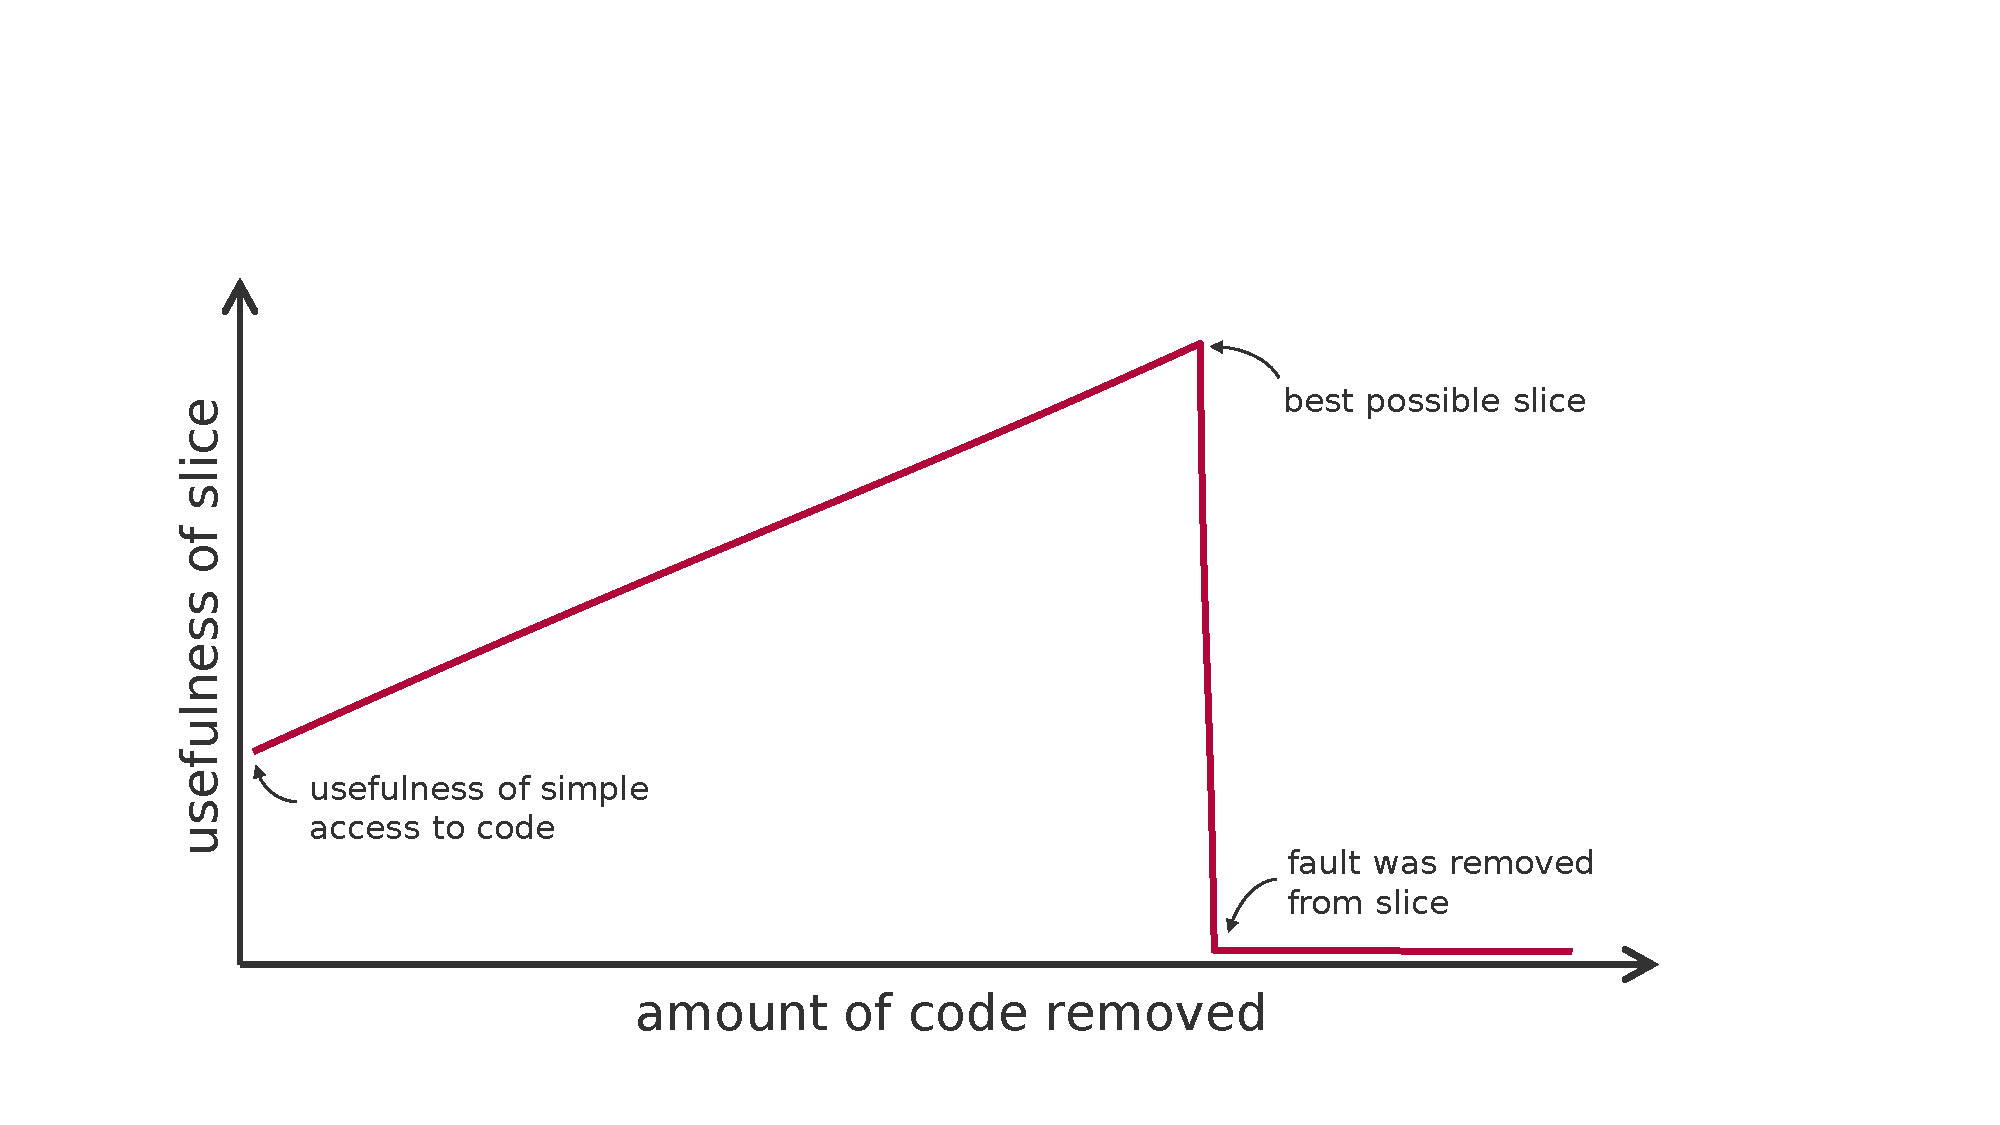
\includegraphics[width=.75\linewidth]{img/slice_usefulness}
\caption{As a slice becomes smaller its usefulness increases, until the fault itself is removed.}
\label{fig:slice_usefulness}
\end{figure*}

Subsequent work focused on increasing the precision of accurate slices, for example in the presence of pointers~\cite{atkinson02:program_slicing_using_dynamic, agrawal91:dynamic_slicing_in}.
In 2003, Zhang \etal\ presented three algorithms to efficiently compute "precise slices", i.e., slices that are "accurate" but contain little to no statements that could be removed~\cite{zhang03:precise_dynamic_slicing_algorithms}.
Like many other authors, Zhang \etal\ argued that producing small slices is essential if slicing is to be "an attractive option" for developers.
However, Korel argued that slicing too aggressively can also be dangerous, as
for program debugging the challenge is not necessarily to minimize the size of the slice at any cost but rather to minimize the size of the slice without the elimination of faulty program statements~\cite{korel98:dynamic_program_slicing_methods}.
\Cref{fig:slice_usefulness} illustrates the problem as a graph.
A slice that contains all the code is just as useful as having access to the code itself.
When more and more code is removed, the usefulness grows as less code has to be investigated by developers.
But when slicing becomes so aggressive that the code developers are actually looking for is removed, too, 
the slice's usefulness drops drastically.
Slicing algorithms therefore try to err on the safe side and are generally cautious when estimating whether code can be removed.

Between executable and "accurate" slicing algorithms, the former are the more conservative.
Their difference can be demonstrated with a small example.
In the code shown in \cref{lst:sliceAccurate}, line 9 is only executed during the second iteration of the loop.
Therefore, when choosing ´ratio´ in line 9 as a slicing criterion, "accurate" slicing algorithms can remove the assignment of the first array item in line 3.
This will reduce the size of the slice, as the call to ´complexComputation1´ is removed, but when the remaining code is executed, a division by zero will occur during the first iteration in line 7.
Korel argued that the correctness of a slicing algorithm can not be objectively determined if it is allowed to produce slices where the program fails~\cite{korel98:dynamic_program_slicing_methods}.
Without proven correctness, one risks falling off \cref{fig:slice_usefulness}'s usefulness cliff.

\begin{lstlisting}[float,caption={Code example for accurate slices.},stepnumber=2,numberfirstline=false,label=lst:sliceAccurate,language=Java]
	void main() {
			float[] data = new float[2];
			data[0] = complexComputation1(); // returns 0.5
			data[1] = complexComputation2(); // returns 5
			for (float f: data) {
					f = adjustValue(f);
					float ratio = 2 / f;
					if (ratio < 1) {
							System.out.println(ratio); // expected 0.2, got 0.4
					}
			}
	}

	float adjustValue(float value) {
			if (false && moreConditions()) { // bug in this line
					return value * 2;
			}
			return value;
	}
\end{lstlisting}

However, algorithms for both executable and "accurate" slices are allowed to remove the call to ´adjustValue´ in line 6 and can therefore hide the actual bug.
In general, bugs caused by wrongly skipped or missing code are difficult to locate with slicing.
Wang \etal\ addressed this problem by developing an algorithm to find "relevant" slices, slices including code that could have changed the state trajectory but was not executed~\cite{wang08:dynamic_slicing_on_java}.
Likewise, Ko \etal\ developed Whyline, a slicing-based tool allowing developers to ask "Why?" and, more importantly, "Why not?" questions~\cite{ko08:debugging_reinvented_asking}.

The usefulness of a slice depends not only on which code remains included, but also on what the developer wants to achieve.
While a slice may be suitable for solving one problem, for another problem the necessary code might have been removed.
By considering developers with a debugging problem as end users of a slicing tool, we can carry the trend of carefully reducing slice sizes to its logical conclusion: we define a "most useful slice" as exactly the subset of statements of a program that developers need to see in order to answer the question they are currently investigating.
Such a slice is not necessarily executable, "accurate", "precise", or "relevant", according to the established definitions, but rather captures the optimal combination of these conflicting properties.

Some approaches attempt to provide better slices by making assumptions about developers' information needs~\cite{sridharan07:thin_slicing}.
\todo{end this section here}
We argue that additional user input is necessary to provide better slices without risking to remove to much code.
Thus, to compute a "most useful" slice, we would have to add the developers' research question and current state of mind to a slicing algorithm's input.
This leaves us with two problems.
Firstly, we need to find a method to formalize a developer's entire state of mind, and secondly, we need to a way for developers to specify this data easily and correctly.
%While it may not be possible to achieve perfect "most useful" slices in one attempt, we can look into ways to approximate


%Alas, we cannot present a solution for either of these problems.
%\todo{
%However, as a step towards the goal of "most useful" slices, we developed a slicing algorithm that allows developers to easily get arbitrarily close to the smallest slice they need.}

\section{Additional Challenges in Enterprise Applications}
\label{sec:enterprise_applications}

\tmpStart
To better understand the development of modern business software, we interviewed five software developers from SAP, a German software corporation developing enterprise software to manage business operations.
From these developers, we gained insights on the development of four different projects:
\begin{enumerate}
	\item A software for liquidity risk management that analyzes the cash-flow of financial institutes to assess their liquidity,
	\item A customer analytics software to understand customer behavior based on collected data, which allows, for example, to identify particularly profitable customers or customers that plan to leave the company (e.g., clients of a bank who cancel all their standing orders),
	\item A product for predictive analytics that allows to estimate the probabilities for certain customer behaviors, such as switching distributors or suppliers. The analyses' results are integrated in a customer relationship management (CRM) system and recommend opportunities for salespeople, and
	\item The point-of-sales (POS) explorer, a dashboard that computes various key performance indicators (KPIs) on the revenue and profits of products based on retail data.
\end{enumerate}
%
All applications are designed to work on real-time data generated by respective transactional systems and were developed with an industry partner who provided requirements.

\subsection{Changing Characteristics in 3-tier Applications}

The design of all applications was based on the 3-tier architecture pattern, which divides an application into three layers~\cite{eckerson95:three_tier_clientserver_architecture}.
The \emph{presentation tier} displays information and receives input from the user,
the \emph{application tier} contains the application's business logic, and
the \emph{data tier} encapsulates data access and persistence.
The presentation tier is the application's front-end and runs on the client, while the application and data tier constitute the back-end and run on the server.

In traditional 3-tier applications, most of the code is implemented in the application layer.
For example, templates allow the application server to render web pages that can be displayed by a browser on the client.
When a dedicated client application is needed, keeping it small and simple reduces the overhead of maintaining and updating a large number of installations.
Either way, the client is little more than a terminal.

On the data side, object-relational mappers (ORMs) allow developers to implement data processing logic directly in the application.
This makes applications independent from specific database products and avoids introducing additional programming languages into the project.
Because application servers can be scaled more easily than databases, this also reduces the database bottleneck that can occur in applications with many users.

Many application frameworks, such as J2EE and Ruby on Rails, follow this philosophy and many tools have been developed to support development and maintenance in such ecosystems.
However, as we found in our interviews, the usefulness of many of such tools is decreasing as technologies and requirements change in the development of modern business applications.
For illustration, \cref{fig:3tier-changes} compares the architectures of exemplary classical and modern 3-tier applications.

\begin{figure*}[t]
\centering
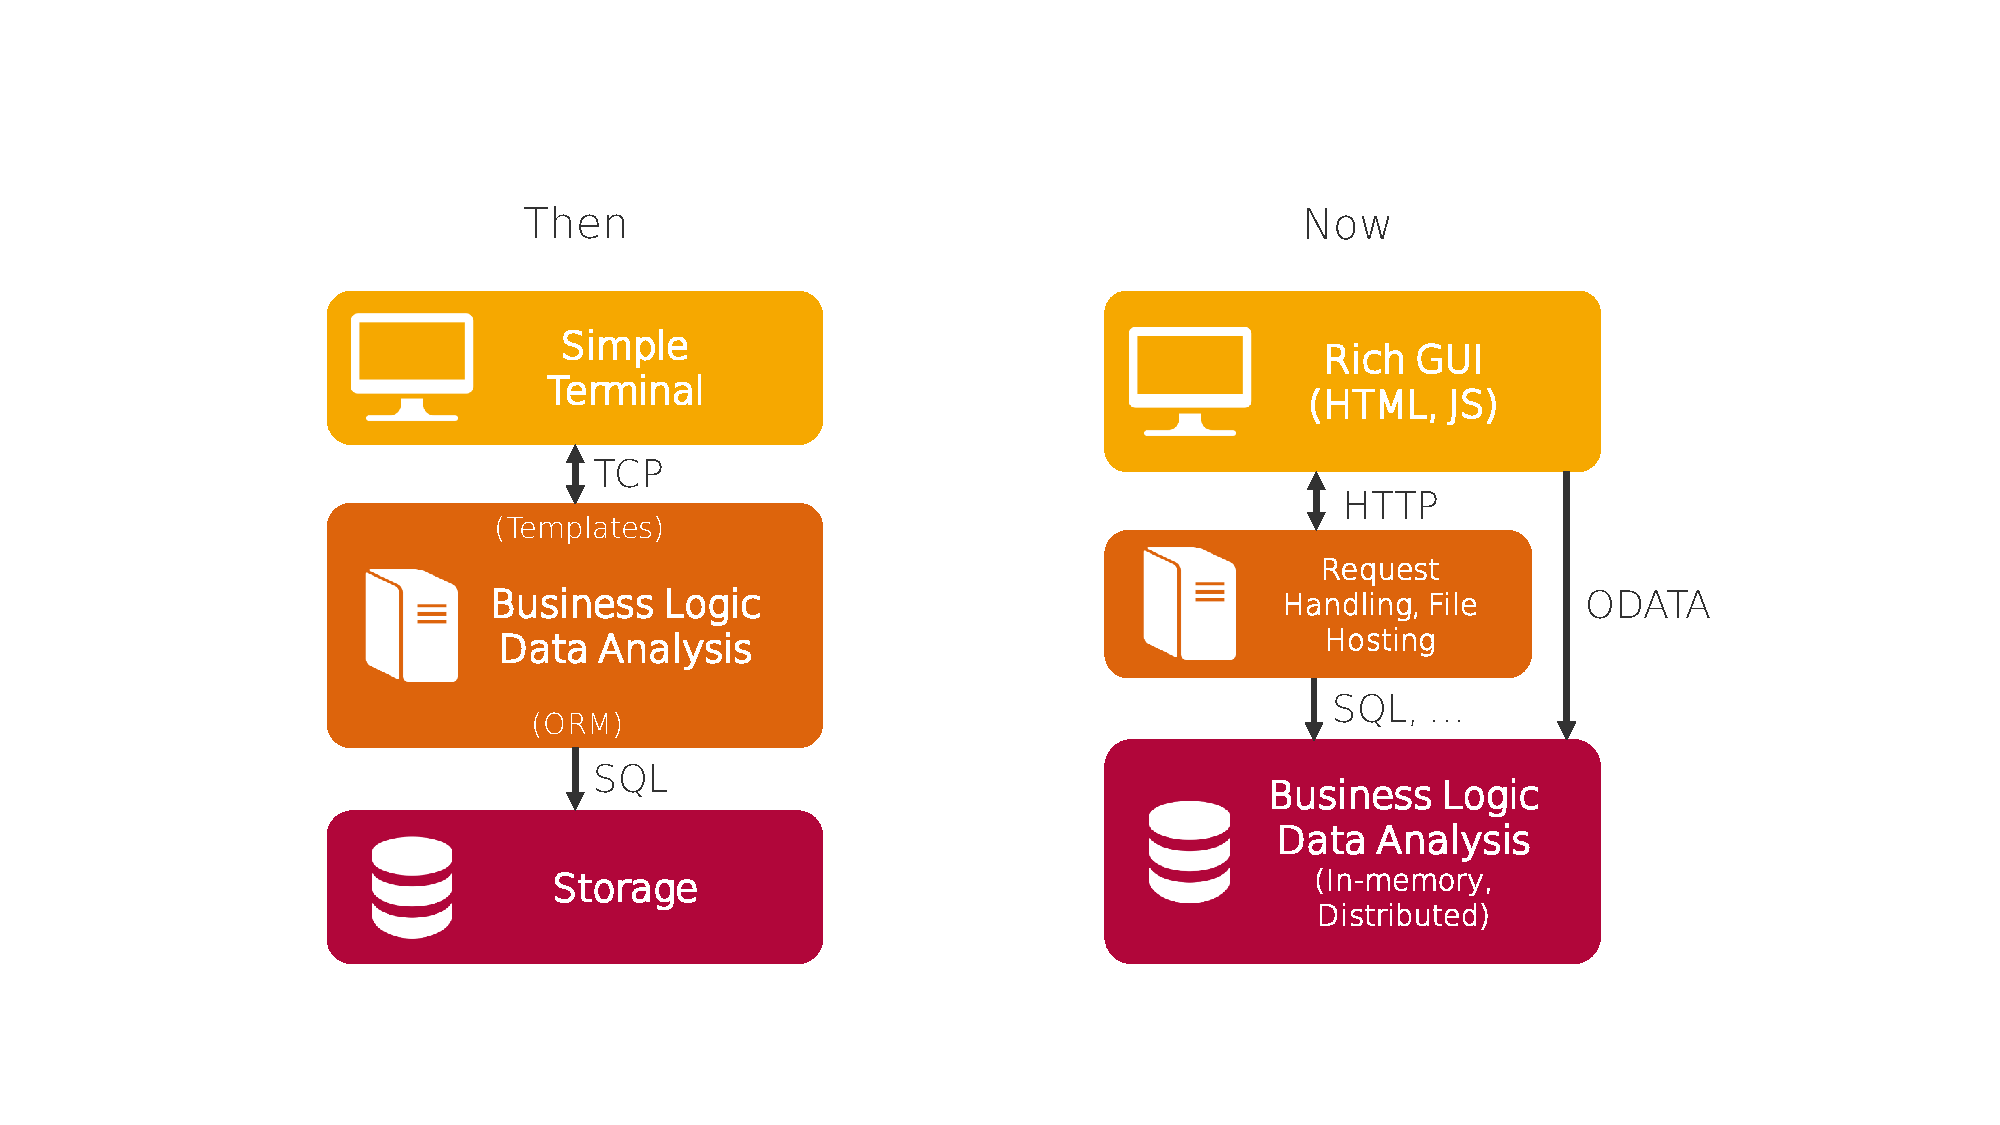
\includegraphics[width=.9\linewidth]{img/3tier-changes}
\caption{As a slice becomes smaller its usefulness increases, until the fault itself is removed.}
\label{fig:3tier-changes}
\end{figure*}

HTML 5 and JavaScript allow developers to build responsive and dynamic interfaces, which are increasingly expected by users.
Via HTTP and fast connections, megabytes of client code can be updated with every request so there is no longer a need to keep the client code minimal.
JavaScript-based GUI libraries eliminate the need for server-side templates as the entire GUI can be built in the client and data is dynamically loaded via AJAX requests.

With big-data becoming more important for many companies, it is no longer feasible to handle all data operations in the application layer.
Even transactional systems contain a large fraction of analytical operations~\cite{krueger10:a_case_for_online} and high-performance databases can handle such queries faster than application-level code~\cite{plattner09:a_common_database_approach}.
Even for transactional operations, the usefulness of ORMs is doubted as they can introduce other organizational and architectural problems~\cite{neward06:the_vietnam_of_computer}.

All developers reported that their projects followed these new architecture patterns.
To achieve sufficiently low response times, data is stored in \emph{SAP HANA}, a high-performance in-memory relational database.
The application layers run in \emph{SAP HANA Extended Application Services}, an application and web server environment on top of the database.
In each project, the front-end is implement in \emph{SAPUI5}, a JavaScript GUI library based on jQuery.

For the fourth project, the POS explorer, we were given full access to the code base.
At the time of the interview, the whole application had 11 thousand lines of code, libraries excluded.
55\% of the code (i.e., about 6000 lines) was client-side JavaScript, of which about 12\% (725 lines) was data querying code.
The application layer consisted of 2000 lines (18\%) of server-side JavaScript (similar to node.js), while the database layer contained 3000 lines (27\%) of stored procedure code.
Data schema definitions are not included in the line counts, as the data is defined and provided by other applications.
% client/js					2397
% client/fragment		3750
% client/view				 133
% client -- query		 600 // client 6280 -- 6000
% app/xsjs*					2250 //  -- 2000
% db/procedure			2991 // -- 3000
% // 11521

Standards like \emph{OData}~\cite{chappell11:introducing_odata} allow clients to submit arbitrary queries to the database, entirely eliminating the need for a middle layer.
It should be noted that this setup is different from the classical 2-tier architecture, where a trusted client has full access to the database.
OData still maintains security concerns such as authentication, authorization, and visibility of data, which was previously a responsibility of the application tier.

For one of the projects, the developer reported that they have no application layer code at all.
The application, he estimated, consisted of 90\% client-side JavaScript, of which one-third was OData client code, and 5\% OData service configuration which passed requests to stored procedures that constituted the remaining 5\% of the project.

In conclusion, due to increased complexity of interactions between the different layers it is no longer sufficient to be able to debug each layer on its own.
Instead, tools are needed that help developers to debug and understand the application as a whole.

\subsection{Debugging 3-tier Business Applications}

All developers reported that changes in software development processes affected the way how bugs are handled.
In the past, large applications had separate development teams for front-end, business logic, and data management.
If a team found that a bug was not caused in their respective domain, the responsibility was passed on to the next team.

Agile development methodologies, such as Scrum or Extreme Programming, discourage dividing teams by technology layer.
Instead, requirements and, if necessary, sub-teams are now grouped around feature sets.
Thus, while there still may be developers who are specialized on one of the application tiers, every developer is expected to be able to work on and to debug every layer.
This increases the need for making debugging tools for each layer easily available to all developers.

The existence of bugs is typically discovered by observing unexpected data in the user interface.
Then, developers use their browser's development tools to examine the request with which the data was obtained.
In most cases, the response data is passed unchanged to the GUI components and the incorrect data can be tracked directly back to the response.
Here, the first uncertainties occur as it is often not obvious whether the request was submitted with incorrect arguments or whether the error is on the server-side.

If developers decide to continue to the application code, they determine which server function is called, connect a debugger to the application server, set a breakpoint, and re-submit the failing request.
Then they use the debugger to understand how the request is processed.

If no fault can be found, they now need to determine if the results returned by database queries are correct.
For queries that include complex views or stored procedures, this is not an easy task.
Furthermore, if the query was composed at runtime, developers also need to determine the actual query string and which arguments were used.
After that, they can use the tools provided by the database client to analyze the query and verify the result.

Using these methods, developers move up and down the stack until they find the root cause of the bug.
Generally, all developers reported that they preferred to work with a top-down approach, i.e., they try to first understand the interaction between the layers before starting a debugger to narrow down possible locations for the bug as early as possible.
However, while the developer tools of browsers were reported to be somewhat useful for this task, no such tools exist to understand the interaction between application and data tier at a glance.

Overall, frequent switches between tools were reported to be a major distraction when trying to focus on the program flow.
Often, multiple monitors were used to allow developers to access all tools more quickly, but all developers wished for better integration between tools.
\tmpEnd

%\section{Requirements for an Enterprise Application Debugger}
%\label{sec:requirements}
%
%Based on what we learned about
%
%
%Requirements
%- Iterative approach
%- Identify related statements \cite{ko07:information_needs_in_collocated}
%- support short-term memory \cite{fry97:programming_on_an_already}
%- reduce problem size



%Finding bugs in complex code is a demanding task for developers and many tools and techniques have been developed to support this process.
%However, complex system architectures add another level of difficulty to fault localization.
%
%Server-based applications typically use a three-tier architecture.
%The database layer is used to persist the application's domain model.
%The user interface layer shows application data to the user and accepts user input.
%In between, the application layer contains most of the business logic which defines the application's workflows, how to handle user requests, and how to collect and present requested data.
%
%When most code resides in the application layer, so do most bugs and the well-known debugging tools can be used to locate them.
%However, in more recent years, the classic three-tier architecture changed in multiple ways.\todo{source}
%
%\subsection{Database Layer}
%
%The amounts of data to be handled by server-based applications are always increasing.
%Recently, big data has become a very important topic for many enterprises.
%To guarantee optimal performance on large data sets, more and more data handling code has to move closer to data, into the database layer.\todo{source}
%
%tbd: describe UI technologies
%
%\subsection{User-Interface Layer}
%
%Better web browsers, HTML 5, and Java Script replaced the terminal application.
%It is now easier to manage client code as updates are automatically requested via HTTP.
%This way, more business logic could move into the UI layer to provide a better user experience.\todo{source}
%
%tbd: describe UI technologies
%
%\subsection{Application Layer}
%
%Remaining AppLayer: request mapping, security
%
%Java, Rails, Node.js
%
%skip applayer with ODATA and user-management in database
%
%\subsection{Debugging the Stack}
%
%Both modern browsers and databases have debugging capabilities that are useful to locate bugs within their respective layers.
%Alas, not every bug can be tracked down to a single code location. 
%Sometimes, it is a combination of mismatching assumptions in different code locations that compose the fault \todo{source}.
%In a complex system, these locations need not reside in a single component, but can be scattered across all layers.
%Likewise, the infection chain that connects the observed failure with the fault in the code can cross several system boundaries.
%
%In both cases, no single debugging tool is sufficient to locate the bug, as each debugger can only be used to debug its respective system.
%The resulting tool and context switches impose a mental overhead that distracts developers from the actual problem.
%
%The problem is further amplified with service-oriented architecture (SOA), and micro-services in particular.
%To achieve better scalability and faster life-cycle management, applications are broken down into many independent systems, each with their own database.
%While the resulting modularization can help to limit the consequences of software failures to smaller sub-systems, the difficulty of locating cross-system bugs increases further.
%
%%The debugger is one of the most important tools of a software developer. 
%%It allows to observe and inspect a program’s execution and can be used for many purposes, such as bug detection and code comprehension. 
%%Workflow
%%\\- failure observed
%%\\- error in state- > find the code
%%\\- either GIGO, then repeat, or...
%%\\- fault in code


\chapter{Interactive Dynamic Slicing}

\tmp{
% Context: debugging and slicing
In many cases, software bugs don't cause the software to fail, i.e., to deviate from expected behavior, immediately.
To actually find the bug, developers have to follow the chain of erroneous state from the observed failure backwards to the bug~\cite{zeller_why_2009}.
Many approaches exist to support this process~\cite{wong_survey_2016}.

Debuggers allow to inspect the state of a running program and to understand its impact on the program's behavior.
Back-in-time, or "omniscient" debuggers (ODBs) even make it possible to follow the infection chain backwards through time, removing the overhead of frequently restarting the debug session~\cite{lewis_debugging_2003}.
However, developers still need to manually identify the relation between states without spending too much time in irrelevant parts of code.
This often requires a high familiarity with the code, which is not always given.
%
%when programmer needs better understanding, turns to debugger\\
%as knowledge grows, question change\\
%linear nature of debugger, repetitive task of restarting\\
%omniscient debugging improves productivity by reducing mental overhead\\

Weiser has shown that programmers think not only in modules, but in related statements~\cite{weiser_programmers_1982}.
Slicing is a technique to produce subsets of a program relevant to a given criterion.
Dynamic slicing also considers the program input, which allows to remove even more irrelevant instructions~\cite{agrawal_dynamic_1990}.

% Problem: tool integration
Slicing suffers from a similar problem as debugging:
every time the developer's question changes the slice has to be recomputed, which can interrupt the developer's flow even if it only takes a few seconds.
Furthermore, every time developers need to switch between slicer and debugger, another interruption occurs.
Slicing is rarely used in practice~\cite{perscheid_studying_2017} and the separation of tools might be part of the problem.

% Significance
It has been shown that slicing can be useful to improve developer productivity~\cite{weiser_programmers_1982, agrawal_dynamic_1990}, especially for developers dealing with very complex or unfamiliar code.

We present a new approach that combines omniscient debugging and dynamic slicing.
While developers omnisciently debug a dynamic slice, at any point they can add or adjust the slicing criteria and changes are applied instantly, without interrupting the debug session.
A new UI component, the Slice Navigator, provides a unique view on the execution by combining relevant information from both the ODB and the slicing subsystem.

The contributions of this paper are threefold:
\begin{itemize}
	\item A new dynamic slicing algorithm allows quick and iterative refinement of the slicing criteria to adapt the slice to changing developer questions.
		Based on previous work, developers can formulate their question by choosing from different dependency types that will change the outcome of the slice~\cite{treffer_dynamic_2014}.
	\item The \emph{Slice Navigator} is a UI component that bundles access to the debugger and the slicer.
		It provides context for the current instruction by showing relevant parts of the slice, allows developers to iteratively refine the slicing criteria, and serves as an alternative to breakpoints and stepping.
	\item The integration of dynamic analyses directly in the debugger not only reduces interruptions in developer flow by minimizing context switches between tools and shortens waiting time as recorded run-time data can be re-used; it also allows for a new debugging workflow where developers can isolate a bug by iteratively slicing away correct code.
\end{itemize}
}

\section{A New Debugging Workflow}

\section{Incremental Configurable Slicing Algorithm}

\section{Evaluation}


\chapter{Bringing Omniscient Debugging Down to the Database}
\label{sec:db_odb}

\newcommand{\tool}{TAR\-DISP}
\newcommand{\SQLextension}{Back-in-time SQL}
%%Context: Debugging and Back-in-Time
%Finding defects in code is a frequent task for every programmer and is often difficult even with a deep understanding of the system.
%To localize failure causes, they examine involved program entities and distinguish relevant from irrelevant behavior and clean from infected state. 
%However, common symbolic debuggers do not support identification of such infection chains very well because they only provide access to the last point of execution without access to the program history.
%Back-in-time also known as omniscient debuggers simplify the debugging process by making it easier to follow cause-effect chains from the observable failure back to the causing defect~\cite{lewis03:debugging_backwards_in_time}.
%These tools provide full access to past events so that developers can directly experiment with the entire infection chain. 

As we have seen, specialized debugging tools can significantly reduce the time needed to locate a bug.
Consequently, many tools and methods that improve debugging have been developed in the past decades~\cite{wong16:a_survey_on_software}.
However, few of these debugging tools consider an important component of every enterprise application: the database.
Back-in-time debuggers, for example, exist for many object-oriented programming languages, such as Java, C++, or JavaScript~\cite{feldman88:igor_a_system,lewis03:debugging_backwards_in_time,barr16:time-travel_debugging_for_javascriptnode,wong16:a_survey_on_software}.
These languages are typically used in the front-end or application layer of a multi-tier application.

%SQLScript\footnote{SQLScript is a proprietary SQL extension for stored procedures in SAP HANA~\cite{sap16:sap_hana_sqlscript_reference}.}. %hofer_design_2006


The application layer of a multi-tier application can interact with the database in multiple ways.
For object-oriented programming languages, \acp{orm} can abstract from database-specific logic by automatically generating queries and converting all data from and to native objects.
In this scenario, the database is mostly used as a persistent storage of business objects from the application layer.
As already discussed in \cref{sec:enterprise_applications}, "\nameref{sec:enterprise_applications}", 
this is not sufficient for modern applications that handle large amounts of data.

%a database connectors like ODBC or JDBC and 
By using query languages like SQL, the application layer can submit arbitrary queries to the database to store, manipulate or obtain data.
Data-heavy operations can be executed faster by sending them to the database~\cite{plattner15:the_in-memory_revolution_how}, even while the data handling logic remains in the application layer
By using language extensions such as SQL/OLB~\cite{eisenberg98:sqlj_part_0_now}, it is even possible to include database queries as native language elements.

However, not all operations can be expressed in a single query.
When queries are submitted from the application layer, intermediate results have to be passed between application layer and database multiple times.
In big-data applications, where the communication channel between database and application is a strong bottleneck, this pattern must be avoided~\cite{plattner15:the_in-memory_revolution_how}.
Hence, the third approach of handling data-heavy operations is to implement them as stand-alone scripts, also called stored procedures, that, when called from the application, run directly in the database.
This reduces communication overhead between layers and allows the database to apply further optimization, such as reordering queries or choosing when to materialize intermediate results.

Basic debugging support exists for many of these methods and supports forward-in-time debugging and inspecting query results while the program is stopped.
However, there are, to the best of our knowledge, no omniscient debuggers that include the database and support SQL queries or database scripts.

%Database languages like SQLScript, a proprietary language for stored procedures in SAP HANA~\cite{sap16:sap_hana_sqlscript_reference}, 

\tmpStart
%Problem: Back-in-time debugger missing for database-level
This is mainly because of two reasons. 
First, back-in-time debuggers typically create a significant overhead on performance and memory consumption~\cite{lewis03:debugging_backwards_in_time,pothier07:scalable_omniscient_debugging,lienhard08:practical_object-oriented_back-in-time_debugging}.
It seems unfeasible to use a back-in-time debugger on top of a database script that processes billions of records.
Second, current back-in-time debugging concepts cannot handle side-effects outside their system that usually happen in writing operations during INSERT and UPDATE statements. 

%Significance: Especially, in business software much development is based on database scripts. 
Due to high performance requirements of handling big data in business applications, companies like SAP have not only a strong demand to move code closer to data~\cite{plattner15:the_in-memory_revolution_how} but also the need to improve development tools at the database-level. 
As existing tools mostly work on the application level, are limited to specific points in time, or work only on an abstract query plan, developers are often left alone when it comes to debug and understand the results of their queries and stored procedures.
We argue that a back-in-time debugger at the bottom of the technology stack is able to close this gap and can support developers in developing and maintaining their queries more efficiently. 
\tmpEnd

\tmpStart

%Solution
We bring the concept of back-in-time debugging to the database and developed \emph{\tool} as an implementation of our approach.

\begin{itemize}
	\item \emph{\tool} ("Tracing And Recorded Data In Stored Procedures") is a back-in-time debugger for stored procedures which can be installed in the SAP HANA in-memory database and programming platform.
		Using \tool, developers can move freely through the execution time of a stored procedure and inspect control flow, variables, and intermediate results.
	
	\item \emph{\SQLextension} is an extension to SQL allowing developers to submit arbitrary queries against previous states of the database 
		and to compare multiple points in time with one query.
		\tool\ provides a console for developers to submit \SQLextension\ queries which use variables or points in time from the current debug session.

	\item \emph{Very low overhead} when recording run-time data and the efficient querying of past database states allow developers to use \tool\ as the default tool for debugging database scripts even on large data sets.
	
\end{itemize}

We evaluated \tool\ with the help of SAP colleagues who worked on a project called \emph{Point of Sales Explorer}~\cite{plattner15:the_in-memory_revolution_how}, which makes heavy use of stored procedures. 
The interviews indicated that failures in stored procedures can be investigated more efficiently with \tool\ than with other existing database development tools.

\tmpEnd

%\subsubsection{Design Concept}
%pros and cons of post mortem,
%pros and cons of database
%discussion insert only
%final decision
%
%\subsubsection{Prototype: Architecture and Schema}
%figure: architecture
%data schema
%tracing code generation and examples
%
%\subsubsection{BiT SQL}
%
%\subsubsection{-TimeTravel queries}
%
%\subsubsection{-TimeDiff queries}
%
%\subsubsection{Evaluation}

\section{Back-in-Time Debugging in Stored Procedures}

In \cref{sec:omni-debugging}, "\nameref{sec:omni-debugging}", we discussed different approaches for implementing back-in-time capabilities in debuggers.
A snapshot-based debugger records program memory at certain intervals, additionally logging I/O-operations to make program re-execution deterministic when the program accesses external resources.
An omniscient debugger records a full execution trace.
This creates a larger overhead on memory and runtime, but allows the debugger to restore program state from any point in time in a post-mortem analysis.
Hybrid approaches record only the control-flow and partial memory snapshots, recovering the remaining state by re-executing parts of the program.
All approaches have in common that they simulate external resources from the program's perspective, but do not allow developers to inspect the resource itself.

From the debugger's perspective, the database is such an external resource and is therefore not covered by back-in-time features by default.
This is a problem for developers debugging database applications.
To evaluate the correctness of a piece of code, it is usually not enough to only see the result of queries in the program.
Instead, developers need to look into the data and maybe even run their own ad hoc queries to understand whether the program behaves correctly.

When including the database in the execution trace, a back-in-time debugger faces two additional problems:
First, much of the data processing happens outside of the program's scope.
Sometimes, state that has impact on a query's result remains entirely in the database and is practically invisible to the application debugger.
The only way to examine such state is through specific database queries.
Second, the debugger can not easily track changes in the state, because the impact of an insert, update, or delete statement is not reported back to the application in the necessary detail.
This affects determinism when re-executing earlier parts of the program.
With live debugging, sometimes this can be mitigated by resetting the database before restarting the program, but a post-mortem analysis can not easily examine intermediate database states when they have been changed.

In stored procedures, result variables are an additional challenge.
These variables represent the result of a query and can be used in subsequent database statements without havin been fetched into the program
In fact, the database may chose to not materialize intermediate results at all.

\tmpStart
Either way, this increases the amount of invisible state, sometimes only for a few instructions, other times for the entire length of the program.
Furthermore, as trace data usually exceeds program data by orders of magnitude, we expect that tracing the processing of every tuple in a large database is not feasible.

With \tool, we focused on stored procedures because they are executed close to the data and, thus, more efficient in handling large data sets.
This does not limit the general validity of our results, as a debugger for stored procedures faces all of the challenges described above.
\tmpEnd

\subsection{Replaying a Stored Procedure}

An application using a database to manage its state create several problems for debugging tools.
However, giving the debugger direct access to the database can open up new possibilities.

The most immediate advantage is that the database persists state beyond the program execution.
Even post-mortem, the state can be directly accessed by the debugger.
Especially in big-data applications, most operations do not change large parts of the state at once.
Depending on the problem scope and length of the debug session, most of the program state likely remains unchanged.
Knowing that the state will still be available, it can be excluded from the execution trace.

Furthermore, programs that rely on the database for data processing have on fundamental difference compared to other programs:
all instructions handling large data sets (i.e., SQL statements) are declarative.
Instead of providing a concrete algorithm for performing the operation, an SQL statement describe the outcome on an abstract, logical level.
At this level a statement can be analyzed without knowing how it is physically executed.
Even if the database later decides to execute a query using a different query plan, this has no impact for a developer trying to understand the functional correctness of a program.
Thus, there is no need to trace the internals of a query's execution like the processing of an array would have to be traced.
As long as the underlying data does not change, the query results need not be recorded either.
For some purposes it will be helpful to record some meta information, such as the execution time or the number of results, but even this data can be recovered later if needed.

Both advantages can only be exploited if the underlying data does not change.
However, given direct access to the database, the debugger can use it efficiently manage old state, too.
Data is already in a format optimized to be processed by the database and does not need to be transferred into another system this way.
With the ability to restore previous states of the database, 
\tmpStart
all that is needed to reproduce the execution of a stored procedure is a sequence of execution steps.
Each step represents an instruction that has side effects on the database or assigns a value or result set to a variable.
As there is, on the conceptual level, no concurrency in a stored procedure, we can use sequential numbering to track the order of steps.
If applicable, a step has a target name, such as the name of a variable or stored procedure, and a string representation of the value, which can be shown to the user in the debug view.
If the step involves a database statement, we also need a time stamp to be able to reproduce the query.
\tmpEnd

\begin{figure}
	\centering
		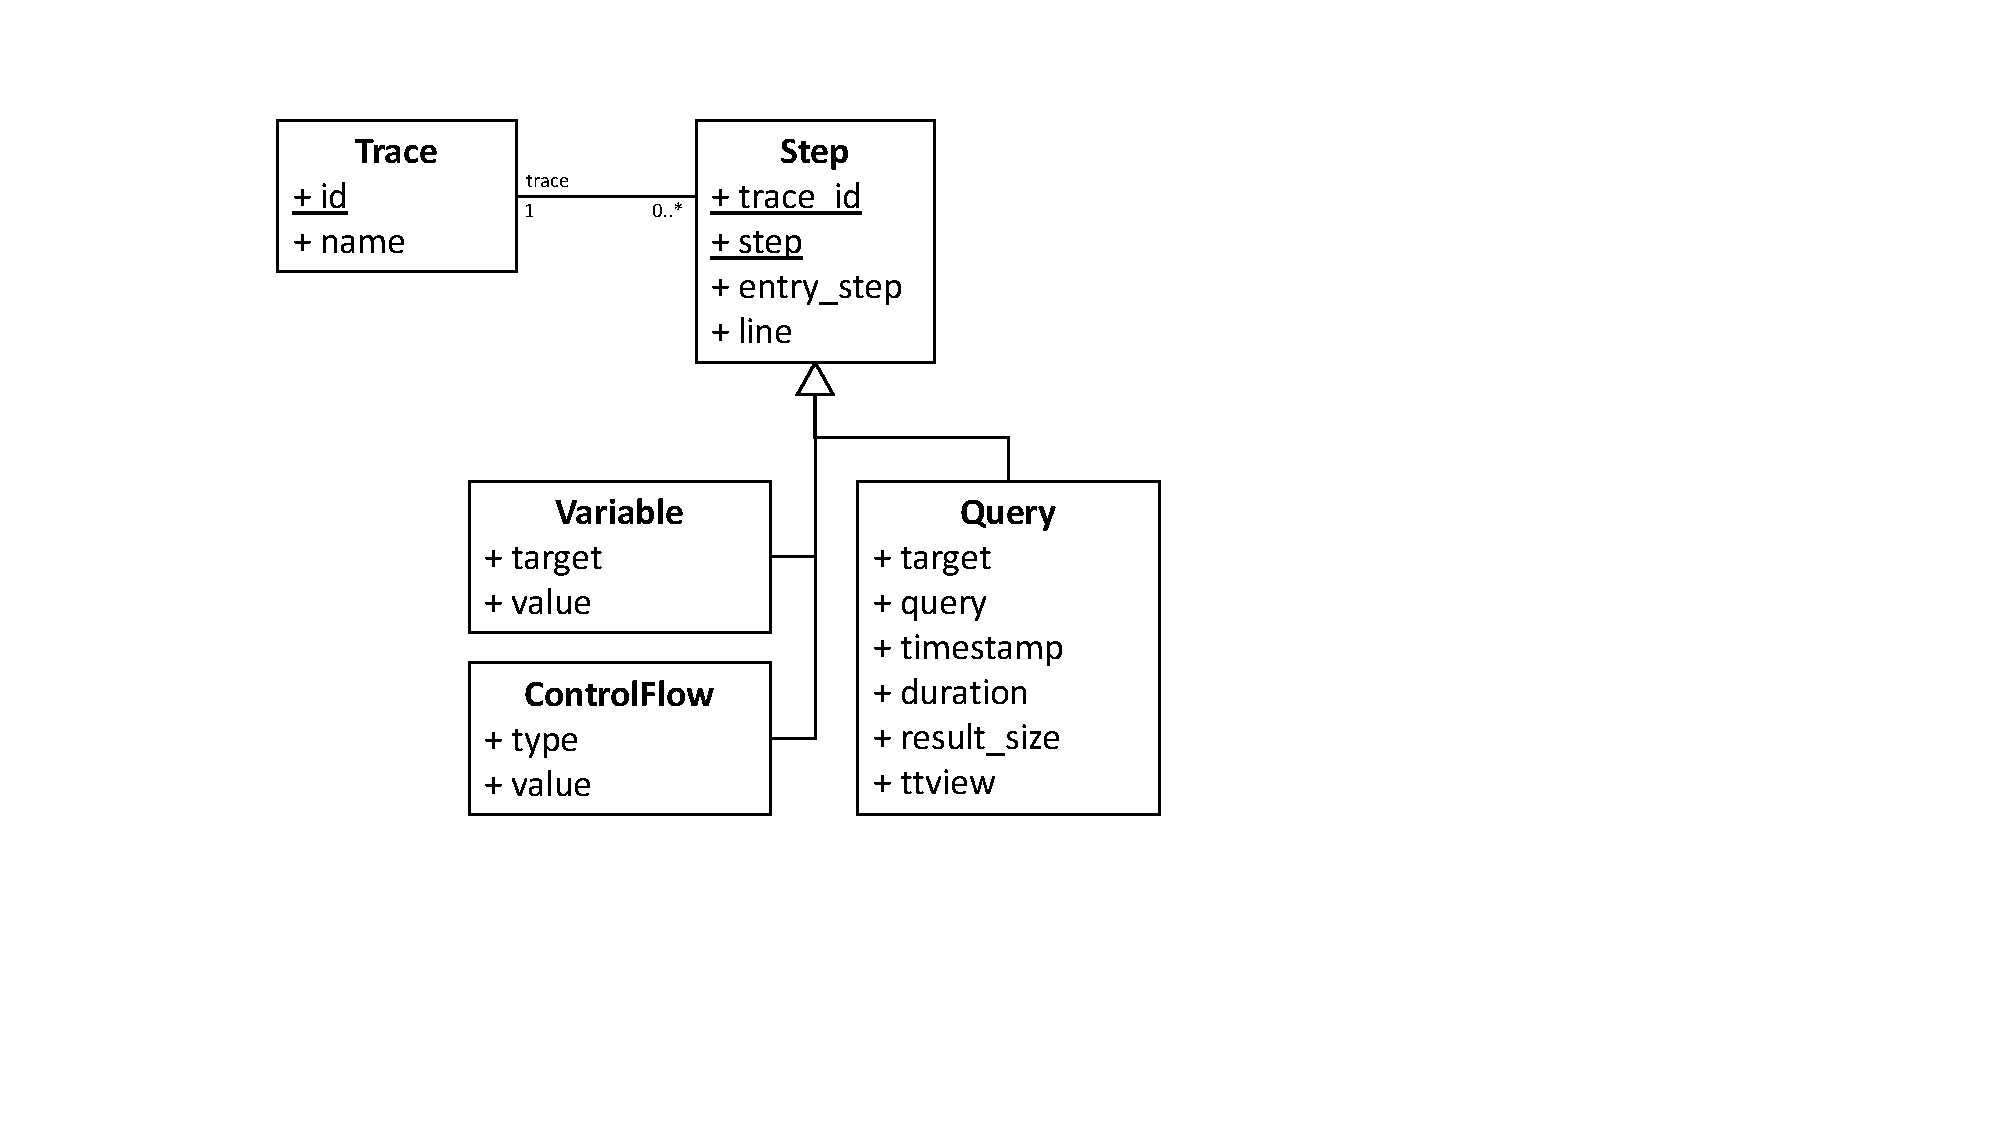
\includegraphics[width=0.9\linewidth]{img/model_sqlodb}
	\caption{Data model of the Stored Procedure debugger.}
	\label{fig:model_odb}
\end{figure}

\Cref{fig:model_odb} shows the relational data model we use to store the required information.
On top of the minimal required data, we record some additional information to simplify interpreting the trace later on.

Along with each query invocation, its atomic arguments are recorded.
Even though these values can already be derived from the execution trace, storing them explicitly simplifies the process of restoring query results by removing the need to analyze code outside the query itself.
Furthermore, we record the execution time and the number of rows in the result set for each query.
This information, too, is not strictly needed and can be recovered by re-executing the query.
However, we found that directly providing this information can be helpful to developers, especially for long-running queries.
Lastly, we record the name of a view than can be used to later reproduce the query result.
The view is specifically generated by the debugger, as will be explained in the next subsection.

Because the runtime model of SQLScript is much simpler than that of Java and it was not our goal to create a fully featured debugger for the imperative part of the language, the data model of this debugger is much simpler than that of the Java back-in-time debugger~(\cf \cref{fig:model}, \cpageref{fig:model}), respectively.
This does not limit the general validity of our approach.
The database query as an extra event type could also be added to the Java debugger's trace model and the debugger would handle these queries in just the same way.

\subsection{Reproducing Query Results}

\tmpStart
With the recorded trace data, the debugger has enough information available to replay the execution and to re-execute any query.
However, the query will only yield the same results as long as the underlying data has not changed.

In general, one can expect that debugging will take place on a development machine where no other data manipulation occurs, 
but in cases where this assumption doesn't hold the debugger might end up showing wrong or misleading data the developer.
Furthermore, the debugged stored procedure itself may change the data, which will cause a query to return different results at different points in time.
\tmpEnd

Thus, to fully support back-in-time debugging on a database, the debugger needs to support querying previous database states.
Minimally, it should be possible to re-submit queries from the program against the database states at which they were originally run.
In this case, it would not be necessary to manage intermediary states when multiple updates occur in a row, and only tables actually used by a query would need to be reverted.

However, we believe it would be very helpful to allow developers to submit arbitrary ad-hoc queries against any previous database state.
In a relational database schema, tables often contain ids that reference entries in other tables.
To understand the outcome of a query, a developer might need to access such tables even when the program did not.
In other cases, developers want to run entirely different queries to find specific records or verify certain properties of the data.
We considered four different strategies for managing and querying old database state.

%\paragraph{\emph{Application-level Logging}}
\subsubsection*{\emph{Application-level Logging}}

In many business applications, data is never deleted, at least in the short term.
Legal reasons or business cases may require that all changes to an entity are tracked with time stamps.
When the ability to restore old entries is already a requirement of the software, the debugger can re-use these mechanisms when replaying a stored procedure.

\renewcommand{\baselinestretch}{1.0}
\begin{table}
	\centering
	\begin{tabulary}{\textwidth}{rcrp{2cm}>{\centering}p{1.8cm}>{\centering}p{1.8cm}J}
	\toprule
	\multicolumn{7}{c}{\lstinline[language=HanaSQL]+SELECT * FROM products WHERE id = 17+} \\%[4pt]
	\cmidrule(lr){1-7}%\midrule
	id &	name	& price & description & created\_on & valid\_until & change\_reason \\ \midrule
	17 &	Pen &	0.99	& Pen with \newline balck ink & 2018-06-01\newline 08:00:00 & 2018-06-01\newline 09:00:00 & Initial version \\[22pt]		
	17 &	Pen &	0.99	& Pen with \newline black ink & 2018-06-01\newline 09:00:00 & 2018-06-15\newline 08:00:00 & Typo in description \\[22pt]	
	17 &	Pen &	1.99	& Pen with \newline black ink & 2018-06-15\newline 08:00:00 & \emph{null} & Price changed \\		 \bottomrule
	\end{tabulary}
	\caption{An excerpt of a table containing product data, showing revisions of a single entity}
	\label{tab:applogdata}
\end{table}
\renewcommand{\baselinestretch}{\defaultbaselinestretch}

\Cref{tab:applogdata} shows multiple revisions of an entity in a table of product data. 
When only the most recent revision is needed, which will probably be the case for many operations, developers have to explicitly add a filter condition to select the correct tuple.
For instance, the following query selects the most recent version of the entity shown in \cref{tab:applogdata}:
\begin{lstlisting}[language=HanaSQL,frame={},numbers=none]
  SELECT * FROM products WHERE id = 17 AND valid_until IS NULL
\end{lstlisting}
When developers submit this query in the context of a back-in-time debug session the debugger has to rewrite the query to select the entity valid at the respective point in time:
\begin{lstlisting}[language=HanaSQL,frame={},numbers=none]
  SELECT * FROM products WHERE id = 17 
	  AND created_on < :dbgtime 
	  AND (valid_until >= :dbgtime OR valid_until IS NULL)
\end{lstlisting}
To simplify the process of query rewriting, especially when the validity columns ("created\_on" and "valid\_until") are used in more complex conditions, the debugger can generate back-in-time views that provide previous versions of the table.
\Cref{lst:bitview} shows the declaration for a back-in-time view in SAP HANA.
By using this view, instead of rewriting the where clause, the debugger only has to replace the table reference:
\begin{lstlisting}[language=HanaSQL,frame={},numbers=none]
  SELECT * FROM _BIT_products(:dbgtime) WHERE id = 17 AND valid_until IS NULL
\end{lstlisting}

\begin{lstlisting}[language=HanaSQL,float,caption={Definition statement for a parameterized view, showing a previous version of table "products", in SAP HANA's SQL dialect},label=lst:bitview,firstnumber=1,stepnumber=5]
	CREATE FUNCTION _BIT_products(IN dbgtime TIMESTAMP)
	RETURNS TABLE 
	LANGUAGE SQLSCRIPT AS
	BEGIN
		RETURN 
		  SELECT id, name, price, created_on, change_reason,
						 (CASE WHEN valid_until < :dbgtime 
							THEN valid_until ELSE NULL) AS valid_until
			FROM products 
			WHERE created_on < :dbgtime
	END;
\end{lstlisting}

%float,caption={Query to select the most recent tuple},label=lst:selectrecent

The main advantage of using application-level logging for debugging is that no additional memory and no specialized logging is required.
The latter implies that this approach can be easily transferred to databases of different vendors, as only the SQL dialect for creating and calling back-in-time views needs to be changed.

However, to use this approach the debugger needs to know exactly how logging is implemented, \ie a part of the debugging system must be specifically configured to work with the application's data schema.
Furthermore, the debugger operates under the assumption that the application does not introduce errors in the log data.
As a result, bugs that affect the log are especially hard to debug.

In some cases, application-level logging may only be available for some of the tables.
Luckily, this approach can be mixed with other strategies to manage old state.

\subsubsection*{\emph{Debug-level Logging}}

When the database schema does not support retaining old entities, the debugger can introduce additional tables to store such data.
Then, as with application-level logging, the debugger generates views that combine the current and history data and rewrites back-in-time queries accordingly.

To avoid copying entire tables, however, the debugger needs to know which tuples are affected by insert, update, or delete statements.
While it is possible to obtain this information by running appropriate queries before and after the change, we expect the overhead and additional complexity to render this approach impractical.
Instead, we looked at ways of using existing database features to implement logging more efficiently

\subsubsection*{\emph{ACID Transactions}}

Transaction are a database feature that allow multiple queries to be combined into one logical operation.
While many users concurrently access the database, transactions enable reliable operation and valid data when they satisfy the ACID properties: atomicity, consistency, isolation, and durability.

For debugging purposes, the isolation property can be used to support back-in-time functionality.
By running data manipulation statements in a transaction, it is still possible to query the database from before the transaction started as long as it is not committed.
Using nested transactions, as shown in \cref{fig:bit_transactions}, allows developers to query intermediate points in time.

\begin{figure}[t]
\centering
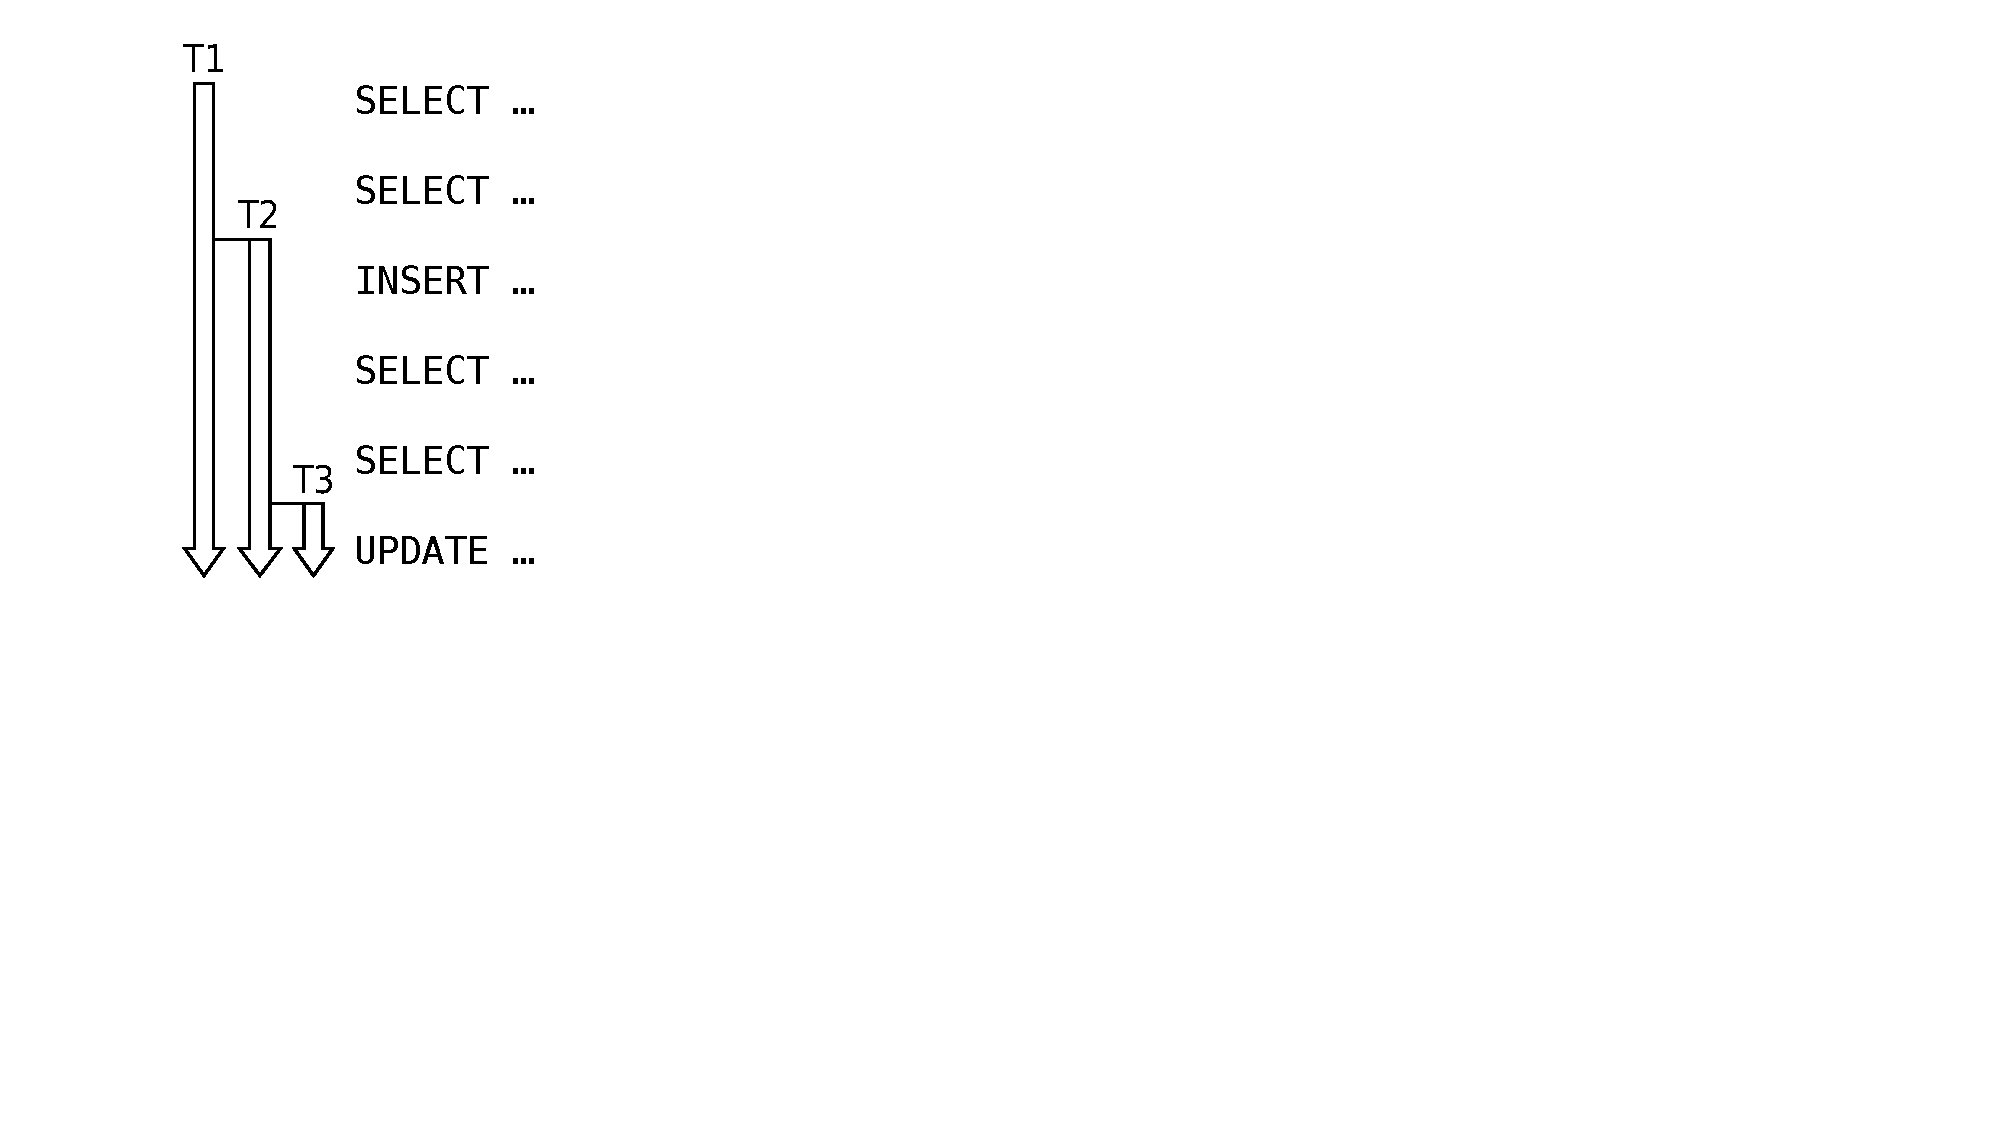
\includegraphics[width=0.3\linewidth]{img/bit_transactions}
\caption{Nested transactions allow reversing data manipulation queries.}
\label{fig:bit_transactions}
\end{figure}

An additional advantage of running a debug session in a transaction is that developers can manually modify the data to explore how the program would behave under different conditions, without threatening data integrity.
However, the success of applying transactions for back-in-time debugging depends on how transactions are implemented in the database.
Transactions are not intended to be left uncommitted for several minutes and developers might accidentally lock important tables from access for others or find their debug session suddenly canceled by the database.

\subsubsection*{\emph{Insert-only Databases}}

\tmpStart

We ensure consistency over time by following the insert-only approach of our in-memory database.
If we require for all tables that data can never be changed or deleted and annotate all tuples with timestamps of when they have been created and invalidated, we can reconstruct the state of the database of any point in time.
Adding timestamp filters to select queries does not cause a significant slowdown.
Our prototype was built using this approach.
\todo{HANA hat seit neustem "History tables" die das direkt können, wir benutzen aber explizite timestamps weil das momentan noch praktischer ist }

%Thus, SQL queries don't have to be traced at all, although for some purposes it will be helpful to record some meta information, such as the execution time or the number of results.
%\todo{MP: This is not clear to me, yet.}
%Third, the database can be used to efficiently manage old state.
%In-memory databases with insert-only storage automatically retain old data~\cite{plattner09:a_common_database_approach}.
%With insert-only, older versions of the database can be easily reproduced.
%For other databases, insert-only can be achieved by adding validity columns.
%For many business applications, such columns already exist where no data may be deleted for legal reasons.


\subsection{Prototype and Tracing Code Generation}

We developed \tool\ as a prototype implementation of our approach.
Our back-in-time debugger runs in the SAP HANA XS-Engine, a framework for web-applications that is part of the SAP HANA platform.
The user interface is written in HTML5 and JavaScript and queries debugging data via AJAX from the back-end, written in server-side JavaScript.
Traces are stored directly in the database.
Packaged as an XS Application, \tool\ can be directly deployed in a SAP HANA installation.

%With a debugger fully integrated in its database, we would expect the stored procedure execution engine to trace the execution steps.
%However, for our prototype this level of integration was out of scope.\todo{Don't start this way but rather put it into limitation discussion or next steps in summary and than call it producterization}

To be able to trace an execution, we developed a SQLScript pre-processor that parses a stored procedure and adds ´INSERT´ statements around every instruction to collect the required trace data.
To obtain a trace, the debugger then once has to run the traced code instead of the original procedure.
In addition to the tracing code, the pre-processor also generates SQL functions and views that will be used to obtain variable values at given points in time.
For atomic variables, it is simply a search for its most recent step.

For variables containing result tables, a separate view is generated for each query that assigns to that variable.
Each view contains the original code of its query.
Arguments to the query are initialized using their respective views.
On top of that, a master view is generated that chooses the appropriate query view by looking up the requested step in the recorded trace.
%\todo{AT: How much detail?}

\begin{figure}
	\centering
		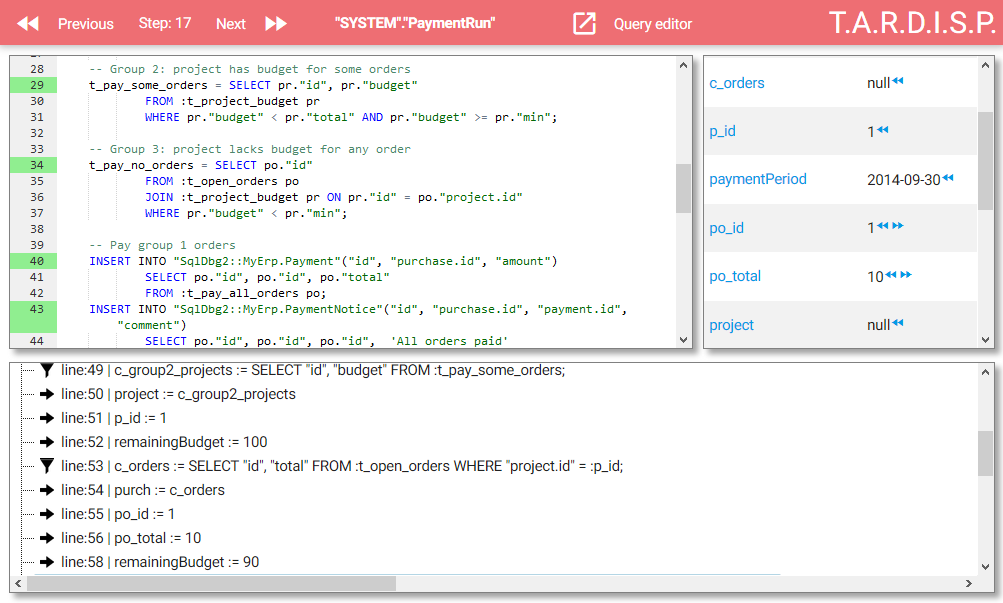
\includegraphics[width=\linewidth]{img/odb.png}
	\caption{User interface of the \tool\ debugger.}
	\label{fig:odb}
\end{figure}

The user interface looks like a typical debugger and is shown in \cref{fig:odb}.
The top-left part of the screen shows the code.
Above, a toolbar contains buttons allowing developers to step forward and backward.
Between the step buttons, the current step number is shown.
Below, \tool\ shows a tree of all execution steps instead of a stack trace.

Next to the code, current variable values are shown.
Arrow buttons allow to jump to the previous or next assignment of the variable.
For variables containing a query result, the size of the result is shown.
Clicking the variable opens a query window that shows the variable's content and allows the developer to submit time-travel queries, which will be explained in the next section.

\section{Back-in-Time SQL}



\newcommand{\red}[1]{\textcolor{DarkRed}{#1}}
\newcommand{\gr}[1]{\textcolor{Green}{#1}}
\newcommand{\timediffresult}{
\begin{table}%
	\begin{tabulary}{\textwidth}{RRRRRRR} \toprule %rlrrrlr
	%pr.id & pr.name 	& pr.budget  & total & po2.id & po2.status & po2.total \\ \midrule
		\multicolumn{3}{c}{pr.} & \multicolumn{1}{c}{po.} & \multicolumn{3}{c}{po2.} \\
	\cmidrule(lr){1-3} \cmidrule(lr){4-4} \cmidrule(lr){5-7}
	~id & name & budget  & total & ~id & status & total \\ \midrule
	
				&					  & \red{1200} & \red{1500} &	  & \red{open} &					\\
	1			& Project 1 & 200			 	 & 500 			  & 1 & paid 			 & 1000			\\
				&						& \gr{-300}  & \gr{0}		  &	  &						 &					\\ \midrule

				&					  & \red{1200} & \red{1500} &	  & 					 &					\\
	1			& Project 1 & 200				 & 500 			  & 2 & open 			 & 500			\\
				&						& \gr{-300}  & \gr{0}		  &	  & \gr{paid}	 &					\\ \bottomrule
	\end{tabulary}
	\caption{Result of a time-diff query, with multiple values in some columns. Red indicates a different value at the \emph{before} step, green indicates a different value at the \emph{after} step.}
	\label{tab:diffresult}
\end{table}
%\ctable[caption={Result of a time-diff query, with multiple values in some columns. Red indicates a different value at the \emph{before} step, green indicates a different value at the \emph{after} step.},label=tab:diffresult,doinside={\small}]
				%{rlrrrlr}{}{
	%pr.id & pr.name 	& pr.budget  & total & po2.id & po2.status & po2.total \ML
	%
				%&					  & \red{1200} & \red{1500} &	  & \red{open} &					\NN
	%1			& Project 1 & 200			 	 & 500 			  & 1 & paid 			 & 1000			\NN
				%&						& \gr{-300}  & \gr{0}		  &	  &						 &					\ML
%
				%&					  & \red{1200} & \red{1500} &	  & 					 &					\NN
	%1			& Project 1 & 200				 & 500 			  & 2 & open 			 & 500			\NN
				%&						& \gr{-300}  & \gr{0}		  &	  & \gr{paid}	 &					\ML
%}
}
%\newcommand{\timediffresult}{
%\ctable[caption={Result of a time-diff query, with multiple values in some columns. Red indicates a different value at the \emph{before} step, green a different value at the \emph{after} step.},label=tab:diffresult,doinside={\small}]
				%{rrrrrrr}{}{
	%\multicolumn{3}{c}{pr.} & \multicolumn{1}{c}{po.} & \multicolumn{3}{c}{po2.} \NN
	%\cmidrule(lr){1-3} \cmidrule(lr){4-4} \cmidrule(lr){5-7}
	%id & name & budget  & total & id & status & total \ML
	%
				%&						& \red{1200} & \red{1500} &	  & \red{open} &					\NN
	%1			&	Project 1	& 200			 	 & 500 			  & 1 & paid 			 & 1000			\NN
				%&						& \gr{-300}  & \gr{0}		  &	  &						 &					\ML
%
				%&						& \red{1200} & \red{1500} &	  & 					 &					\NN
	%1			&	Project 1	& 200				 & 500 			  & 2 & open 			 & 500			\NN
				%&						& \gr{-300}  & \gr{0}		  &	  & \gr{paid}	 &					\ML
%}
%}

\tmpStart

In our setup, the debugger has to recreate intermediate results of a stored procedure.
We generalized this feature to enable developers to submit arbitrary queries against the database of any previous point in time.
Furthermore, we allow developers to compare query results from different points in time and even query for changes in the data.
We defined \SQLextension, a super-set of SQL introducing a new keyword and a new operator.

\subsection{A SQL Clause to Query Points in Time}

As an example, we consider a stored procedure that triggers the payment of purchase orders.
Users reported a bug: projects sometimes exceed their budget, which is not supposed to happen.
Developers might start debugging this issue and the related stored procedure with \tool.
However, they soon realize that the number of projects is too large to continue stepping manually.
Instead, they open \tool's SQL console and submit the query shown in \cref{lst:ttravel} to look into the ´select_projects´ variable, which contains ids, names, and budgets of all projects to be processed.
To better understand the data, they also sum up the total amount of all open purchase orders for each project.

%\Cref{lst:ttravel} shows the query to fetch all selected projects together with the total amount of open orders\todo{The previous paragraph already explains the code - reference to listing needs to be earlier.}.
%We will use it as an example to show how \tool\ handles time-travel queries.

%\begin{figure} % IEEE says put code in figures
%\begin{lstlisting}
\begin{lstlisting}[language=HanaSQL,float,caption={Example for a time-travel query: select the current total of open orders for previously selected projects at step 1623 of the execution},label=lst:ttravel]
  SELECT pr.id, pr.name, pr.budget, SUM(po.total)
  FROM :selected_projects pr
	JOIN PurchaseOrders po ON po.project_id = pr.id
	WHERE po.status = 'open'
	GROUP BY pr.id, pr.name, pr.budget
	^§AT STEP§ 1623^
\end{lstlisting}
%\caption{Example for a time-travel query: select the current total of open orders for previously selected projects}
%\label{lst:ttravel}
%\end{figure}

The last line of \cref{lst:ttravel} contains the ´^AT STEP^´ clause, our extension to SQL that allows developers to explicitly query a specific point in time.
When opening the SQL console, \tool\ automatically provides an ´AT STEP´ clause with the number of the current debug step, ´^1623^´ in this case.
Developers can obtain numbers for other steps from the stepping toolbar or the execution tree. 

When the query is submitted, \tool\ applies two transformations before it is passed to the database.
First, all variables are replaced with their corresponding functions or views that were generated during the pre-processing of the stored procedure.
Each function or view receives the specified step number as an argument to be able to produce the correct value or table.
Second, time-stamp filters on the validity columns are added for all tables that are referenced in the query. 
%Because of SAP HANA's insert-only approach, 
This lets all tables appear exactly as they originally were at the specified point in time.

%In our example,
%\begin{lstlisting}[language={Inline},basicstyle=\ttfamily,numbers=none]
  %po.createdOn < ^1623^ AND (po.validTo IS NULL OR po.validTo > ^1623^)
%\end{lstlisting}
%would be added to the where-clause.

Now, the query can be submitted to the database and the result is subsequently presented to the user.

When developers omit the step number, it is taken from the context of the debug session.
This way, developers can step through the execution and observe how the query result changes over time.

\subsection{Time-diff Queries}

Furthermore, \SQLextension\ provides an easier way to find the origin of changes in the data.
To get a better overview about what happened in a segment of code, developers might want to query multiple points in time at once and see the difference in the query result.
In our example, developers are looking for purchase orders that cause projects to exceed their budget.
Using \tool, they identified three important points in time, which we will call \emph{before}, \emph{now}, and \emph{after}.
\emph{Before} is the step where the stored procedure started processing purchase orders, \emph{now} is the current step, and \emph{after} is the final step of the procedure.

In \cref{lst:tdiff}, the query from above was extended to select individual purchase orders for each project.
In line 10, the at-step clause now specifies all three points in time.
This allows developers to query for changes in the data.

Because the steps are named, they can now be used in the query as time qualifiers.
\SQLextension\ introduces the exclamation mark operator that binds an identifier to a step.
In line 6, it is used to limit the search to projects that will exceed their budget before the stored procedure ends;
in line 7, it is used to filter for purchase orders whose status was or will be changed.

%\begin{figure} % IEEE says put code in figures
%\begin{lstlisting}
\begin{lstlisting}[language=HanaSQL,float=t,caption={Example of a time-diff query: "Select all projects that will go over budget and their respective purchase orders"},label=lst:tdiff]
	SELECT pr.id, pr.name, pr.budget, SUM(po.total), po2.id, po2.status, po2.total
	FROM :selectedProjects pr
	JOIN PurchaseOrders po ON po.project_id = pr.id
	JOIN PurchaseOrders po2 ON po2.project_id = pr.id
	WHERE po.status = 'open'
		AND ^now!^pr.budget > 0 AND ^after!^pr.budget < 0
		AND ^before!^po2.status != ^after!^po2.status
	GROUP BY pr.id, pr.name, pr.budget, 
	         po2.id, po2.status, po2.total
	^§AT STEP§ before=817, now=1623, after=2043^
\end{lstlisting}
%\caption{Example of a time-diff query: "Select all projects that will go over budget and their respective purchase orders"}
%\label{lst:tdiff}
%\end{figure}
\timediffresult
\Cref{tab:diffresult} shows a possible result for this query, with one project that goes over budget and two associated purchases.
The values for budget and total of outstanding payments are shown for each of the three steps.
Of the two purchase orders, the first was already marked as "paid" before the current step, the other is about to be paid.

Analyzing this data, it becomes clear that the payment of the second order is what causes the project budget to become negative.
Developers can now click on the green "paid" value to jump exactly to the point in time where this order is updated, knowing that at this point they are very likely to be close to the defect they are looking for.

To produce this result, the query has to be executed three times, once for each point in time, without the time-specific where-conditions.
The partial results are outer-joined on the primary key attributes, then the time-specific filter conditions are applied.
\tool\ rewrites the query to fit everything into a single select statement, which allows the database to compute the entire result in one request.

%The final query selects all values from each sub-query.
In the user interface, changes in the values are highlighted in as shown in \cref{tab:diffresult}.
If a value changed since the \emph{before} step, the old value is shown in red; if a value will change until the \emph{after} step, the new value is shown in green.
When possible, the tuple creation timestamps are used to allow developers to jump exactly to the point in time where the change occurred.

%Then, to prepare the diffing of the results, they are outer-joined on the primary keys and the time-specific filters are applied.
%For performance reasons, all of this happens inside a single SQL query, as shown in \cref{lst:tdifffinal}.
%The execution of the sub-queries is indicated in \linerefn{lst:tdifffinal}{6, 7, and 10}, the time-specific filters can be found in the Where-condition of \linerefn{lst:tdifffinal}{15 and 16}.

%
%In the UI\todo{Instead of many code listing show the UI (this could also include the code)}, the before and after values are only shown if they differ from the now value.
%Clicking on value allows the developer to jump to the ´UPDATE´ or ´INSERT´ statement that caused the change.


\section{Performance Evaluation and Developer Interviews}

\tmpStart

%\ctable[caption=,label=tab:measure1,doinside={\small},width=\linewidth]
				%{lc>{\raggedleft \arraybackslash}p{1.3cm}RR}{}{
				%&		& Normal run& Run with tracing  & Reproducing the result \ML
	%
			 %&	(a) &	1.27 s		& 1.35 s		& 1.21 s		\NN
%Proc. 1& (b)	&	1.61 s		& 1.74 s		& 1.54 s		\NN
			 %&	(c) &	1.73 s		& 1.85 s		& 1.60 s		\ML
%
			 %&	(a) &	1.24 s		& 1.32 s		& 1.19 s		\NN
%Proc. 2& (b)	&	1.61 s		& 1.72 s		& 1.55 s		\NN
			 %&	(c) &	1.69 s		& 1.80 s		& 1.63 s		\ML
%}

\begin{table}
	\centering
	\begin{tabulary}{\textwidth}{lcRRR}
	\toprule
				&		& Normal run& Run with tracing  & Reproducing the result \\ \midrule
	
			 &	(a) &	1.27 s		& 1.35 s		& 1.21 s		\\
Proc. 1& (b)	&	1.61 s		& 1.74 s		& 1.54 s		\\
			 &	(c) &	1.73 s		& 1.85 s		& 1.60 s		\\ \midrule

			 &	(a) &	1.24 s		& 1.32 s		& 1.19 s		\\
Proc. 2& (b)	&	1.61 s		& 1.72 s		& 1.55 s		\\
			 &	(c) &	1.69 s		& 1.80 s		& 1.63 s		\\ \bottomrule
	\end{tabulary}
	\caption{Average execution time for running a stored procedure without and with tracing and for reproducing its result.}
	\label{tab:measure1}
\end{table}

\begin{table}
	\centering
	\begin{tabulary}{\textwidth}{lcRR}
	\toprule
				&		& Regular query& Time-diff query \\ \midrule
	
			 &	(a) &	1.21 s		& 1.51 s	\\
Query 1& (b)	&	1.74 s		& 2.12 s	\\
			 &	(c) &	1.79 s		& 2.23 s	\\ \midrule

			 &	(a) &	61 ms		&  75 ms	\\
Query 2& (b)	&	81 ms		& 100 ms	\\ 
			 &	(c) &	88 ms		& 109 ms	\\ \bottomrule
	\end{tabulary}
	\caption{Average execution times for queries executed normally or as time-diff query.}
	\label{tab:measure2}
\end{table}

%\ctable[caption={Average execution times for queries executed normally or as time-diff query.},label=tab:measure2,doinside={\small},width=\linewidth]
				%{lcRR}{}{
				%&		& Regular query& Time-diff query \ML
	%
			 %&	(a) &	1.21 s		& 1.51 s	\NN
%Query 1& (b)	&	1.74 s		& 2.12 s	\NN
			 %&	(c) &	1.79 s		& 2.23 s	\ML
%
			 %&	(a) &	61 ms		&  75 ms	\NN
%Query 2& (b)	&	81 ms		& 100 ms	\NN
			 %&	(c) &	88 ms		& 109 ms	\ML
%}

We evaluated our \tool\,debugger on a real-world SAP project that has been developed with one of the largest European retail companies. 
This project is called \emph{Point of Sales Explorer}~\cite{plattner15:the_in-memory_revolution_how} and allows category managers to see a collection of the most important key performance indicators (KPIs) for several thousands of products in a unified dashboard.
Based on more than 2 billion records of point of sales data, this application aggregates on the fly the requested KPIs with the help of SAP HANA and allows users to further refine them by stores, vendors, or products as they like. 
In order to implement flexible requests such as returning the revenue and margin per week of current and last year, this application makes heavy use of SQLScript. 
For that reason, it is a proper candidate to measure performance and interview its developers with respect to our \tool\ tool. 

\subsection{Performance Measurements}

To evaluate the performance of our approach, we deployed \tool\ on a copy of the productive system.
We selected two stored procedures from the Point of Sales Explorer and compared the runtime with and without tracing.
To measure the impact of database size, we ran each procedure with different arguments that would lead to intermediate results of different sizes.
Each value is the average of ten measurements.
%The results are shown in \cref{tab:measure1}.
As \cref{tab:measure1} shows, we found the overhead of tracing to be consistently between six and seven percent.

We also measured the time it takes to reproduce the results of each stored procedure.
This provides us with an upper bound for how long \tool\ would need to compute the value of any variable because in our examples all variables are needed to compute the final result.
The measurements in \cref{tab:measure1} show that reproducing the result is slightly faster than executing the stored procedure.
This was expected because for variables containing atomic values the value could be taken directly from the trace.
Only for variables containing table results, database queries had to be executed again.

Finally, we selected two queries from the stored procedures as examples a developer might submit through the debugger's SQL console and measured their execution time both as a regular query and as a time-diff query.
%Because the Point of Sales Explorer onlyu computes KPIs and does not change the data, we let the time-diff query compare different time-spans of point of sale data\todo{is this disclaimer needed?}.
Again, we used different filter arguments to produce different result sizes.
As \cref{tab:measure2} shows, in each case the runtime overhead of time-diff queries is around 25 percent.

Developers will avoid tools that are too slow to allow fluent working because every delay distracts from the problem to be solved. 
Back-in-time debuggers often suffer from this problem.
Our measurements show that the overhead created by \tool\ is small enough to make it a feasible alternative to existing debugging tools.

\subsection{Interviews}

Besides measuring performance, we also demonstrated our back-in-time debugger to two backend developers of the Point of Sales Explorer. 
These persons have written most of the SQLScript and so know all the challenges when developing close to the database. 
Both had the chance to apply \tool\ in their daily work while we provided tool support and observed them in the background. 
Finally, we have conducted an in-depth interview in order to receive feedback and further improve our tool.

We found out that the main reason for writing SQLScript is to positively influence the optimizer of SAP HANA in order to speed up the overall user request.
If something went wrong at the database-level, the existing tool support was not sufficient. 
The interviewed developers often had to guess why a specific sub-query was not return the expected results. 
%For that reason, they liked our back-in-time debugger and we received a lot of positive feedback.
For this, they liked \tool\ as it could not only show formerly hidden results but also helped them to understand and follow back the reasons behind a failure cause. 
The greatest improvement was reported for debugging stored procedures that take a table of data as an argument, whose cumbersome preparation has to be done only once, using \tool.
Composing such an argument with specific data using the existing tools is cumbersome and has to be redone every time the debug session has to be restarted.
Using \tool, it has to be done only once.
Besides that, both developers wished for some new features such as the ability to define temporary tables for testing code and queries.
With this feedback, we see a strong need for better debugging support at the database-level and are eager to further improve our approach.

%We found out that the main reason for writing SQLScript is to positively influence the optimizer of SAP HANA in order to speed up the overall user request.
%This worked very well as long as the newly written code was free of failures. 
%However, if something went wrong at the database-level, the existing tool support was not sufficient. 
%The interviewed developers often had to guess why a specific sub query was not return the expected results. 
%For that reason, they liked our back-in-time debugger and we received a lot of positive feedback.
%For example, \tool\ could not only show formerly hidden results but also helped them to understand and follow back the reasons behind a failure cause. 
%The greatest improvement was reported for debugging stored procedures that take a table of data as an argument.
%Composing such an argument with specific data using the existing tools is cumbersome and has to be redone every time the debug session has to be restarted.
%Using \tool, it has to be done only once.
%Besides that, both developers also revealed several small failures in our debugger and wished for some new features such as the ability to define temporary tables for testing code and queries.
%With this feedback, we see a strong need for better debugging support at the database-level and are eager to further improve our approach.

%\subsection{Threats to Validity}

\subsection{Limitations}

Our implementation of \SQLextension\ currently has two limitations.

First, time-diff queries can only be executed on tables that have clearly defined primary keys because key attributes are required to track a tuple's version over time.
For a query like "Sum budgets per project category", it has to be clear that categories are the entities that keep their identity over time.
Here, an additional syntax extension could be used to convey this kind of information.

Second, it is currently not possible to use time qualifiers on identifiers outside of the where clause.
We can imagine that there may be a need to use time qualifiers in other SQL clauses, such as the select or order-by clause.
In other use cases, developers might want to attach a time qualifier directly to a table.



\tmpEnd

\chapter{Omniscient Debugging Across System Boundaries}


%\section{A System-independent View on Debugging}
%
%\section{Detecting Inter-System Program Flow}

\tmpStart

\section{Introduction}
\label{sec:introduction}

% Context: architectures
Complex applications are rarely single programs running on a single machine but often consist of multiple components implemented in different programming languages and running in different environments.
A notable example is the multi-tier architecture, a successful and established pattern for client-server applications since over two decades.

% Problem
Breaking down applications into layers and sub-systems allows for better scalability and easier life-cycle management, but makes debugging such applications much harder.
Software failures are typically observed in the front-end first.
Then, developers have to guess which layer contains the fault. 
Otherwise, they have to switch debugging tools frequently while they track the infection chain across the entire software stack.

% Signifiance
In the past, this problem was mitigated because most application code resided in the business tier, while the presentation and data tiers only served to display back-end provided views and to persist application state, respectively.
However, changes in technologies and requirements caused more code to move up or down the stack, thereby increasing the need to debug the application as a whole.
Service-oriented architecture and micro-services are more recent patterns that exacerbate the problem by dividing applications into even more independent components.

% Solution
We interviewed software developers on the difficulties when developing modern enterprise applications.
Based on these insights, we developed a prototype for a back-in-time debugger allowing developers to debug the full stack of a 3-tier application in one session.

Assuming back-in-time debugging capabilities for each application tier, we introduce hierarchical step numbering based on synchronization points between components to create a partial ordering of instructions in all concurrent executions.
A visualization shows which UI element is affected by which back-end operation, providing developers with a top-down summary of the execution.
A second visualization is shown in the debugger and helps developers to navigate the application flow.

We then collected developer feedback for our prototype.
Based on this feedback, we identified suggestions how existing debugging tools can be improved even without the need for resource-intensive back-in-time debugging.

The remainder of this paper is structured as follows:
The next section summarizes related work.
\Cref{sec:interviews} discusses the results of our interviews. 
We describe in more detail how 3-tier applications have changed in the last decade and which information developers need when debugging such applications.
\Cref{sec:debugger} presents our prototype implementation of a full-stack back-in-time debugger.
\Cref{sec:conclusion} concludes.

%\section{Related Work}
%
%%The concept of slicing was introduced by Weiser and initially only built on static analysis \cite{weiser_programmers_1982, weiser_program_1981}.
%%Later, Korel and Laski \cite{korel_dynamic_1990} and Agrawal and Horgan \cite{agrawal_dynamic_1990} introduced dynamic slicing by proposing different ways of extending the concept to the run-time.
%
%The idea of being able to debug backwards in time dates back to the 1960s with EXDAMS, a debugger for FORTRAN \cite{balzer_exdams_1969}.
%Since then, debuggers with back-in-time capabilities have been implemented for many programming languages \cite{agrawal_debugging_1993, feldman_igor_1988, lieberman_zstep_1997}.
%
%In 2003, Lewis introduced the concept of "omniscient debugging", a debugger that can not only rewind time, but has instant access to every point in past and future~\cite{lewis_debugging_2003}.
%Later work on omniscient debugging focused mostly on handling the large amounts of data such a debugger creates~\cite{pothier_scalable_2007, lienhard_practical_2008}.
%Perscheid et al. \cite{perscheid_testdriven_2013} combined omniscient debugging and spectrum-based fault analysis, analyzing a suite of unit tests with passing and failing test cases.
%%Perscheid et al. \cite{perscheid_test-driven_2013} combined omniscient debugging and dynamic code analysis similar to slicing to automatically identify likely locations for code defects by analyzing a suite of unit tests with passing and failing test cases.
%
%Lanza showed the importance of visualizations in software development~\cite{lanza2003program}.
%SHriMP views are one example how such visualizations can guide developers~\cite{storey2002shrimp}.
%Baecker et al. used visualizations to improve the debugging process by animating algorithms~\cite{baecker1997software}.
%Moher~\cite{moher1988provide} and Beguelin et al.~\cite{beguelin1993visualization} used visualizations to support the understanding of process interactions in heterogeneous environments.
%However, in both works the focus was set more on understanding and debugging applications on an architectural level, while we aim to integrate debugging of individual components as if the software was a single program.
%
%%SPYDER is a debugger with slicing and back-and-time capabilites \cite{agrawal_debugging_1993}.
%%With SPYDER, Agrawal et al. also proposed a new debugging workflow that is similar to our approach.
%%However, while Agrawal et al. proposed to create a new slice every time the programmers question changed, our approach focuses on iteratively modifying a single slice.
%%Furthermore, we present a new way of presenting aspects of the slice to developers.
%Our approach requires that searchable traces are available for all sub-systems of an application.
%Solutions for collecting and storing execution traces always depend on the underlying technology, nevertheless some general approaches exist.
%Mellor-Crummey and LeBlanc showed how to obtain instruction pointers in software when they are not provided by the system, which is a general requirement for tracing~\cite{mellor-crummey_software_1989}.
%With PQL, developers can search for the occurrence of code examples in program executions~\cite{martin_finding_2005}.
%Similarly, Recon is a debugging tool that allows to query the execution of distributed systems with SQL-like queries~\cite{lee_unified_2011}.
%Recon's query interface can not only provide all the information a debugger would need.
%O'Callahan et al. presented a generic approach for recording and replaying program executions~\cite{ocallahan_engineering_2017}.
%
%
%
%
%\section{Developer Needs in Debugging Modern Client-server Applications}
%\label{sec:interviews}
%
%To better understand the development of modern business software, we interviewed five software developers from SAP, a German software corporation developing enterprise software to manage business operations.
%From these developers, we gained insights on the development of four different projects:
%\begin{enumerate}
	%\item A software for liquidity risk management that analyzes the cash-flow of financial institutes to assess their liquidity,
	%\item A customer analytics software to understand customer behavior based on collected data, which allows, for example, to identify particularly profitable customers or customers that plan to leave the company (e.g., clients of a bank who cancel all their standing orders),
	%\item A product for predictive analytics that allows to estimate the probabilities for certain customer behaviors, such as switching distributors or suppliers. The analyses' results are integrated in a customer relationship management (CRM) system and recommend opportunities for salespeople, and
	%\item The point-of-sales (POS) explorer, a dashboard that computes various key performance indicators (KPIs) on the revenue and profits of products based on retail data.
%\end{enumerate}
%%
%All applications are designed to work on real-time data generated by respective transactional systems and were developed with an industry partner who provided requirements.
%
%\subsection{Changing Characteristics in 3-tier Applications}
%
%The design of all applications was based on the 3-tier architecture pattern, which divides an application into three layers~\cite{eckerson_95_three_tier_clientserver_architecture}.
%The \emph{presentation tier} displays information and receives input from the user,
%the \emph{application tier} contains the application's business logic, and
%the \emph{data tier} encapsulates data access and persistence.
%The presentation tier is the application's front-end and runs on the client, while the application and data tier constitute the back-end and run on the server.
%
%In traditional 3-tier applications, most of the code is implemented in the application layer.
%For example, templates allow the application server to render web pages that can be displayed by a browser on the client.
%When a dedicated client application is needed, keeping it small and simple reduces the overhead of maintaining and updating a large number of installations.
%Either way, the client is little more than a terminal.
%
%On the data side, object-relational mappers (ORMs) allow developers to implement data processing logic directly in the application.
%This makes applications independent from specific database products and avoids introducing additional programming languages into the project.
%Because application servers can be scaled more easily than databases, this also reduces the database bottleneck that can occur in applications with many users.
%
%Many application frameworks, such as J2EE and Ruby on Rails, follow this philosophy and many tools have been developed to support development and maintenance in such ecosystems.
%However, as we found in our interviews, the usefulness of many of such tools is decreasing as technologies and requirements change in the development of modern business applications.
%
%HTML 5 and JavaScript allow to build responsive and dynamic interfaces, which are increasingly expected by users.
%Via HTTP and fast connections, megabytes of client code can be updated with every request so there is no longer a need to keep the client code minimal.
%JavaScript-based GUI libraries eliminate the need for server-side templates as the entire GUI can be built in the client and data is dynamically loaded via AJAX requests.
%
%With big-data becoming more important for many companies, it is no longer feasible to handle all data operations in the application layer.
%Even transactional systems contain a large fraction of analytical operations~\cite{krueger_case_2010} and high-performance databases can handle such queries faster than application-level code~\cite{plattner_common_2009}.
%Even for transactional operations, the usefulness of ORMs is doubted as they can introduce other organizational and architectural problems~\cite{neward_vietnam_2006}.
%
%All developers reported that their projects followed these new architecture patterns.
%To achieve sufficiently low response times, data is stored in \emph{SAP HANA}, a high-performance in-memory relational database.
%The application layers run in \emph{SAP HANA Extended Application Services}, an application and web server environment on top of the database.
%In each project, the front-end is implement in \emph{SAPUI5}, a JavaScript GUI library based on jQuery.
%
%For the fourth project, the POS explorer, we were given full access to the code base.
%At the time of the interview, the whole application had 11 thousand lines of code, libraries excluded.
%55\% of the code (i.e., about 6000 lines) was client-side JavaScript, of which about 12\% (725 lines) was data querying code.
%The application layer consisted of 2000 lines (18\%) of server-side JavaScript (similar to node.js), while the database layer contained 3000 lines (27\%) of stored procedure code.
%Data schema definitions are not included in the line counts, as the data is defined and provided by other applications.
%% client/js					2397
%% client/fragment		3750
%% client/view				 133
%% client -- query		 600 // client 6280 -- 6000
%% app/xsjs*					2250 //  -- 2000
%% db/procedure			2991 // -- 3000
%% // 11521
%
%Standards like \emph{OData}~\cite{chappell_introducing_2011} allow clients to submit arbitrary queries to the database, entirely eliminating the need for a middle layer.
%It should be noted that this setup is different from the classical 2-tier architecture, where a trusted client has full access to the database.
%OData still maintains security concerns such as authentication, authorization, and visibility of data, which was previously a responsibility of the application tier.
%
%For one of the projects, the developer reported that they have no application layer code at all.
%The application, he estimated, consisted of 90\% client-side JavaScript, of which one-third was OData client code, and 5\% OData service configuration which passed requests to stored procedures that constituted the remaining 5\% of the project.
%
%In conclusion, due to increased complexity of interactions between the different layers it is no longer sufficient to be able to debug each layer on its own.
%Instead, tools are needed that help developers to debug and understand the application as a whole.
%
%\subsection{Debugging 3-tier Business Applications}
%
%All developers reported that changes in software development processes affected the way how bugs are handled.
%In the past, large applications had separate development teams for front-end, business logic, and data management.
%If a team found that a bug was not caused in their respective domain, the responsibility was passed on to the next team.
%
%Agile development methodologies, such as Scrum or Extreme Programming, discourage dividing teams by technology layer.
%Instead, requirements and, if necessary, sub-teams are now grouped around feature sets.
%Thus, while there still may be developers who are specialized on one of the application tiers, every developer is expected to be able to work on and to debug every layer.
%This increases the need for making debugging tools for each layer easily available to all developers.
%
%The existence of bugs is typically discovered by observing unexpected data in the user interface.
%Then, developers use their browser's development tools to examine the request with which the data was obtained.
%In most cases, the response data is passed unchanged to the GUI components and the incorrect data can be tracked directly back to the response.
%Here, the first uncertainties occur as it is often not obvious whether the request was submitted with incorrect arguments or whether the error is on the server-side.
%
%If developers decide to continue to the application code, they determine which server function is called, connect a debugger to the application server, set a breakpoint, and re-submit the failing request.
%Then they use the debugger to understand how the request is processed.
%
%If no fault can be found, they now need to determine if the results returned by database queries are correct.
%For queries that include complex views or stored procedures, this is not an easy task.
%Furthermore, if the query was composed at runtime, developers also need to determine the actual query string and which arguments were used.
%After that, they can use the tools provided by the database client to analyze the query and verify the result.
%
%Using these methods, developers move up and down the stack until they find the root cause of the bug.
%Generally, all developers reported that they preferred to work with a top-down approach, i.e., they try to first understand the interaction between the layers before starting a debugger to narrow down possible locations for the bug as early as possible.
%However, while the developer tools of browsers were reported to be somewhat useful for this task, no such tools exist to understand the interaction between application and data tier at a glance.
%
%Overall, frequent switches between tools were reported to be a major distraction when trying to focus on the program flow.
%Often, multiple monitors were used to allow developers to access all tools more quickly, but all developers wished for better integration between tools.

\section{A Prototype for Full-stack Back-in-time Debugging}
\label{sec:debugger}

Based on the collected developer experience, we built a back-in-time debugger for 3-tier applications running in SAP HANA.
%We tested the debugger on the POS explorer and were able to seamlessly debug the entire application stack, while providing additional high-level visualizations

\subsection{Obtaining the Full Execution History}

For the purpose of our debugger, we assume that omniscient debugging capabilities for each layer already exist.
This means that we need not only the ability to move execution forwards and backwards, but also a way to search the entire history for specific instructions.
At the very least, we need a way to obtain full traces of all layers that we can store in a database.

In this context, we call an \emph{execution} the invocation of a function or method in a layer that was triggered by an external event, such as a request or a response from a different layer, and that is traced independently of other previous, concurrent, or future executions.
The \emph{full execution history} is the set of all executions that were transitively caused by a root execution.
In the full history, multiple executions that may appear to be independent are grouped together as they are part of the same higher-level operation.

To be able to fully restore the program state from any point in time, traces need to contain not only all method invocations, but also all variable assignments and all field accesses.
For the technologies involved, no tracing tools that could provide the required level of detail existed at the time.

For the data layer, we used our existing omniscient debugger for stored procedures.%~\cite{treffer2017bringing}.
It inserts trace statements into the code that save the execution in the database.

In the application layer, the server runtime needs to collect and store the trace.
Since the SAP HANA platform has no such capabilities at this time, we used a similar approach as with the stored procedures debugger.
A pre-processor parses the JavaScript files and inserts trace statements for all instructions.
Then, to collect a trace, the actual back-end code has to be temporarily replaced with the modified tracing code.

In the front-end, the browser or a browser plug-in can be used to collect the execution trace.
However, while there exist many tracing plug-ins for all modern browsers, most are designed for performance profiling and therefore don't provide the necessary level of detail.
We also found that many browsers provide a debugging interface that could be used to implement a tracing plug-in.
Nevertheless, for now we again used our JavaScript pre-processor.
For simplicity, we only traced the application code and not the SAPUI5 and jQuery libraries.

Both the front-end and the back-end JavaScript tracer first store the entire trace in an array and then, at the end of the execution, submit it to the database.
From the front-end, data is sent via an HTTP POST request and then passed on to the database via a back-end script.
All JavaScript execution traces are stored in a single relational database schema, the execution traces of stored procedures are stored in a second, slightly different schema.

In the POS explorer, drop-down boxes allow to select filter criteria that are then applied to all components on the dashboard.
\Cref{fig:pos} on page~\pageref{fig:pos} shows a section of the user interface.
The green and red boxes were inserted by our debugger and can be ignored for now.
Selecting, for example, "BACONSNACKS" from the category drop down at the top of the screen updates five UI components of which three are shown in \cref{fig:pos}.

In total, this operation generates almost 400 traced instruction in the back-end, libraries excluded.
Due to the asynchronous nature of AJAX requests, those events are split over 5 separate executions.
Four HTTP requests to the back-end create four executions with around 800 traced instructions each.
Each back-end request triggers one stored procedure, each with 17 to 25 traced instructions.

\subsection{Identifying Sub-system Interactions}

When all operations have completed, we have traced a total of 13 executions.
To allow seamless debugging of the entire application, we now have to restore the request/response relations that define the application flow.
Since most requests are handled concurrently, we can not simply use timestamps to recreate the order.

In a first step, we select all executions from the trace databases that occurred in the time-frame of the front-end operation and number them in order of the time stamp of the first recorded instruction.
Then we create a mapping between execution number and its schema and the execution id within that schema.
This mapping will later be needed for uniquely identifying each point in time while allowing for sequentialized debugging of concurrent executions.

In the second step, we collect all requests that were sent from each layer.
This step is technology-specific.
For the front-end, we scan the trace database for invocations of ´jQuery.ajax()´ and determine the request URL to later identify the request.
In the application layer we scan for invocations of ´execute()´ on prepared-statement objects and determine the query string.

In both cases, our prototype was specifically tailored for the POS explorer.
First, there are many different ways in which a request can be sent and we covered only the ways that were actually used.
Second, when determining the URL and query strings we took advantage of the fact that the strings were always stored in a variable of the same name.
For a generalized solution, the debugger needs to perform a small dynamic code analysis to identify the correct values.
With full access to the code and the execution trace, this analysis should not be too difficult to perform, but for now it was beyond the scope of our project.

In the third step, we determine for each execution by which request it was triggered.
In the application layer, we inserted special tracing code to record the request URL, which then only has to be matched against the URLs requested by the front-end.
To match stored procedure calls, we check which query string contains the procedure name as a sub-string.
Finally, four executions in the front-end were triggered by asynchronous AJAX results.
Here, we used the fact that the response is handled in the same file from which the request was sent to find the original request.

In the case of the POS explorer, this was enough to unambiguously match all request and response relations.
In other scenarios, where multiple very similar requests are sent, other approaches may be needed.
For example, unique arguments could be added to request URLs to allow for better matching of executions.
In the case of database requests, the runtime environment probably has better ways of matching requests, such as internal connection ids.
With a better integration of tracing in the platform, such data can be easily recorded and used accordingly.

\subsection{High-level Visualizations}

% component11
% component13
% component14
% component15

All developers we interviewed reported that they prefer to begin debugging by understanding the high-level interactions first.
Now that the debugger can successfully identify these interactions, they can be visualized in the user interface.
Our prototype provides two visualizations.

First, calls to the back-end layers are shown directly on the web page, right next to each UI component, as shown in~\cref{fig:pos}.
This allows developers to immediately see which request belongs to which component, which is particularly helpful if only one component shows incorrect data.

\begin{figure}
	\centering
		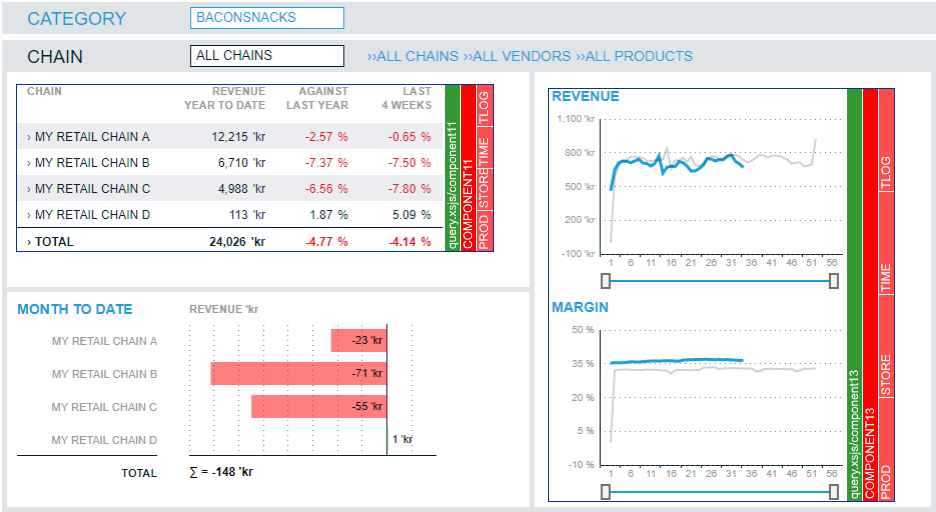
\includegraphics[width=1.00\linewidth]{img/pos.png}
	\caption{A section of a KPI dashboard. Directly next to UI components, elements were inserted that show which back-end functions and data sources provided the displayed data.}
	\label{fig:pos}
\end{figure}

In our prototype, mapping requests to UI components is possible because we can track from which component's ´refresh()´ method the request was sent.
As can be seen, the bar chart at the bottom left has no associated requests shown because it reuses data from the table above.
For a more generalized solution, code analysis can be used to determine to which UI components data is passed.
This will work even for scenarios where a central refresh method updates all components or where client-side post-processing of the data is performed.

Colors are used to show the involved application layers.
The green box shows the path of the request URL, the red boxes show the names of the stored procedures and database tables that where subsequently accessed.

Second, the debugger window, as shown in~\cref{fig:debugger}, shows a full overview of all interactions.
The largest part of the debugger windows is occupied by the source code.
To the right, current variable values are shown.
At the top of window, a diagram shows the entire history of all individual executions and their request/response relations.

\begin{figure}
	\centering
		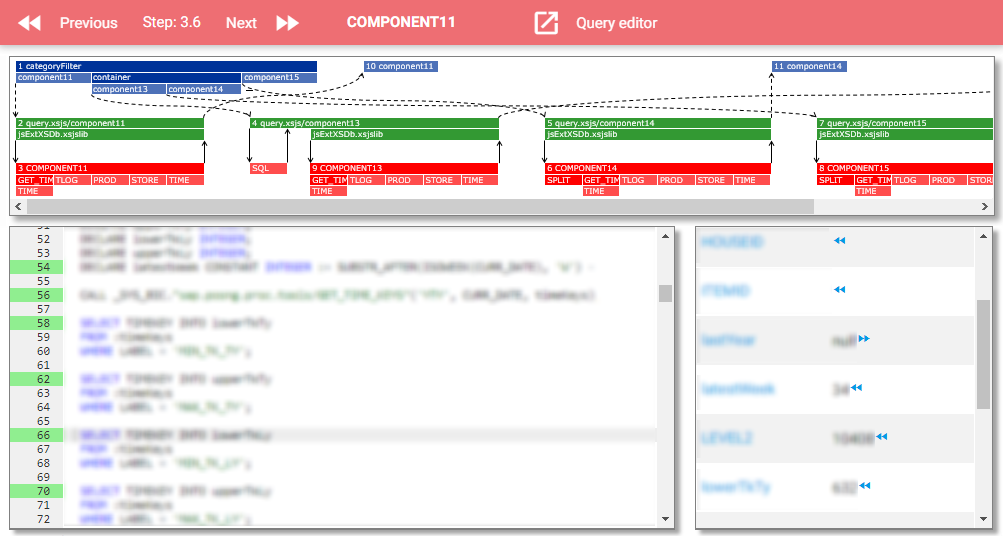
\includegraphics[width=1.00\linewidth]{img/debugger_full.png}
	\caption{A screenshot of our debugger prototype. On top of the code and variables view, a diagram shows the flow of requests in the application.}
	\label{fig:debugger}
\end{figure}

\begin{figure}
	\centering
		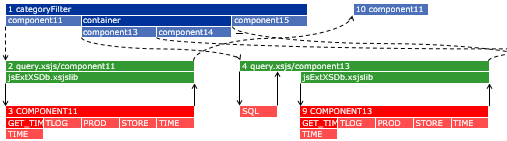
\includegraphics[width=1.00\linewidth]{img/executions.png}
	\caption{A part of the interaction diagram. Colors encode the application layer, dashed arrows represent asynchronous, solid arrows represent synchronous requests and responses.}
	\label{fig:executions}
\end{figure}

\Cref{fig:executions} shows a part of the interaction diagram in more detail, with anonymized names.
Each group of adjacent rectangles represents one execution trace.
The execution number and name are shown in the topmost rectangle of each group.

For the front-end, shown in blue, the blocks represent the hierarchy of UI components.
In the application layer, green blocks show the files that were executed to respond to requests and below files that submitted database queries.
Red blocks, finally, show the stored procedures that were called and, in lighter red, the tables that were accessed.
At the beginning of execution \#4 in the application layer, a plain SQL query is submitted to the database, not calling any procedures.

The length of the rectangles has no significance, in particular it does not reflect execution times.
Between the layers, asynchronous calls are shown with dashed lines, synchronous calls with solid lines.

The diagram is interactive.
For example, clicking the arrows reveals details about the requests.
For HTTP requests, the request URL and arguments and the response body are shown.
Clicking a database request opens a query window with the query string.
This allows developers to inspect the query result and to modify the query, which can help to better understand the data.
Finally, clicking a rectangle moves the debugger to the point in time where the respective code is executed.

\subsection{Debugging the Full Stack}

After developers have gained an overview over the full execution history and maybe formed first hypotheses about the bug, they want to begin debugging the code.
With the entire execution history recorded, a post-mortem debugger can replay the execution.

To identify a point in time, the debugger needs the execution number and the instruction index within the execution.
From the execution number, the debugger resolves which trace database to use.
Then, with the instruction index the current code location and program state is restored.
Stepping forwards and backwards changes the instruction index within the execution.

Typically, a back-in-time debugger allows to step forwards and backwards within a method and into and out of method calls.
When an instruction is reached that is associated with a request to another layer, 
an additional option is given to step into the execution that handles the request.
For asynchronous requests, developers can also directly jump to the execution that handles the response.
Within any request-handling execution, stepping out of the root method call moves the debug session to the instruction where the response is received.

When a higher layer sends a request down the software stack, the debugger has to decide at which point to move to the request-handling execution.
For example, developers typically don't want to debug jQuery internals or the database driver when searching a bug in the application code.
The situation becomes more complicated when the application uses a custom abstraction layer on top of the library that is used to actually send the request.
This abstraction needs to remain debuggable, because it may contain bugs, but we also want to avoid slowing down developers every time they want to follow a request.

Our debugger prototype allows developers to store a custom list of request commands, which are specified using a sub-set of XPath.
For example, a developer might specify "´//sendSQL´" to mark a method that builds and submits an SQL query string.
All method invocations that match the XPath pattern will be associated with a request, if a request was sent from within that invocation, no matter how deeply nested.
When the developer reaches such an invocation in the debugger or debugs within such an invocation, the buttons for jumping to the request and to the response handler are shown.

In our prototype, the XPath expression can contain only node names that are matched against method names, using only the child and descendants axes.
However, additional axes and predicates (e.g., to filter for methods of a certain class) could be implemented with our approach.

On top of the simplified navigation of the application stack, additional synergy effects can occur when integrating the debuggers.
Our omniscient debugger for stored procedures allows to query the database from previous points in time.%~\cite{treffer2017bringing}.
An extension to SQL allows developers to specify steps from the execution of the stored procedure in their queries.
We enabled the back-in-time query feature for all layers.

Developers can use hierarchical step numbers, e.g. "1.17" for the 17th step of the first execution, to select points in time in SQL queries.
A query pre-processors maps this number to a database snapshot.
If the execution number does not represent a stored procedure, the next stored procedure call is looked up by following requests from the application flow graph and the first step of that execution is used as a point-in-time.
If there is no next stored procedure call, the last step of the last previous call is used.
After that, the stored procedure steps are converted into timestamps using the mechanisms that are already in place.

Allowing to query the database from all layers has two advantages.
First, developers can look at the data while debugging the front-end.
No switching of tools is required and the database is automatically shown as it was at the respective point in time.
Second, developers can now query for changes in the data that happens across multiple executions.
For example, \cref{lst:tdiff} shows a back-in-time query that selects all products whose margin-attribute changed between the beginning of the first execution (step~1.1) and the beginning of the first response handler (step~10.1, cf.~\cref{fig:executions}).

\begin{lstlisting}[language=HanaSQL,float=t,caption={A query selecting all products whose margin was changed during the operation.},label=lst:tdiff,numbers=none]
	SELECT p.name, p.margin
	FROM Products p
  WHERE ^start!^p.margin != ^now!^p.margin
	^§AT STEP§ start=1.1, now=10.1^
\end{lstlisting}

%todo: synergy

\subsection{Developer Feedback}

We showed our debugger prototype to the developers we initially interviewed to understand the development and debugging processes in 3-tier business applications.

All developers immediately liked the idea of displaying back-end operations directly in the user interface.
Such a feature would not only be useful for debugging, but also for documentation purposes.
The developers also wished that this visualization was interactive like the interaction diagram, i.e., that clicking the boxed showed details about the requests and allowed to jump to the respective instruction in the debugger.
One developer argued that showing the back-end operations in a three dimensional stack would allow to show more details, especially in user interfaces with smaller individual components.
\Cref{fig:3d} shows a mock-up of the idea.

\begin{figure}
	\centering
		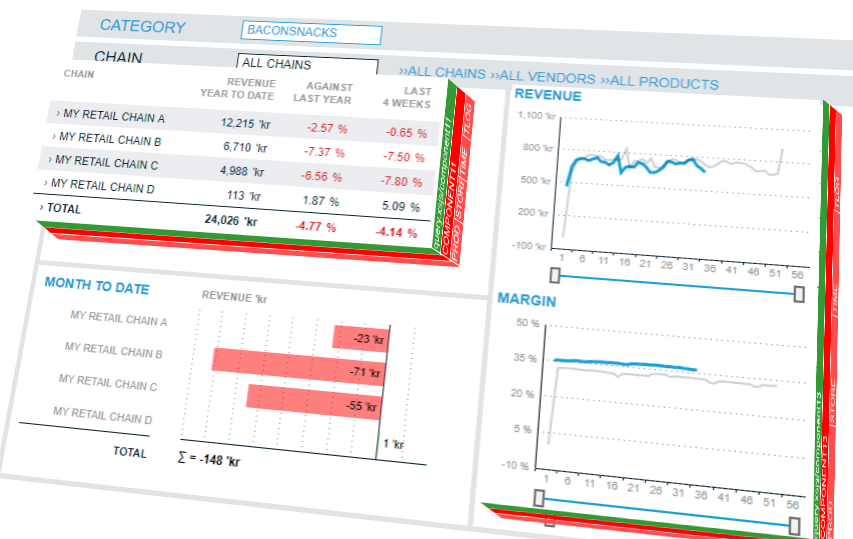
\includegraphics[width=1.00\linewidth]{img/pos3d.png}
	\caption{3D visualization of the software stack in the front-end. Developers can tilt the page to read debugging information on the side of the stacks.}
	\label{fig:3d}
\end{figure}

The interaction diagram was perceived as equally useful.
The developers generally liked the idea of not arranging elements based on timing related information, which allows for a clearer visualization of the logical connections between the application's sub-systems.
Compared to the network log of the browser's development tools that is typically used to get this information, this would be an improvement.
However, they also conceded that sometimes the timing of requests is important, for example when debugging performance bugs or understanding racing conditions caused by concurrent side effects.
Being able to toggle between a time-based and a logical layout would allow developers to get the best of both worlds.

Finally, all developers liked being able to go back and forth in time while following the application flow across layer boundaries.
The possibility to restart an execution without having to craft a corresponding request was already perceived as a huge improvement over existing tools.
Three developers emphasized the usefulness of being able to specify custom request methods with XPath, because they used a custom SQL query builder in their projects.

\subsection{Generalization of Our Results}

Our prototype requires that omniscient debugging is possible on each individual application layer.
However, based on the developer feedback we identified a few "low-hanging fruits" for debugging tools.
For example, developers enjoyed the visualizations of the sub-system interactions.
Collecting the necessary data for such visualizations should be easily possible with today's tools.
Many systems allow to log all requests that are sent or received and the coverage data collected by typical profiling tools is enough to restore the application flow.
Second, restarting an execution from a request can be automated.
Most requests are not large in size and can be stored for the length of a debug session, allowing developers to restart with the push of a button.
Both features combined already allow for a greatly improved debugging workflow, while no detailed tracing for back-in-time debugging is needed.
Tools like Recon or the Path Suite~\cite{lee11:unified_debugging_of_distributed, perscheid13:test-driven_fault_navigation} already use automated restarting to optimize execution tracing.

We developed our debugger to work with a SAPUI5 front-end, an SAP HANA JavaScript application layer, and SAP HANA stored procedures.
To extend our prototype to support more programming languages and technologies, two problems have to be solved.
First, there must be a solution for back-in-time debugging within the respective environment, e.g., by recording detailed traces.
Second, the requests sent and received must be identifiable in such a way that they can be matched with the requests and responses collected from other layers.
Both problems are highly technology-specific. 
However, once a solution is found it can be encapsulated in a module that then extends a meta-debugger such as our prototype.

\section{Conclusion}
\label{sec:conclusion}

With the rising popularity of service-oriented architectures and micro-services in particular, the need for debugging tools that support complex heterogeneous systems is steadily increasing.
We presented a back-in-time debugger that allows the seamless debugging of a 3-tier application stack.
The feature set of our prototype was based on insights gained from interviewing developers who work on modern business applications handling large amounts of data.

Two visualizations help navigating the full execution across all layers, while individual layers can be debugged with back-in-time debugging.
We showed our prototype to developers and received promising feedback regarding the usefulness of the visualizations and their integration with a debugger.

For future work, we wish to enable code analysis across layer boundaries.
If, for example, an object in the application layer is serialized as JSON and then materialized as a JavaScript object in the front-end, an approach is needed to link the fields of both objects in a way that does not require analyzing the JSON serialization and de-serialization logic.

However, as our interviews have shown, even a basic integration of tools can already be a great improvement for developer productivity.
Modular IDEs such as Eclipse allow adding support for new programming languages and technologies via plug-ins with standardized interfaces.
Now, a similar architecture is needed for debuggers to allow not only the development, but also debugging of heterogeneous systems.

\tmpEnd

% events:
% tolmach
% lewis?
% boothe00

\chapter{Related Work}

In this chapter, we present studies and debugging tools related to our contributions.
In \cref{sec:rw_studies}, we examine studies on how developers debug and use debugging tools.
\Cref{sec:rw_bit_debugging} discusses back-in-time debuggers.
\Cref{sec:rw_dynamic_slicing} gives an overview over slicing algorithms.
In \cref{sec:rw_slice_debugging}, we compare debugging tools that use slicing or related techniques to aide developers.
\Cref{sec:rw_system_debugging} and 
\cref{sec:rw_visualization}


\section{Studies}
\label{sec:rw_studies}

Many studies examined how developers approach software maintenance tasks with and without specialized tools.
The requirements we defined for the debugging approaches that form the contribution of this work, as described in \cref{sec:requirements}, "\nameref{sec:requirements}", are based on the outcomes of these studies.
Here, we present a selection of notable studies in our field and their results.

Gould let 10 experienced developers locate bugs in Fortran programs~\cite{gould75:some_psychological_evidence}.
He found that developers can locate bugs up to three times faster when they were familiar with the code.\todo{...}
Furthermore, developers were reluctant to use interactive debugging tools as along as they believed they could find the bug by just reading the code.

Gugerty and Olson studied the difference between novice and expert programmers~\cite{gugerty86:comprehension_differences_in_debugging}.
In the study, both experts and novices used the same strategies to approach fault localization.
However, experts showed superior skills at program comprehension, as they not only required less time needed to form initial hypotheses, but also had initial hypotheses of significantly higher quality.
The quality of program understanding strongly correlated with the quality of fixes.
Novices not only took much longer to develop a fix, they also often introduced additional bugs in the process.

Storey \etal explored the question of how program understanding tools change the way developers approach program comprehension~\cite{storey97:how_do_program_understanding}.
Three software exploration tools that provide visual abstractions were used to solve high-level program understanding tasks.
The study found that programmers approach program comprehension with a variety of strategies and tools were most effective if they supported the developer's preferred strategy instead of imposing a different approach.

In a follow-up study, Storey \etal classified program comprehension strategies and design elements for supporting tools~\cite{storey99:cognitive_design_elements}.
Experienced developers often used a hypothesis-driven top-down approach, but relied on bottom-up strategies to identify abstractions.
In some cases, developers sought to fill only specific gaps in their knowledge of the program, increasing their understanding as needed to locate a bug.
Meta-approaches combine multiple strategies into adaptable tools.
Independently of the strategy, Storey \etal found that program comprehension tools should reduce developers' cognitive overhead by supporting easy navigation and providing orientation in the program.

In two studies, Sillito \etal observed developers working on change tasks to identify their information needs~\cite{sillito06:questions_programmers_ask}.
From this, 44 questions developers frequently ask were derived.
These questions were divided into four categories:
Questions to "find an initial focus point" are most often asked by newcomers, searching for a "place to start looking".
"Building on those points," developers ask questions to understand code in its immediate context.
As the program understanding grows, developers ask questions about sub-graphs, seeking to understand the behavior and purpose of modules.
Finally, developers ask questions over groups of sub-graphs, to understand how different modules interact or relate to each other.
The second and third category contain many questions about program behavior and control flow that can not be easily answered with traditional debugging tools.

While previous studies only look at individual developers, Ko \etal studied the information needs of developers working in collocated teams~\cite{ko07:information_needs_in_collocated}.
By transcribing work sessions minute by minute, they identified 21 information needs.
Developers often collaborated to find answers to their questions, relying on their coworkers knowledge but also causing interruptions.
Ko \etal found that for many questions, better tool support could reduce the time and overhead needed to find an answer.
In other cases, using better tools can enable better collaboration; for instance, post-mortem debuggers allow sharing a debug session on multiple computers.

Weiser found that common approaches to code modularization often do not properly reflect how developers understand a program~\cite{weiser82:programmers_use_slices_when}.
While code is often grouped in terms of functional relation, developers often prefer to understand code in sets of statements related by control flow, not matching the file or module structure.
In the absence of aspect-oriented modularization, slicing techniques can identify such related sets of statements and thereby support program comprehension.

Johnson \etal interviewed developers to study the usage of software analysis tools~\cite{johnson13:why_dont_software_developers}.
While the study focused on static tools, many of the insights can be transferred to dynamic analysis tools as well.
In the study, all developers reported the examined analysis tools to be useful, but were mostly reluctant to use them on a regular basis, due to multiple barriers.
First, false positives and difficult-to-understand results imposed a high cognitive overhead on developers.
Furthermore, a lack of integration into the regular development workflow (and into the IDE in particular) combined with slow responsiveness caused tools to be more of an interruption than actual help.
This was exacerbated by a lack of customizability to the developers' needs.
Finally, tools that did not support collaboration with coworkers were not adopted by the team as a whole, reducing the usefulness for each individual.

Perscheid \etal studied the adoption of advanced debugging techniques by observing professional software developers and conducting an online survey~\cite{perscheid17:studying_the_advancement}.
They found that while most developers are proficient using a symbolic debuggers, knowledge of more sophisticated debugging techniques is sparse.
Furthermore, developers in the study reported a long distance between observed failure and root cause as the main difficulty of finding bugs and wished for more easily accessible debugging tools.

\section{Back-in-Time Debugging}
\label{sec:rw_bit_debugging}

%A symbolic debugger allows developers to inspect the program state at single points in time only.
%Having access to a program's execution history can be beneficial to developers in multiple ways, for example to run analyses on the execution or to follow an infection chain backwards through time.

Reversing a program execution was for the first time made possible with the EXDAMS debugging system~\cite{balzer69:exdams_extendable_debugging}.
Since then, many debuggers that use execution history or back-in-time operations have been developed and various approaches with different advantages and draw-backs were tested.

Powell and Linton developed a debugging environment that stores a program's code, state, and execution history in a relational database~\cite{powell83:a_database_model}.
Using this system, developers can express questions about program behavior as database queries.
This allows developers to formulate complex questions with high precision.

IGOR is a snapshot-based back-in-time debugger by Feldman and Brown~\cite{feldman88:igor_a_system}.
By delegating the creation and management of snapshots to the operating system, the performance overhead is kept low.
IGOR supports reversing execution, searching the execution history, and substituting data and program parts during execution.

Tolmach and Appel developed a snapshot-based back-in-time debugger that operates at the source level~\cite{tolmach93:a_debugger_for_standard}.
The program code is pre-processed before compilation to facilitate back-in-time debugging without the need for changes to the compiler or runtime environment.
Creating snapshots as first-class continuations reduces the complexity of the debugging system by reusing respective interpreter functionality to replace execution.
%creates checkpoints as first-class continuations. This
%allows a flexible mechanism to replace execution and to provide reverse execution for
%the user and the interpreter.

ZStep95 is a back-in-time debugger for LISP by Lieberman and Fry that keeps a full execution history to reverse control flow~\cite{lieberman95:zstep_95_a_reversible}.
This way, individual instructions can be reversed faster than with a snapshot-based approach.
Furthermore, ZStep95 records the screen to include the user interface in the debug session.
Developers can jump to the previous or next UI change, debugging a program by its observable behavior.

Boothe developed a snapshot-based back-in-time debugger for C and C++~\cite{boothe00:efficient_algorithms_for_bidirectional}.
I/O logging ensures the deterministic re-execution between checkpoints and a sequential numbering of events allows the debugger to identify events across multiple re-executions.
Memory overhead is reduced through exponential checkpoint thinning, based on the idea that developers are more likely to reverse execution in small steps and that longer waiting times for larger steps are acceptable.

Cook developed a semantic model for the reverse execution of stack-based bytecode languages~\cite{cook02:reverse_execution_of_java}.
A prototype debugger using this model was implemented in a Java VM.
The model retains information otherwise lost during state-changing operations.
This allows the debugger to execute the program backwards, but not to jump to previous points in time or to search the execution history.

In 2003, Lewis presented the Omniscient Debugger for Java~\cite{lewis03:debugging_backwards_in_time}.
With an omniscient debugger, the entire execution history is searchable and state from any point-in-time can be restored in constant time.
The latter is achieved using a post-mortem approach.
Instead of rewinding the actual program, the debugger only presents the program state, as it was, in its user interface.

UNSTUCK is an omniscient debugger for Smalltalk by Hofer \etal~\cite{hofer06:design_and_implementation}.
It is directly integrated in the IDE and features searching and code highlighting.

To better support the large execution traces required by omniscient debuggers, Pothier \etal developed a distributed database to store and search traces~\cite{pothier07:scalable_omniscient_debugging}.
While this system is very efficient, it has high requirements in terms of physical resources and set-up.
Later, Pothier and Tanter developed an approach for summarizing and indexing traces that supports querying arbitrarily large traces efficiently~\cite{pothier11:summarized_trace_indexing}.
Partial re-execution of program parts is used to retrieve information that was discarded to save memory.
A similar approach was used by Perscheid to achieve efficient back-in-time debugging with the Path tool suite~\cite{perscheid13:test-driven_fault_navigation}.

Lienhard \etal developed a system for back-in-time debugging that reduces memory overhead by using the underlying VM's garbage collector~\cite{lienhard08:practical_object-oriented_back-in-time_debugging}.
They extended the Squeak Smalltalk VM to store object history along with the regular object.
When an object is no longer reachable, its history is considered irrelevant and will be discarded, too.

TARDIS by Barr and Marron is a back-in-time debugger for the .net runtime~\cite{barr14:tardis_affordable_time-travel_debugging}.
TARDIS uses a combination of snapshots and logging and is integrated in the runtime environment, thereby achieving very low run-time and memory overhead.
A similar debugger was developed for Microsoft’s open-source ChakraCore JavaScript engine and the Node.js application framework~\cite{barr16:time-travel_debugging_for_javascriptnode}.
The debugger supports both live debugging with snapshots and post-mortem debugging from logs.

RR is a debugger that can record and replay arbitrary programs in Linux without modifications to the program code, the compilation pipeline, the runtime environment, or the operating system~\cite{ocallahan17:engineering_record_and_replay}.
This allows RR to be used as a general purpose debugger with low set-up and maintenance costs.

\section{Dynamic Slicing Algorithms}
\label{sec:rw_dynamic_slicing}

A history of different slicing approaches was already presented in \cref{sec:evolution_of_slicing}, "\nameref{sec:evolution_of_slicing}".
In this section, we present


\cite{ottenstein84:the_program_dependence_graph}
represent program as pdg, faster through reuse. better results.

\cite{korel88:dynamic_program_slicing}
executable dynamic slicing.

\cite{agrawal90:dynamic_program_slicing}
Dynamic slicing. Dynamic dependence graph. n algorithms


\cite{venkatesh95:experimental_results_from_dynamic}
C slicer, different algorithms for data, control, executable slices.

\cite{venkatesh91:the_semantic_approach}!!!

\cite{hall95:automatic_extraction_of_executable}
dynamic, executable slice for multiple inputs

\cite{hoffner95:evaluation_and_comparison}
survey of slicing tools

\cite{korel98:dynamic_program_slicing_methods}
overview of slicing algorithms

\cite{wang08:dynamic_slicing_on_java}
JSlice for java bytecode traces

\cite{wong16:a_survey_on_software}
recent survey of automated fault localization


\section{Slicing-based Debugging}
\label{sec:rw_slice_debugging}
x
\newpage

\cite{agrawal93:debugging_with_dynamic_slicing}
SPYDER
dynamic slicing with execution backtracking with checkpoints
user can also choose only data or control

\cite{ko08:debugging_reinvented_asking}
why and why not questions. dynamic and static

\cite{perscheid13:test-driven_fault_navigation}
The Path tool suite and its Test-Driven Fault Navigation~\cite{perscheid2013} leverages reproducible test cases in order to distribute the tracing overhead over multiple runs depending on developers' needs.



\cite{sakurai15:the_omission_finder}
Using Traceglasses \cite{sakurai10:traceglasses_a_trace-based_debugger} trace-based bit for java,
pointer assignment graphs and control flow graphs to locate omission bugs

\section{System Debuggers}
\label{sec:rw_system_debugging}
x
\newpage


The idea of being able to debug backwards in time dates back to the 1960s with EXDAMS, a debugger for FORTRAN \cite{balzer_exdams_1969}.
Since then, debuggers with back-in-time capabilities have been implemented for many programming languages \cite{agrawal_debugging_1993, feldman_igor_1988, lieberman_zstep_1997}.

In 2003, Lewis introduced the concept of "omniscient debugging", a debugger that can not only rewind time, but has instant access to every point in past and future~\cite{lewis_debugging_2003}.
Later work on omniscient debugging focused mostly on handling the large amounts of data such a debugger creates~\cite{pothier_scalable_2007, lienhard_practical_2008}.
Perscheid et al. \cite{perscheid_testdriven_2013} combined omniscient debugging and spectrum-based fault analysis, analyzing a suite of unit tests with passing and failing test cases.
%Perscheid et al. \cite{perscheid_test-driven_2013} combined omniscient debugging and dynamic code analysis similar to slicing to automatically identify likely locations for code defects by analyzing a suite of unit tests with passing and failing test cases.

Lanza showed the importance of visualizations in software development~\cite{lanza2003program}.
SHriMP views are one example how such visualizations can guide developers~\cite{storey2002shrimp}.
Baecker et al. used visualizations to improve the debugging process by animating algorithms~\cite{baecker1997software}.
Moher~\cite{moher1988provide} and Beguelin et al.~\cite{beguelin1993visualization} used visualizations to support the understanding of process interactions in heterogeneous environments.
However, in both works the focus was set more on understanding and debugging applications on an architectural level, while we aim to integrate debugging of individual components as if the software was a single program.

%SPYDER is a debugger with slicing and back-and-time capabilites \cite{agrawal_debugging_1993}.
%With SPYDER, Agrawal et al. also proposed a new debugging workflow that is similar to our approach.
%However, while Agrawal et al. proposed to create a new slice every time the programmers question changed, our approach focuses on iteratively modifying a single slice.
%Furthermore, we present a new way of presenting aspects of the slice to developers.
Our approach requires that searchable traces are available for all sub-systems of an application.
Solutions for collecting and storing execution traces always depend on the underlying technology, nevertheless some general approaches exist.
Mellor-Crummey and LeBlanc showed how to obtain instruction pointers in software when they are not provided by the system, which is a general requirement for tracing~\cite{mellor-crummey_software_1989}.
With PQL, developers can search for the occurrence of code examples in program executions~\cite{martin_finding_2005}.
Similarly, Recon is a debugging tool that allows to query the execution of distributed systems with SQL-like queries~\cite{lee_unified_2011}.
Recon's query interface can not only provide all the information a debugger would need.
O'Callahan et al. presented a generic approach for recording and replaying program executions~\cite{ocallahan_engineering_2017}.


\section{Visualizations for Program Comprehension}
\label{sec:rw_visualization}

\cite{olsson91:sequential_debugging_at}
Dalek, debugger with hierarchy events, events extracted from sequential code.


\chapter{Conclusion}
\section{Towards Full-System Debuggers}


\section{Future Work}

\newpage
x
\newpage
x
\newpage
x
\newpage
x


%\defaultstatement

%\printglossaries

\emergencystretch=3em
\printbibliography[heading=bibintoc,category=cited]

\printbibliography[title={TODO},notcategory=cited]

\end{document}
